%%%%%%%%%%%%%%%%%%%%%%%%%%%%%%%%%%%%%%%%%%%%%%%%%%%%%%%%%%%%%%%%%%%%%
%
% Complete documentation on the extended LaTeX markup used for Insight
% documentation is available in ``Documenting Insight'', that is part
% of the standard documentation for Insight.  It may be found online
% at:
%
%                    http://www.itk.org
%
%%%%%%%%%%%%%%%%%%%%%%%%%%%%%%%%%%%%%%%%%%%%%%%%%%%%%%%%%%%%%%%%%%%%%

\documentclass{InsightSoftwareGuide}


\usepackage[dvips]{graphicx}
\usepackage{times,lscape,url}
%\usepackage{mdwtab}


%%% \usepackage[latin1]{inputenc}
%%% \selectlanguage{french}
% Configuration pour les accents francais pour l'OTB
\usepackage[latin1]{inputenc}
%\usepackage[french]{babel}
\usepackage{tikz}

\usepackage{color}

\definecolor{listcomment}{rgb}{0.0,0.5,0.0}
\definecolor{listkeyword}{rgb}{0.0,0.0,0.5}
\definecolor{listnumbers}{gray}{0.65}
\definecolor{listlightgray}{gray}{0.955}
\definecolor{listwhite}{gray}{1.0}

\usepackage{minted}
\newminted{cpp}{fontsize=\small}
\newminted{cmake}{fontsize=\small}
\newminted{bat}{fontsize=\small}

\usepackage{mdframed}
\BeforeBeginEnvironment{cppcode}{\begin{mdframed}[leftline=false,rightline=false,backgroundcolor=listlightgray]}
\AfterEndEnvironment{cppcode}{\end{mdframed}}

\newif\ifitkFullVersion
\itkFullVersiontrue
%\itkFullVersionfalse

\newif\ifitkPrintedVersion
\itkPrintedVersiontrue
%\itkPrintedVersionfalse

\usepackage{multicol}

%%%%%%%%%%%%%%%%%%%%%%%%%%%%%%%%%%%%%%%%%%%%%%%%%%%%%%%%%%%%%%%%%%
%
%  hyperref should be the last package to be loaded.
%
%%%%%%%%%%%%%%%%%%%%%%%%%%%%%%%%%%%%%%%%%%%%%%%%%%%%%%%%%%%%%%%%%%
\ifitkPrintedVersion
\usepackage[dvips,
pdftitle={OTB Software Guide},
pdfauthor={CNES},
pdfsubject={Remote Sensing, Orfeo, Pleiades, Cosmo Skymed},
pdfkeywords={Image processing, Remote sensing, Guide},
pdfpagemode={UseOutlines},
bookmarks,bookmarksopen,
pdfstartview={FitH},
backref,
colorlinks,linkcolor={black},citecolor={black},urlcolor={black},
]{hyperref}
\else
\usepackage[dvips,
pdftitle={OTB Software Guide},
pdfauthor={CNES},
pdfsubject={Remote Sensing, Orfeo, Pleiades, Cosmo Skymed},
pdfkeywords={Image processing, Remote sensing, Guide},
pdfpagemode={UseOutlines},
bookmarks,bookmarksopen,
pdfstartview={FitH},
backref,
colorlinks,linkcolor={blue},citecolor={blue},urlcolor={blue},
]{hyperref}
\fi

\usepackage{amsmath,amssymb,amsfonts}
\usepackage{bbm}
%%%%%%%%%%%%%%%%%%%%%%%%%%%%%%%%%%%%%%%%%%%%%%%%%%%%%%%%%%%%%%%%%%%
%
%
%   Load configuration parameters prepared by CMake
%
%
%%%%%%%%%%%%%%%%%%%%%%%%%%%%%%%%%%%%%%%%%%%%%%%%%%%%%%%%%%%%%%%%%%%

\input{SoftwareGuideConfiguration.tex}

\def\logoCNES{CNES_nom.eps}

\newtheorem{algo}{Algorithm}
\newtheorem{defin}{Definition}
%%%%%%%%%%%%%%%%%%%%%%%%%%%%%%%%%%%%%%%%%%%%%%%%%%%%%%%%%%%%%%%%%%%
%
%
%           The Insight Toolkit Software Guide
%
%
%%%%%%%%%%%%%%%%%%%%%%%%%%%%%%%%%%%%%%%%%%%%%%%%%%%%%%%%%%%%%%%%%%%

\title{The ORFEO Tool Box Software Guide\\ Updated
  for OTB-\otbversion}

\author{OTB Development Team}

\authoraddress{
  \url{http://www.orfeo-toolbox.org}\\
  e-mail: \email{otb@cnes.fr}
}

\date{\today}


% actually write the .idx file
\makeindex

\setcounter{tocdepth}{3}



%%%%%%%%%%%%%%%%%%%%%%%%%%%%%%%%%%%%%%%%%%%%%%%%%%%%%%%%%%%%%%%%%%%
%
%           Begin Document
%
%%%%%%%%%%%%%%%%%%%%%%%%%%%%%%%%%%%%%%%%%%%%%%%%%%%%%%%%%%%%%%%%%%%

\begin{document}

\ifitkPrintedVersion
%% \input{PrintedPreamble.tex}
\fi

\maketitle

\frontmatter

\hyperbaseurl{http://www.orfeo-toolbox.org}


%%%%%%%%%%%%%%%%%%%%%%%%%%%%%%%%%%%%%%%%%%
%
%  Page with OTB logo
%
%%%%%%%%%%%%%%%%%%%%%%%%%%%%%%%%%%%%%%%%%%
\cleardoublepage

\begin{minipage}[t][10cm][b]{\textwidth}
\center
\includegraphics[width=0.5\textwidth]{logoVectoriel.eps}
\large
\begin{center}
\emph{The ORFEO Toolbox is not a black box.}\\
\end{center}
\hspace{8cm} Ch.D.
\normalsize
\end{minipage}



%%%%%%%%%%%%%%%%%%%%%%%%%%%%%%%%%%%%%%%%%%%%%%
%
% remove headings from the following material
\pagestyle{plain}
%
%%%%%%%%%%%%%%%%%%%%%%%%%%%%%%%%%%%%%%%%%%%%%%



%%\ifitkPrintedVersion
%% \input{Cover.tex}
%%\fi

\input{Abstract.tex}




%%%%%%%%%%%%%%%%%%%%%%%%%%%%%%%%%%%%%%%%%%%%%%%%%%%%%%%%%
%
% Insert Table of Contents; List of Figures and Tables
%
%%%%%%%%%%%%%%%%%%%%%%%%%%%%%%%%%%%%%%%%%%%%%%%%%%%%%%%%%


%%%%%%%%%%%%%%%%%%%%%%%%%%%%%%%%%%%%%%%%%%%%%%
%
% enable headings from the following material
\pagestyle{normal}
%
%%%%%%%%%%%%%%%%%%%%%%%%%%%%%%%%%%%%%%%%%%%%%%
\small
\tableofcontents
\listoffigures
\listoftables
\normalsize




%%%%%%%%%%%%%%%%%%%%%%%%%%%%%%%%%%%%%%%%%
%
% Begin technical content
%
%%%%%%%%%%%%%%%%%%%%%%%%%%%%%%%%%%%%%%%%%

\mainmatter

\part{Introduction}\label{part:introduction}

\chapter{Welcome}
\label{chapter:Welcome}

Welcome to the \emph{ORFEO ToolBox (OTB) Software Guide}.

This document presents the essential concepts used in OTB. It will
guide you through the road of learning and using OTB. The Doxygen
documentation for the OTB application programming interface is
available on line at \url{https://www.orfeo-toolbox.org/doxygen}.

\section{Organization}
\label{sec:Organization}

This software guide is divided into several parts, each of which is further
divided into several chapters. Part~\ref{part:introduction} is a general
introduction to OTB,
with---in the next chapter---a description of how to install the ORFEO
Toolbox on your computer. Part~\ref{part:introduction} also
introduces basic system concepts such as an overview of the system
architecture, and how to build applications in the C++ programming
language. Part \ref{part:tutorials} is a short guide with gradual difficulty to
get you start programming with OTB. Part~\ref{part:userguide} describes the
system from the user point of view. Dozens
of examples are used to illustrate important system features.
Part~\ref{part:developerguide}  is for
the OTB developer. It explains how to create your own classes and extend
the system.%, and interface to windowing and GUI systems.

\section{How to Learn OTB}
\label{sec:HowToLearnOTB}

There are two broad categories of users of OTB. First are class
developers, those who create classes in C++. The second, users, employ
existing C++ classes to build applications. Class developers must be
proficient in C++, and if they are extending or modifying OTB, they
must also be familiar with OTB's internal structures and design
(material covered in Part~\ref{part:developerguide}).

The key to learning how to use OTB is to become familiar with its
palette of objects and the ways of combining them. We recommend that you learn
the system by studying the
examples and then, if you are a class developer, study the source
code. Start by the first few tutorials in Part~\ref{part:tutorials} to get
familiar with the build process and the general program organization, follow by
reading Chapter \ref{chapter:SystemOverview}, which provides an overview of some
of the key concepts in the system, and then review the examples in
Part~\ref{part:userguide}. You may also wish to compile and run the dozens of
examples
distributed with the source code found in the directory
\code{OTB/Examples}. (Please see the file
\code{OTB/Examples/README.txt} for a description of the examples
contained in the various subdirectories.) There are also several
hundreds of tests found in the source distribution in
\code{OTB/Testing/Code}, most of which are minimally documented
testing code. However, they may be useful to see how classes are used
together in OTB, especially since they are designed to exercise as
much of the functionality of each class as possible.

\section{Software Organization}
\label{sec:SoftwareOrganization}

The following sections describe the directory contents, summarize the
software functionality in each directory, and locate the documentation and
data.

\subsection{Obtaining the Software}
\label{sec:ObtainingTheSoftware}

Periodic releases of the software are available on the OTB Website. These
official releases are available a few times a year and announced on the ORFEO
Web pages and mailing lists.

This software guide assumes that you are working with the latest official OTB
release (available on the OTB Web site). %If you are a new user,
%we highly recommend that you use the released version of the software.


OTB can be downloaded without cost from the following web site:
\begin{center}
  \url{http://www.orfeo-toolbox.org/}
\end{center}
In order to track the kind of applications for which OTB is being used, you
will be asked to complete a form prior to downloading the software.
The information you provide in this form will help developers to get a better
idea of the interests and skills of the toolkit users.

Once you fill out this form you will have access to the download
page. This page can be book marked to facilitate subsequent visits to
the download site without having to complete any form again.

 Then choose the tarball that better fits your system. The options
are \code{.zip} and \code{.tgz} files.  The first type is better suited for
MS-Windows while the second one is the preferred format for UNIX systems.

Once you unzip or untar the file, a directory called \code{OTB} will be
created in your disk and you will be ready for starting the configuration
process described in the CookBook.


There are two other ways of getting the OTB source code:
\begin{itemize}
\item Clone the current release with \href{https://git-scm.com/}{Git} from the
  \href{https://gitlab.orfeo-toolbox.org/orfeotoolbox/otb.git}{OTB git server}, (master branch)
\item Clone the latest revision with \href{https://git-scm.com/}{Git} from the
  \href{https://gitlab.orfeo-toolbox.org/orfeotoolbox/otb.git}{OTB git server} (develop branch).
\end{itemize}

These last two options need a proper \href{https://git-scm.com/}{Git} installation. To get source code from Git, do:
\begin{verbatim}
git clone https://gitlab.orfeo-toolbox.org/orfeotoolbox/otb.git
\end{verbatim}

Using Git, you can easily navigate through the different versions. The master
branch contains the latest stable version:
\begin{verbatim}
git checkout master
\end{verbatim}
Specific versions are availables with tags:
\begin{verbatim}
git checkout 5.2.0
\end{verbatim}
Finally, this brings you to the latest development version:
\begin{verbatim}
git checkout develop
\end{verbatim}

There is also a mirror of OTB official repository on \href{https://github.com/orfeotoolbox/OTB}{GitHub}.
You can find more information on the OTB git workflow in the \href{http://wiki.orfeo-toolbox.org/index.php/Git}{wiki}.

\subsection{Directory Structure}
\label{sec:DirectoryStructure}

To begin your OTB odyssey, you will first need to know something about OTB's
software organization and directory structure. It is helpful to know enough to
navigate through the code base to find examples, code, and documentation.

The \code{OTB} contains the following subdirectories:
\begin{itemize}
        \item \code{OTB/Modules}---the heart of the software; the location
        of the majority of the source code.
        \item \code{OTB/CMake}---internal files used during the
        configuration process.
        \item \code{OTB/Copyright}---the copyright information of OTB
        and all the dependencies included in the OTB source tree.
        \item \code{OTB/Examples}---a suite of simple, well-documented
        examples used by this guide and to illustrate important
        OTB concepts.
        \item \code{OTB/Superbuild}---CMake scripts to automatically download, patch, build and install important
        dependencies of OTB (ITK, OSSIM, GDAL to name a few).
        \item \code{OTB/Utilities}---small programs used for the maintenance of OTB.
\end{itemize}


OTB is organized into different modules, each one covering different part of image processing.
It is therefore important to understand the source code directory structure---found in \code{OTB/Modules}---.
\begin{itemize}
  \item \code{OTB/Modules/Adapters}---Adapters for Boost, Curl, Gdal and Ossim.
  \item \code{OTB/Modules/Applications}---a set of applications modules that can be launched in different ways
    (command-line, graphical interface, Python/Java), refer to the OTB Cookbook for more information.
  \item \code{OTB/Modules/Core}---core classes, macro definitions,
  typedefs, and other software constructs central to OTB.
  \item \code{OTB/Modules/Detection}---detection of clouds, roads.
  \item \code{OTB/Modules/Feature}---various local descriptors and features.
  \item \code{OTB/Modules/Filtering}---basic image processing filters.
  \item \code{OTB/Modules/Fusion}---image fusion algorithms, as for
  instance, pansharpening.
  \item \code{OTB/Modules/Hyperspectral}---hyperspectral images analysis.
  \item \code{OTB/Modules/IO}---classes that support the reading
  and writing of data.
  \item \code{OTB/Modules/Learning}---several functionalities for
	supervised learning and classification.
  \item \code{OTB/Modules/OBIA}---Object Based Image Analysis filters
	and data structures.
  \item \code{OTB/Modules/Radiometry}---classes allowing to compute
  vegetation indices and radiometric corrections.
  \item \code{OTB/Modules/Registration}---classes for registration of images or other data structures to each other.
  \item \code{OTB/Modules/Remote}---Functions to fetch remote modules.
  \item \code{OTB/Modules/Segmentation}---several functionalities for image segmentation.
  \item \code{OTB/Modules/ThirdParty}---Modules that import OTB's dependencies.
  \item \code{OTB/Modules/Wrappers}---Applications wrappers with several access points (command-line, QT Gui, SWIG\ldots).
\end{itemize}


See also chapter \ref{chapter:newModules} for more information about how to write modules.

\subsection{Documentation}
\label{sec:Documentation}

Besides this text, there are other documentation resources that you should be
aware of.
\begin{description}
        \item[Doxygen Documentation.] The Doxygen documentation is an
        essential resource when working with OTB. These extensive Web
        pages describe in detail every class and method in the
        system. The documentation also contains inheritance and
        collaboration diagrams, listing of event invocations, and data
        members. The documentation is heavily hyper-linked to other
        classes and to the source code. The Doxygen documentation is
        available on-line at
        \url{http://www.orfeo-toolbox.org/doxygen/}.

	\item[Header Files.] Each OTB class is implemented with a .h and
        .cxx/.hxx file (.hxx file for templated classes). All methods
        found in the .h header files are documented and provide a quick way
        to find documentation for a particular method. (Indeed, Doxygen uses
        the header documentation to produces its output.)
\end{description}

\subsection{Data}
\label{sec:Data}

The OTB Toolkit was designed to support the ORFEO Acompaniment Program
and its associated data. This data is available at
\url{http://smsc.cnes.fr/PLEIADES/index.htm}.



\section{The OTB Community and Support}
\label{sec:AdditionalResources}

\subsection{Join the Mailing List}
\label{sec:JoinMailList}

\index{OTB!mailing list}
\index{mailing list}

It is strongly recommended that you join the users mailing list. This is one
of the primary resources for guidance and help regarding the use of the
toolkit. You can subscribe to the users list online at

\begin{center}
\url{http://groups.google.com/group/otb-users}
\end{center}

The otb-users mailing list is also the best mechanism for expressing your
opinions about the toolbox and to let developers know about features that you
find useful, desirable or even unnecessary. OTB developers are committed to
creating a self-sustaining open-source OTB community. Feedback from users is
fundamental to achieving this goal.

\subsection{Community}
OTB was created from its inception as a collaborative, community
effort. Research, teaching, and commercial uses of the toolkit are
expected. If you would like to participate in the community, there are a
number of possibilities.

\begin{itemize}
       \item Users may actively report bugs, defects in the system API,
       and/or submit feature requests. Currently the best way to do this is
       through the OTB users mailing list.

       \item Developers may contribute classes or improve existing
       classes. If you are a developer, you may request permission to join
       the OTB developers mailing list. Please do so by sending email to
       otb ``at'' cnes.fr. To become a developer you need to
       demonstrate both a level of competence as well as
       trustworthiness. You may wish to begin by submitting fixes to the OTB
       users mailing list.

       \item Research partnerships with members of the ORFEO
       Acompaniment Program are encouraged. CNES will encourage the use of
       OTB in proposed work and research projects.

%%        \item For those developing commercial applications with OTB,
%%        support and consulting are available from Kitware at
%%        \url{http://www.kitware.com}. Kitware also offers short OTB courses
%%        either at a site of your choice or periodically at Kitware.

       \item Educators may wish to use OTB in courses. Materials are being
       developed for this purpose, e.g., a one-day, conference course and
       semester-long graduate courses. Watch the OTB web pages or check in
       the \code{OTB-Documents/CourseWare} directory for more information.
\end{itemize}

Orfeo ToolBox is currently in the incubation stage of being part of the
OSGeo\footnote{http://www.osgeo.org/} foundation.Within the ORFEO ToolBox
community we act respectfully toward others in line with the OSGeo Code of
Conduct\footnote{http://www.osgeo.org/code\_of\_conduct}.


\section{A Brief History of OTB}
\label{sec:History}

\index{OTB!history}


Beside the Pleiades (PHR) and Cosmo-Skymed (CSK) systems developments forming
ORFEO, the dual and bilateral system (France - Italy) for Earth Observation, the
ORFEO Accompaniment Program was set up, to prepare, accompany and promote the
use and the exploitation of the images derived from these sensors.

The creation of a preparatory
program\footnote{http://smsc.cnes.fr/PLEIADES/A\_prog\_accomp.htm} is needed
because of :
\begin{itemize}
\item the new capabilities and performances of the ORFEO systems (optical and
radar high resolution, access capability, data quality, possibility to acquire
simultaneously in optic and radar),
\item the implied need of new methodological developments : new processing
methods, or adaptation of existing methods,
\item the need to realize those new developments in very close
  cooperation with the final users for better integration of new products in
their systems.

\end{itemize}

This program was initiated by CNES mid-2003 and will last until 2010 at least
It consists in two parts, between which it is necessary to keep a strong
interaction :
\begin{itemize}
\item A Thematic part
\item A Methodological part.
\end{itemize}

The Thematic part covers a large range of applications (civil and
defence ones), and aims at specifying and validating value added
products and services required by end users. This part includes
consideration about products integration in the operational systems or
processing lines. It also includes a careful thought on intermediary
structures to be developed to help non-autonomous users. Lastly, this part aims
at raising future users awareness, through practical demonstrations and
validations.

The Methodological part objective is the definition and the
development of tools for the operational exploitation of the future
submetric optic and radar images (tridimensional aspects, change
detection, texture analysis, pattern matching, optic radar
complementarities). It is mainly based on R\&D studies and doctorate
and post-doctorate research.

In this context, CNES\footnote{http://www.cnes.fr} decided to develop
the \emph{ORFEO ToolBox} (OTB), a set of algorithms encapsulated in a
software library. The goals of the OTB is to capitalize a methological
\textit{savoir faire} in order to adopt an incremental development
approach aiming to efficiently exploit the results obtained in the
frame of methodological R\&D studies.

All the developments are based on FLOSS (Free/Libre Open Source
Software) or existing CNES developments.

OTB is implemented in C++ and is mainly based on
ITK\footnote{http://www.itk.org} (Insight Toolkit):
\begin{itemize}
  \item ITK is used as the core element of OTB
  \item OTB classes inherit from ITK classes
  \item The software development procedure of OTB is strongly inspired
  from ITK's (Extreme Programming, test-based coding, Generic
  Programming, etc.)
  \item The documentation production procedure is the same as for ITK
  \item Several chapters of the Software Guide are literally copied
  from ITK's Software Guide (with permission).
  \item Many examples are taken from ITK.
\end{itemize}

\subsection{ITK's history}

In 1999 the US National Library of Medicine of the National Institutes of
Health awarded six three-year contracts to develop an open-source
registration and segmentation toolkit, that eventually came to be known as
the Insight Toolkit (ITK) and formed the basis of the Insight Software
Consortium. ITK's NIH/NLM Project Manager was Dr. Terry Yoo, who coordinated the
six prime contractors composing the Insight consortium. These consortium
members included three commercial partners---GE Corporate R\&D, Kitware,
Inc., and MathSoft (the company name is now Insightful)---and three academic
partners---University of North Carolina (UNC), University of Tennessee (UT)
(Ross Whitaker subsequently moved to University of Utah), and University of
Pennsylvania (UPenn). The Principle Investigators for these partners were,
respectively, Bill Lorensen at GE CRD, Will Schroeder at Kitware, Vikram
Chalana at Insightful, Stephen Aylward with Luis Ib\'a\~nez at UNC (Luis is now
at Kitware), Ross Whitaker with Josh Cates at UT (both now at Utah), and
Dimitri Metaxas at UPenn (now at Rutgers). In addition, several
subcontractors rounded out the consortium including Peter Raitu at Brigham \&
Women's Hospital, Celina Imielinska and Pat Molholt at Columbia University,
Jim Gee at UPenn's Grasp Lab, and George Stetten at the University of
Pittsburgh.

In 2002 the first official public release of ITK was made
available.





\chapter{System Overview}
\label{chapter:SystemOverview}

The purpose of this chapter is to provide you with an overview of the
\emph{ORFEO Toolbox} system. We recommend that you read this chapter to
gain an appreciation for the breadth and area of application of
OTB. In this chapter, we will make reference either to \emph{OTB
  features} or \emph{ITK features} without distinction. Bear in mind
that OTB uses ITK as its core element, so all the fundamental elements
of OTB come from ITK. OTB extends the functionalities of ITK for the
remote sensing image processing community. We benefit from the Open
Source development approach chosen for ITK, which allows us to provide
an impressive set of functionalities with much less effort than
would have been the case in a closed source universe!

\section{System Organization}
\label{sec:SystemOrganization}

The Orfeo Toolbox consists of several subsystems:

\begin{description}
	\item[Essential System Concepts.] Like any software system, OTB is
        built around some core design concepts. OTB uses those of
        ITK. Some of the more important
        concepts include generic programming, smart pointers for memory
        management, object factories for adaptable object instantiation,
        event management using the command/observer design paradigm, and
        multithreading support.

	\item[Numerics] OTB, as ITK uses VXL's VNL numerics libraries. These are
        easy-to-use C++ wrappers around the Netlib Fortran numerical 
        analysis routines (\url{http://www.netlib.org}).

	\item[Data Representation and Access.]  Two principal classes
        are used to represent data: the \doxygen{otb}{Image} and
        \doxygen{itk}{Mesh} classes.  In addition, various types of
        iterators and containers are used in ITK to hold and traverse
        the data. Other important but less popular classes are also
        used to represent data such as histograms.

	\item[ITK's Data Processing Pipeline.]  The data representation
	classes (known as \emph{data objects}) are operated on by
	\emph{filters} that in turn may be organized into data flow
	\emph{pipelines}. These pipelines maintain state and therefore
	execute only when necessary.  They also support
	multi-threading, and are streaming capable (i.e., can operate
	on pieces of data to minimize the memory footprint).

        \item[IO Framework.] Associated with the data processing
        pipeline are \emph{sources}, filters that initiate the
        pipeline, and \emph{mappers}, filters that terminate the
        pipeline.  The standard examples of sources and mappers are
        \emph{readers} and \emph{writers} respectively.  Readers
        input data (typically from a file), and writers output data
        from the pipeline. \emph{Viewers} are another example of mappers.

	\item[Spatial Objects.] Geometric shapes are represented in
        OTB using the ITK spatial object hierarchy.  These classes are
        intended to support modeling of anatomical structures in
        ITK. OTB uses them in order to model cartographic elements. Using a
        common basic interface, the spatial objects are capable of
        representing regions of space in a variety of different
        ways. For example: mesh structures, image masks, and implicit
        equations may be used as the underlying representation scheme.
        Spatial objects are a natural data structure for communicating
        the results of segmentation methods and for introducing
        geometrical priors in both segmentation and registration
        methods.

	\item[ITK's Registration Framework.] A flexible framework for
        registration supports four different types of registration:
        image registration, multiresolution registration, PDE-based
        registration, and FEM (finite element method) registration.

	\item[FEM Framework.] ITK includes a subsystem for solving general
        FEM problems, in particular non-rigid registration. The FEM package
        includes mesh definition (nodes and elements), loads, and boundary
        conditions.

	\item[Level Set Framework.] The level set framework is a set of
        classes for creating filters to solve partial differential equations
        on images using an iterative, finite difference update scheme. The
        level set framework consists of finite difference solvers including a
        sparse level set solver, a generic level set segmentation filter, and
        several specific subclasses including threshold, Canny, and Laplacian
        based methods.

	\item[Wrapping.] ITK uses a unique, powerful system for
	producing interfaces (i.e., ``wrappers'') to interpreted
	languages such as Tcl and Python. The GCC\_XML tool is used to
	produce an XML description of arbitrarily complex C++ code;
	CSWIG is then used to transform the XML description into
	wrappers using the \href{http://www.swig.org/}{SWIG}
	package. OTB does not use this system at present.

%% 	\item[Auxiliary / Utilities] Several auxiliary subsystems are 
%%         available to supplement other classes in the system. For example,
%%         calculators are classes that perform specialized operations in
%%         support of filters (e.g., MeanCalculator computes the mean of a
%%         sample). Other utilities include GDAL format file
%%         support, png, zlib, FLTK / Qt image viewers, and interfaces to the
%%         Visualization Toolkit (VTK) system.
        
\end{description}


\section{Essential System Concepts}
\label{sec:EssentialSystemConcepts}

This section describes some of the core concepts and implementation features
found in ITK and therefore also in OTB.

\subsection{Generic Programming}
\label{sec:GenericProgramming}

\index{generic programming}
\index{template}

Generic programming is a method of organizing libraries consisting of
generic---or reusable---software components. The idea is to
make software that is capable of ``plugging together'' in an efficient,
adaptable manner. The essential ideas of generic programming are
\emph{containers} to hold data, \emph{iterators} to access the data, and 
\emph{generic algorithms} that use containers and iterators to create 
efficient, fundamental algorithms such as sorting. Generic programming is
implemented in C++ with the \emph{template} programming mechanism and the 
use of the STL Standard Template Library.

C++ templating is a programming technique allowing users to write software in
terms of one or more unknown types \code{T}. To create executable code, the
user of the software must specify all types \code{T} (known as \emph{template
instantiation}) and successfully process the code with the compiler. The
\code{T} may be a native type such as
\code{float} or \code{int}, or \code{T} may be a user-defined type (e.g.,
\code{class}). At compile-time, the compiler makes sure that the templated 
types are compatible with the instantiated code and that the types are
supported by the necessary methods and operators.

ITK uses the techniques of generic programming in its implementation. The
advantage of this approach is that an almost unlimited variety of data types
are supported simply by defining the appropriate template types. For example,
in OTB it is possible to create images consisting of almost any type of
pixel. In addition, the type resolution is performed at compile-time, so the
compiler can optimize the code to deliver maximal performance. The
disadvantage of generic programming is that many compilers still do not
support these advanced concepts and cannot compile OTB. And even if they do,
they may produce completely undecipherable error messages due to even the
simplest syntax errors.

\subsection{Include Files and Class Definitions}
\label{sec:IncludeFiles}

In ITK and OTB classes are defined by a maximum of two files: a header \code{.h} file
and an implementation file---\code{.cxx} if a non-templated class, and a
\code{.txx} if a templated class.
The header files contain class declarations
and formatted comments that are used by the Doxygen documentation
system to automatically produce HTML manual pages.

In addition to class headers, there are a few other important ITK header files.
\begin{description}
        \item[\code{itkMacro.h}] defines standard system-wide macros (such as \code{Set/Get},
        constants, and other parameters).

        \item[\code{itkNumericTraits.h}] defines numeric characteristics for native types such
        as its maximum and minimum possible values.

        \item[\code{itkWin32Header.h}] is used to define operating system parameters to control
        the compilation process.
\end{description}

\subsection{Object Factories}
\label{sec:ObjectFactories}

\index{object factory}
\index{factory}

Most classes in OTB are instantiated through an \emph{object factory}
mechanism. That is, rather than using the standard C++ class constructor and
destructor, instances of an OTB class are created with the static class
\code{New()} method. In fact, the constructor and destructor are
\code{protected:} so it is generally not possible to construct an OTB
instance on the heap. (Note: this behavior pertains to classes that are
derived from \doxygen{itk}{LightObject}. In some cases the need for speed or
reduced memory footprint dictates that a class not be derived from
LightObject and in this case instances may be created on the heap. An
example of such a class is \doxygen{itk}{EventObject}.)

The object factory enables users to control run-time instantiation of classes
by registering one or more factories with \doxygen{itk}{ObjectFactoryBase}. These
registered factories support the method \code{CreateInstance(classname)}
which takes as input the name of a class to create. The factory can choose to
create the class based on a number of factors including the computer system
configuration and environment variables. For example, in a particular
application an OTB user may wish to deploy their own class implemented using
specialized image processing hardware (i.e., to realize a performance
gain). By using the object factory mechanism, it is possible at run-time to
replace the creation of a particular OTB filter with such a custom class. (Of
course, the class must provide the exact same API as the one it is
replacing.) To do this, the user compiles their class (using the same compiler,
build options, etc.) and inserts the object code into a shared library or
DLL. The library is then placed in a directory referred to by the
\code{OTB\_AUTOLOAD\_PATH} environment variable. On instantiation, the object
factory will locate the library, determine that it can create a class of a
particular name with the factory, and use the factory to create the
instance. (Note: if the \code{CreateInstance()} method cannot find a factory
that can create the named class, then the instantiation of the class falls
back to the usual constructor.)

In practice object factories are used mainly (and generally transparently) by
the OTB input/output (IO) classes. For most users the greatest impact is on
the use of the \code{New()} method to create a class. Generally the
\code{New()} method is declared and implemented via the macro
\code{itkNewMacro()} found in \code{Modules/Core/Common/include/itkMacro.h}.


\subsection{Smart Pointers and Memory Management}
\label{sec:SmartPointers}

\index{smart pointer}

By their nature object-oriented systems represent and operate on data through
a variety of object types, or classes. When a particular class is
instantiated to produce an instance of that class, memory allocation occurs
so that the instance can store data attribute values and method pointers
(i.e., the vtable). This object may then be referenced by other classes or
data structures during normal operation of the program. Typically during
program execution all references to the instance may disappear at which point
the instance must be deleted to recover memory resources. Knowing when to
delete an instance, however, is difficult. Deleting the instance too soon
results in program crashes; deleting it too late and memory leaks (or
excessive memory consumption) will occur. This process of allocating and
releasing memory is known as memory management.

In ITK, memory management is implemented through reference counting. This
compares to another popular approach---garbage collection---used
\index{garbage collection} by many
systems including Java. In reference counting, a count of the number of
references to each instance is kept. When the reference goes to zero, the
object destroys itself. In garbage collection, a background process sweeps
the system identifying instances no longer referenced in the system and
deletes them. The problem with garbage collection is that the actual point in
time at which memory is deleted is variable. This is unacceptable when an
object size may be gigantic (think of a large 3D volume gigabytes in
size). Reference counting deletes memory immediately (once all references to
an object disappear).

Reference counting is implemented through a \code{Register()}/\code{Delete()}
member function interface.  All instances of an OTB object have a
\code{Register()} method invoked on them by any other object that references
an them. The \code{Register()} method increments the instances' reference
count. When the reference to the instance disappears, a \code{Delete()}
method is invoked on the instance that decrements the reference count---this
is equivalent to an \code{UnRegister()} method. When the reference count
returns to zero, the instance is destroyed.

This protocol is greatly simplified by using a helper class called a
\doxygen{itk}{SmartPointer}. The smart pointer acts like a regular pointer
(e.g. supports operators \code{->} and \code{*}) but automagically performs a
\code{Register()} when referring to an instance, and an \code{UnRegister()}
when it no longer points to the instance.  Unlike most other instances in
OTB, SmartPointers can be allocated on the program stack, and are
automatically deleted when the scope that the SmartPointer was created
is closed. As a result, you should \emph{rarely if ever call Register() or
Delete()} in OTB. For example:

\small
\begin{verbatim}
  MyRegistrationFunction()
    { <----- Start of scope

    // here an interpolator is created and associated to the
    // SmartPointer "interp".
    InterpolatorType::Pointer interp = InterpolatorType::New();

    } <------ End of scope
\end{verbatim}
\normalsize

In this example, reference counted objects are created (with the \code{New()}
method) with a reference count of one. Assignment to the SmartPointer
\code{interp} does not change the reference count. At the end of scope,
\code{interp} is destroyed, the reference count of the actual interpolator
object (referred to by \code{interp}) is decremented, and if it reaches zero,
then the interpolator is also destroyed.

Note that in ITK SmartPointers are always used to refer to instances of
classes derived from \doxygen{itk}{LightObject}. Method invocations and function
calls often return ``real'' pointers to instances, but they are immediately
assigned to a SmartPointer. Raw pointers are used for non-LightObject classes when
the need for speed and/or memory demands a smaller, faster class.


\subsection{Error Handling and Exceptions}
\label{sec:ErrorHandling}

\index{exceptions}
\index{error handling}

In general, OTB uses exception handling to manage errors during program
execution. Exception handling is a standard part of the C++ language and
generally takes the form as illustrated below:
\small
\begin{verbatim}
  try
    {
    //...try executing some code here...
    }
  catch ( itk::ExceptionObject exp )
    {
    //...if an exception is thrown catch it here
    }
\end{verbatim}
\normalsize

where a particular class may throw an exceptions as demonstrated below (this
code snippet is taken from \doxygen{itk}{ByteSwapper}:
\small
\begin{verbatim}
  switch ( sizeof(T) )
    {
    //non-error cases go here followed by error case  
    default:  
      ByteSwapperError e(__FILE__, __LINE__);
      e.SetLocation("SwapBE");
      e.SetDescription("Cannot swap number of bytes requested");
      throw e;
    }
\end{verbatim}
\normalsize

Note that \doxygen{itk}{ByteSwapperError} is a subclass of
\doxygen{itk}{ExceptionObject}. (In fact in OTB all exceptions should be derived
from \code{itk::ExceptionObject}.) In this example a special constructor and C++
preprocessor variables \code{\_\_FILE\_\_} and \code{\_\_LINE\_\_} are used to instantiate
the exception object and provide additional information to the user. You can
choose to catch a particular exception and hence a specific OTB error, or you
can trap \emph{any} OTB exception by catching ExceptionObject.


\subsection{Event Handling}
\label{sec:EventHandling}

\index{event handling}
\index{Command/Observer design pattern}
\index{itk::Command}
\index{ProgressEvent()}
\index{InvokeEvent()}

Event handling in OTB is implemented using the Subject/Observer design
pattern (sometimes referred to as the Command/Observer
design pattern). In this approach, objects indicate that they are watching
for a particular event---invoked by a particular instance--by registering
with the instance that they are watching.  For example, filters in OTB
periodically invoke the \doxygen{itk}{ProgressEvent}. Objects that have registered
their interest in this event are notified when the event occurs. The
notification occurs via an invocation of a command (i.e., function callback,
method invocation, etc.) that is specified during the registration
process. (Note that events in OTB are subclasses of EventObject; look
in \code{itkEventObject.h} to determine which events are available.)

To recap via example: various objects in OTB will invoke specific events
as they execute (from ProcessObject):
\small
\begin{verbatim}
  this->InvokeEvent( ProgressEvent() );
\end{verbatim}
\normalsize

To watch for such an event, registration is required that associates a
command (e.g., callback function) with the event:
\code{Object::AddObserver()} method:
\small
\begin{verbatim}
  unsigned long progressTag = 
    filter->AddObserver(ProgressEvent(), itk::Command*);
\end{verbatim}
\normalsize

When the event occurs, all registered observers are notified via invocation
of the associated \code{Command::Execute()} method. Note that several
subclasses of Command are available supporting const and
non-const member functions as well as C-style functions. (Look in
\code{Common/Command.h} to find pre-defined subclasses of
Command. If nothing suitable is found, derivation is another
possibility.)

\subsection{Multi-Threading}
\label{sec:MultiThreading}

Multithreading is handled in OTB through ITK's high-level design
abstraction. This approach provides portable multithreading and hides the
complexity of differing thread implementations on the many systems supported
by OTB. For example, the class \doxygen{itk}{MultiThreader} provides support for
multithreaded execution using \code{sproc()} on an SGI, or
\code{pthread\_create} on any platform supporting POSIX threads. 

Multithreading is typically employed by an algorithm during its execution
phase. MultiThreader can be used to execute a single method on
multiple threads, or to specify a method per thread. For example, in the 
class \doxygen{itk}{ImageSource} (a superclass for most image processing filters)
the \code{GenerateData()} method uses the following methods:

\small
\begin{verbatim}
  multiThreader->SetNumberOfThreads(int);
  multiThreader->SetSingleMethod(ThreadFunctionType, void* data);
  multiThreader->SingleMethodExecute();
\end{verbatim}
\normalsize

In this example each thread invokes the same method. The multithreaded filter
takes care to divide the image into different regions that do not overlap for
write operations.

The general philosophy in ITK regarding thread safety is that accessing
different instances of a class (and its methods) is a thread-safe operation.
Invoking methods on the same instance in different threads is to be avoided.


\section{Numerics}
\label{sec:Numerics}

\index{VNL}
\index{numerics}

OTB, like ITK, uses the VNL numerics library to provide resources for numerical
programming combining the ease of use of packages like Mathematica and Matlab
with the speed of C and the elegance of C++. It provides a C++ interface to
the high-quality Fortran routines made available in the public domain by
numerical analysis researchers. ITK extends the functionality of VNL
by including interface classes between VNL and ITK proper.

The VNL numerics library includes classes for
\begin{description}
        \item[Matrices and vectors.] Standard matrix and vector support
        and operations on these types.

        \item[Specialized matrix and vector classes.] Several special matrix
        and vector class with special numerical properties are
        available. Class \code{vnl\_diagonal\_matrix} provides a fast and
        convenient diagonal matrix, while fixed size matrices and vectors
        allow "fast-as-C" computations (see \code{vnl\_matrix\_fixed<T,n,m>} 
        and example subclasses \code{vnl\_double\_3x3} and 
        \code{vnl\_double\_3}).

        \item[Matrix decompositions.] Classes \code{vnl\_svd<T>}, 
        \code{vnl\_symmetric\_eigensystem<T>}, and 
        \code{vnl\_generalized\_eigensystem}. 

        \item[Real polynomials.] Class \code{vnl\_real\_polynomial} stores 
        the coefficients of a real polynomial, and provides methods of 
        evaluation of the polynomial at any x, while class 
        \code{vnl\_rpoly\_roots} provides a root finder. 

        \item[Optimization.] Classes \code{vnl\_levenberg\_marquardt},
        \code{vnl\_amoeba}, \code{vnl\_conjugate\_gradient}, 
        \code{vnl\_lbfgs} allow optimization of user-supplied
        functions either with or without user-supplied derivatives.

        \item[Standardized functions and constants.] Class \code{vnl\_math}
        defines constants (pi, e, eps...) and simple functions (sqr, abs,
        rnd...). Class \code{numeric\_limits} is from the ISO standard
        document, and provides a way to access basic limits of a
        type. For example \code{numeric\_limits<short>::max()} returns the maximum
        value of a short.
\end{description}

Most VNL routines are implemented as wrappers around the high-quality Fortran
routines that have been developed by the numerical analysis community over
the last forty years and placed in the public domain. The central repository
for these programs is the "netlib" server \url{http://www.netlib.org/}. The
National Institute of Standards and Technology (NIST) provides an excellent
search interface to this repository in its \emph{Guide to Available Mathematical
Software (GAMS)} at \url{http://gams.nist.gov}, both as a decision tree and a
text search.

ITK also provides additional numerics functionality. A suite of optimizers, that
use VNL under the hood and integrate with the registration framework
are available. A large collection of statistics functions---not available from
VNL---are also provided in the \code{Insight/Numerics/Statistics}
directory. In addition, a complete finite element (FEM) package is available,
primarily to support the deformable registration in ITK.


\section{Data Representation}
\label{sec:DataRepresentationAndAccess}
%	mesh, image, iterators, various containers

\index{data object} 

There are two principal types of data represented in OTB: images and
meshes. This functionality is implemented in the classes 
Image and Mesh, both of which are subclasses of
\doxygen{itk}{DataObject}. In OTB, data objects are classes that are meant to
be passed around the system and may participate in data flow pipelines (see
Section~\ref{sec:DataProcessingPipeline} on
page~\pageref{sec:DataProcessingPipeline} for more information).


\index{otb::Image}

\doxygen{otb}{Image} represents an \emph{n}-dimensional, regular sampling of
data. The sampling direction is parallel to each of the coordinate axes, and
the origin of the sampling, inter-pixel spacing, and the number of samples in
each direction (i.e., image dimension) can be specified. The sample, or
pixel, type in OTB is arbitrary---a template parameter \code{TPixel}
specifies the type upon template instantiation. (The dimensionality of the
image must also be specified when the image class is instantiated.) The key
is that the pixel type must support certain operations (for example, addition
or difference) if the code is to compile in all cases (for example, to be
processed by a particular filter that uses these operations). In practice the
OTB user will use a C++ simple type (e.g., \code{int}, \code{float}) or a pre-defined pixel
type and will rarely create a new type of pixel class.

One of the important ITK concepts regarding images is that rectangular,
continuous pieces of the image are known as \emph{regions}. Regions are used
to specify which part of an image to process, for example in multithreading,
or which part to hold in memory. In ITK there are three common types of
regions:
\begin{enumerate}
\item \code{LargestPossibleRegion}---the image in its entirety.
\item \code{BufferedRegion}---the portion of the image retained in memory.
\item \code{RequestedRegion}---the portion of the region requested by a 
filter or other class when operating on the image.
\end{enumerate}

The \doxygen{otb}{Image} class extends the functionalities of the
\doxygen{itk}{Image} in order to take into account particular remote
sensing features as geographical projections, etc.

\index{itk::Mesh} 

The Mesh class represents an \emph{n}-dimensional, unstructured grid. The
topology of the mesh is represented by a set of \emph{cells} defined by a 
type and
connectivity list; the connectivity list in turn refers to points.  The
geometry of the mesh is defined by the \emph{n}-dimensional points in
combination with associated cell interpolation functions. \code{Mesh} is
designed as an adaptive representational structure that changes depending on
the operations performed on it. At a minimum, points and cells are required
in order to represent a mesh; but it is possible to add additional topological
information.  For example, links from the points to the cells that use each
point can be added; this provides implicit neighborhood information assuming
the implied topology is the desired one. It is also possible to
specify boundary cells explicitly, to indicate different connectivity
from the implied neighborhood relationships, or to store information
on the boundaries of cells. 

The mesh is defined in terms of three template parameters: 1) a pixel type
associated with the points, cells, and cell boundaries; 2) the dimension of
the points (which in turn limits the maximum dimension of the cells); and 3)
a ``mesh traits'' template parameter that specifies the types of the
containers and identifiers used to access the points, cells, and/or
boundaries. By using the mesh traits carefully, it is possible to create
meshes better suited for editing, or those better suited for ``read-only''
operations, allowing a trade-off between representation flexibility, memory,
and speed.

Mesh is a subclass of \doxygen{itk}{PointSet}. The PointSet
class can be used to represent point clouds or randomly distributed
landmarks, etc. The PointSet class has no associated topology.


\section{Data Processing Pipeline}
\label{sec:DataProcessingPipeline}

\index{data processing pipeline}

\index{process object} 
\index{source}
\index{reader} 
\index{filter} 
\index{mapper} 

While data objects (e.g., images and meshes) are used to represent data,
\emph{process objects} are classes that operate on data objects and may
produce new data objects. Process objects are classed as
\emph{sources}, \emph{filter objects}, or \emph{mappers}.  Sources (such as
readers) produce data, filter objects take in data and process it to produce
new data, and mappers accept data for output either to a file or
some other system.  Sometimes the term \emph{filter} is used broadly
to refer to all three types.

\index{streaming}

The data processing pipeline ties together data objects (e.g., images and
meshes) and process objects. The pipeline supports an automatic updating
mechanism that causes a filter to execute if and only if its input 
or its internal state changes. Further, the data pipeline supports
\emph{streaming}, the ability to automatically break data into smaller
pieces, process the pieces one by one, and reassemble the processed data into
a final result.

Typically data objects and process objects are connected together using the
\code{SetInput()} and \code{GetOutput()} methods as follows:

\small
\begin{verbatim}
  typedef otb::Image<float,2> FloatImage2DType;

  itk::RandomImageSource<FloatImage2DType>::Pointer random;
  random = itk::RandomImageSource<FloatImage2DType>::New();
  random->SetMin(0.0);
  random->SetMax(1.0);

  itk::ShrinkImageFilter<FloatImage2DType,FloatImage2DType>::Pointer shrink;
  shrink = itk::ShrinkImageFilter<FloatImage2DType,FloatImage2DType>::New();
  shrink->SetInput(random->GetOutput());
  shrink->SetShrinkFactors(2);

  otb::ImageFileWriter::Pointer<FloatImage2DType> writer;
  writer = otb::ImageFileWriter::Pointer<FloatImage2DType>::New();
  writer->SetInput (shrink->GetOutput());
  writer->SetFileName( ``test.raw'' );
  writer->Update();
\end{verbatim}
\normalsize 

In this example the source object \doxygen{itk}{RandomImageSource} is connected
to the \doxygen{itk}{ShrinkImageFilter}, and the shrink filter is connected to
the mapper \doxygen{otb}{ImageFileWriter}. When the \code{Update()} method is
invoked on the writer, the data processing pipeline causes each of these
filters in order, culminating in writing the final data to a file on disk.

%\section{Registration Framework}
%\label{sec:RegistrationFramework}
%
%blah blah
%
%\section{FEM Framework}
%\label{sec:FEMFramework}
%
%blah blah
%
\section{Spatial Objects}
\label{sec:SpatialObjectsOverview}
\index{spatial object}
%
The ITK spatial object framework supports the philosophy that the task of
image segmentation and registration is actually the task of object
processing. The image is but one medium for representing objects of interest,
and much processing and data analysis can and should occur at the object
level and not based on the medium used to represent the object.

ITK spatial objects provide a common interface for accessing the physical
location and geometric properties of and the relationship between objects in
a scene that is independent of the form used to represent those objects. That
is, the internal representation maintained by a spatial object may be a list
of points internal to an object, the surface mesh of the object, a continuous
or parametric representation of the object's internal points or surfaces, and
so forth.

The capabilities provided by the spatial objects framework supports their use
in object segmentation, registration, surface/volume rendering, and other
display and analysis functions. The spatial object framework extends the
concept of a ``scene graph'' \index{scene graph} that is common to computer rendering packages so
as to support these new functions. With the spatial objects framework you
can:
\begin{enumerate}

        \item Specify a spatial object's parent and children objects.  In
        this way, a city may contain roads and those roads can be
        organized in a tree structure.

        \item Query if a physical point is inside an object or
        (optionally) any of its children.

        \item Request the value and derivatives, at a physical point,
        of an associated intensity function, as specified
        by an object or (optionally) its children.

        \item Specify the coordinate transformation that maps a parent
        object's coordinate system into a child object's coordinate system.

        \item Compute the bounding box of a spatial object and (optionally)
        its children.

        \item Query the resolution at which the object was originally
        computed.  For example, you can query the resolution (i.e., pixel
        spacing) of the image used to generate a particular instance of a
        \doxygen{itk}{LineSpatialObject}.
\end{enumerate}

Currently implemented types of spatial objects include: Blob, Ellipse,
Group, Image, Line, Surface, and Tube.  The \doxygen{itk}{Scene}
object is used to hold a list of spatial objects that may in turn have
children.  Each spatial object can be assigned a color property.  Each
spatial object type has its own capabilities. For example,
\doxygen{itk}{TubeSpatialObject}s indicate to what point on their parent
tube they connect.

There are a limited number of spatial objects and their methods in ITK, but
their number is growing and their potential is huge. Using the nominal
spatial object capabilities, methods such as mutual
information registration, can be applied to objects regardless of their
internal representation. By having a common API, the same method can be used
to register a parametric representation of a building with an image or
to register two different segmentations of a particular object in
object-based change detection.

%blah blah
%
%\section{Level Set Framework}
%\label{sec:LevelSetFramework}
%
%blah blah
%
%% \section{Wrapping}
%% \label{sec:Wrapping}

%% \index{wrapping}
%% \index{Tcl}
%% \index{Python}

%% While the core of OTB is implemented in C++, Tcl and Python bindings can be
%% automatically generated and OTB programs can be created using these
%% programming languages. This capability is under active development and is for
%% the advanced user only. However, this brief description will give you an idea
%% of what is possible and where to look if you are interested in this facility.

%% The wrapping process in OTB is quite complex due to the use of generic
%% programming (i.e., extensive use of C++ templates). Systems like VTK that use
%% their own wrapping facility are non-templated and customized to the coding
%% methodology found in the system. Even systems like SWIG that are designed
%% for general wrapper generation have difficulty with OTB code because general
%% C++ is difficult to parse. As a result, the OTB wrapper generator uses a
%% combination of tools to produce language bindings.
%% \begin{enumerate}
%%   \item gccxml is a modified version of the GNU compiler gcc that
%%     produces an XML description of an input C++ program.
%%   \item  CABLE processes XML information from gccxml and produces
%%     additional input to the next tool (i.e., CSWIG indicating what is
%%     to be wrapped).
%%   \item CSWIG is a modified version of SWIG that has SWIG's usual
%%     parser replaced with an XML parser (XML produced from CABLE and
%%     gccxml.) CSWIG produces the appropriate language bindings
%%     (either Tcl or Python). (Note: since SWIG is capable of producing
%%     language bindings for eleven different interpreted languages including
%%     Java, and Perl, it is expected that support for some of these languages
%%     will be added in the future.)
%% \end{enumerate}

%% To learn more about the wrapping process, please read the file found in
%% \code{Wrapping/CSwig/README}. Also note that there are some simple test
%% scripts found in \code{Wrapping/CSwig/Tests}. Additional tests and examples
%% are found in the {Testing/Code/*/} directories.

%% The result of the wrapping process is a set of shared libraries/dll's that
%% can be used by the interpreted languages. There is almost a direct
%% translation from C++, with the differences being the particular syntactical
%% requirements of each language. For example, in the directory
%% \code{Testing/Code/Algorithms}, the test
%% \code{itkCurvatureFlowTestTcl2.tcl} has a code fragment that appears as
%% follows: 
%% \small
%% \begin{verbatim}
%%   set reader [itkImageFileReaderF2_New]
%%     $reader SetFileName "${OTB_TEST_INPUT}/cthead1.png"

%%   set cf [itkCurvatureFlowImageFilterF2F2_New]
%%     $cf SetInput [$reader GetOutput]
%%     $cf SetTimeStep 0.25
%%     $cf SetNumberOfIterations 10
%% \end{verbatim}
%% \normalsize
%% The same code in C++ would appear as follows:

%% \small
%% \begin{verbatim}
%%   otb::ImageFileReader<ImageType>::Pointer reader = 
%%               otb::ImageFileReader<ImageType>::New();
%%   reader->SetFileName("cthead1.png");

%%   itk::CurvatureFlowImageFilter<ImageType,ImageType>::Pointer cf =
%%       itk::CurvatureFlowImageFilter<ImageType,ImageType>::New();
%%     cf->SetInput(reader->GetOutput());
%%     cf->SetTimeStep(0.25);
%%     cf->SetNumberOfIterations(10);
%% \end{verbatim}
%% \normalsize

%% This example demonstrates an important difference between C++ and a wrapped
%% language such as Tcl.  Templated classes must be instantiated prior to
%% wrapping. That is, the template parameters must be specified as part of the
%% wrapping process. In the example above, the
%% \code{CurvatureFlowImageFilterF2F2} indicates that this filter has been
%% instantiated using an input and output image type of two-dimensional float
%% values (e.g., \code{F2}). Typically just a few common types are selected for
%% the wrapping process to avoid an explosion of types and hence, library
%% size. To add a new type requires rerunning the wrapping process to produce
%% new libraries.

%% The advantage of interpreted languages is that they do not require the
%% lengthy compile/link cycle of a compiled language like C++. Moreover, they
%% typically come with a suite of packages that provide useful
%% functionality. For example, the Tk package (i.e., Tcl/Tk and Python/Tk)
%% provides tools for creating sophisticated user interfaces. In the future it
%% is likely that more applications and tests will be implemented in the various
%% interpreted languages supported by OTB.


%
%blah blah
%
%\section{Auxiliary \& Utilities}
%\label{sec:Auxiliary}
%\label{sec:Utilities}
%
%calculators and classes supporting the data processing pipeline;
%utilities such as GUI interface tools


\part{Tutorials}\label{part:tutorials}

\chapter{Building Simple Applications with OTB}
\label{chap:Tutorials}

Well, that's it, you've just downloaded and installed OTB, lured by the promise
that you will be able to do everything with it. That's true, you will be able
to do everything but - there is always a {\em but} - some effort is required.

OTB uses the very powerful systems of generic programming, many classes are
already available, some powerful tools are defined to help you with recurrent
tasks, but it is not an easy world to enter.

These tutorials are designed to help you enter this world and grasp the logic
behind OTB. Each of these tutorials should not take more than 10 minutes (typing
included) and each is designed to highlight a specific point. You may not be
concerned by the latest tutorials but it is strongly advised to go through the
first few which cover the basics you'll use almost everywhere.


\section{Hello world}
\label{sec:TutorialHelloWorld}

\index{Hello World}

\subsection{Linux and Mac OS X}

Let's start by the typical {\em Hello world} program. We are going to compile
this C++ program linking to your new OTB.

First, create a new folder to put your new programs (all the examples from this
tutorial) in and go into this folder.

Since all programs using OTB are handled using the CMake system, we need to create a
\code{CMakeLists.txt} that will be used by CMake to compile our program. An
example of this file can be found in the \code{OTB/Examples/Tutorials}
directory. The \code{CMakeLists.txt} will be very similar between your projects.

Open the \code{CMakeLists.txt} file and write in the few lines:

\begin{cmakecode}
PROJECT(Tutorials)

cmake_minimum_required(VERSION 3.1.0)

FIND_PACKAGE(OTB)
IF(OTB_FOUND)
  INCLUDE(${OTB_USE_FILE})
ELSE(OTB_FOUND)
  MESSAGE(FATAL_ERROR
      "Cannot build OTB project without OTB.  Please set OTB_DIR.")
ENDIF(OTB_FOUND)

ADD_EXECUTABLE(HelloWorldOTB HelloWorldOTB.cxx )
TARGET_LINK_LIBRARIES(HelloWorldOTB ${OTB_LIBRARIES})
\end{cmakecode}


The first line defines the name of your project as it appears in Visual Studio
(it will have no effect under UNIX or Linux). The second line loads a CMake file
with a predefined strategy for finding OTB \footnote{Similar files are provided
in CMake for other commonly used libraries, all of them named
\code{Find*.cmake}}. If the strategy for finding OTB fails, CMake will prompt
you for the directory where OTB is installed in your system. In that case you
will write this information in the \code{OTB\_DIR} variable. The line \code{
INCLUDE(\$\{USE\_OTB\_FILE\})} loads the \code{UseOTB.cmake} file to set all the
configuration information from OTB.

The line \code{ADD\_EXECUTABLE} defines as its first argument the name of the
executable that will be produced as result of this project. The remaining
arguments of \code{ADD\_EXECUTABLE} are the names of the source files to be
compiled and linked.  Finally, the \code{TARGET\_LINK\_LIBRARIES} line specifies
which OTB libraries will be linked against this project.

\input HelloWorldOTB.tex

Once the file is written, run \code{ccmake} on the current directory
(that is \code{ccmake ./} under Linux/Unix). If OTB is
on a non standard place, you will have to tell CMake where it is. Once your
done with CMake (you shouldn't have to do it anymore) run \code{make}.

You finally have your program. When you run it, you will have the {\em OTB Hello
World !} printed.

Ok, well done! You've just compiled and executed your first OTB program. Actually,
using OTB for that is not very useful, and we doubt that you downloaded OTB only
to do that. It's time to move on to a more advanced level.

\subsection{Windows}
\label{sec:FirstWinAppOTB}

Create a directory (with write access) where to store your work (for example at C:\textbackslash path\textbackslash to\textbackslash MyFirstCode).
Organize your repository as it :
\begin{itemize}
\item MyFirstCode\textbackslash src
\item MyFirstCode\textbackslash build
\end{itemize}

Follow the following steps:
\begin{enumerate}
\item Create a CMakeLists.txt into the src repository with the following lines:


\begin{cmakecode}
project(MyFirstProcessing)

cmake_minimum_required(VERSION 3.1.0)

find_package(OTB REQUIRED)
include(${OTB_USE_FILE})

add_executable(MyFirstProcessing MyFirstProcessing.cxx )

target_link_libraries(MyFirstProcessing ${OTB_LIBRARIES} )
\end{cmakecode}

\item Create a MyFirstProcessing.cxx into the src repository with the following lines:

\begin{cppcode}
#include "otbImage.h"
#include "otbVectorImage.h"
#include "otbImageFileReader.h"
#include "otbImageFileWriter.h"
#include "otbMultiToMonoChannelExtractROI.h"

int main(int argc, char* argv[])
{
  if (argc < 3)
  {
    std::cerr << "Usage: " << std::endl;
    std::cerr << argv[0] << "  inputImageFile  outputImageFile" << std::endl;
    return EXIT_FAILURE;
  }

  typedef unsigned short PixelType;
  typedef otb::Image <PixelType, 2> ImageType;
  typedef otb::VectorImage <PixelType, 2> VectorImageType;
  typedef otb::MultiToMonoChannelExtractROI <PixelType, PixelType> FilterType;
  typedef otb::ImageFileReader<VectorImageType> ReaderType;
  typedef otb::ImageFileWriter<ImageType> WriterType;

  FilterType::Pointer filter = FilterType::New();
  ReaderType::Pointer reader = ReaderType::New();
  WriterType::Pointer writer = WriterType::New();

  reader->SetFileName(argv[1]);
  filter->SetInput(reader->GetOutput());
  writer->SetFileName(argv[2]);
  writer->SetInput(filter->GetOutput());

  return EXIT_SUCCESS;
}
\end{cppcode}
\item create a file named BuildMyFirstProcessing.bat into the MyFirstCode directory with the following lines:
\begin{batcode}
@echo off

set /A ARGS_COUNT=0    
for %%A in (%*) do set /A ARGS_COUNT+=1  
if %ARGS_COUNT% NEQ 3 (goto :Usage)

if NOT DEFINED OSGEO4W_ROOT (goto :NoOSGEO4W)
	
set src_dir=%1
set build_dir=%2
set otb_install_dir=%3 
set current_dir=%CD%

cd %build_dir%

cmake %src_dir% ^
      -DCMAKE_INCLUDE_PATH:PATH="%OSGEO4W_ROOT%\include" ^
      -DCMAKE_LIBRARY_PATH:PATH="%OSGEO4W_ROOT%\lib" ^
      -DOTB_DIR:PATH=%otb_install_dir% ^
      -DCMAKE_CONFIGURATION_TYPES:STRING=Release

cmake --build . --target INSTALL --config Release

cd %current_dir%

goto :END

:Usage
echo You need to provide 3 arguments to the script: 
echo   1. path to the source directory
echo   2. path to the build directory
echo   3. path to the installation directory 
GOTO :END

:NoOSGEO4W
echo You need to run this script from an OSGeo4W shell
GOTO :END

:END
\end{batcode}
\item into a OSGEo4W shell, run the configure.bat with the right arguments: full path to your src directory, full path to your build directory, full path to the place where find OTBConfig.cmake file (should be C:\textbackslash path\textbackslash to\textbackslash MyOTBDir\textbackslash install\textbackslash lib\textbackslash otb).
\item into the OSGeo4W shell, open the MyFirstProcessing.sln
\item build the solution
\item into the OSGeo4W shell, go to the bin\textbackslash Release directory and run MyFirstProcessing.exe. You can try for example with the otb\_logo.tif file which can be found into the OTB source.
\end{enumerate}

\section{Pipeline basics: read and write}
\label{sec:TutorialPipeline}

\index{Reader, Writer, Pipeline}

OTB is designed to read images, process them and write them to disk or
view the result. In this tutorial, we are going to see how to read and
write images and the basics of the pipeline system.

First, let's add the following lines at the end of the \code{CMakeLists.txt}
file:

\begin{cmakecode}
ADD_EXECUTABLE(Pipeline Pipeline.cxx )
TARGET_LINK_LIBRARIES(Pipeline ${OTB_LIBRARIES})
\end{cmakecode}


Now, create a \code{Pipeline.cxx} file.

\input Pipeline.tex

Once this file is written you just have to run \code{make}. The
\code{ccmake} call is not required anymore.

Get one image from the \code{OTB-Data/Examples} directory from the OTB-Data
repository. You can get it either by cloning the OTB data repository 
(\code{git clone https://gitlab.orfeo-toolbox.org/orfeotoolbox/otb-data.git}), but that might be quite 
long as this also gets the data to run the tests. Alternatively, you can get it from 
\url{http://www.orfeo-toolbox.org/packages/OTB-Data-Examples.tgz}.
Take for example get \code{QB\_Suburb.png}.

Now, run your new program as \code{Pipeline QB\_Suburb.png output.png}. You
obtain the file \code{output.png} which is the same image as
\code{QB\_Suburb.png}. When you triggered the \code{Update()} method, OTB opened
the original image and wrote it back under another name.

Well\ldots that's nice but a bit complicated for a copy program!

Wait a minute! We didn't specify the file format anywhere! Let's try
\code{Pipeline QB\_Suburb.png output.jpg}. And voila! The output image is a jpeg
file.

That's starting to be a bit more interesting: this is not just a program to copy
image files, but also to convert between image formats.

You have just experienced the pipeline structure which executes the
filters only when needed and the automatic image format detection.

Now it's time to do some processing in between.


\section{Filtering pipeline}
\label{sec:TutorialFiltering}

\index{Filter, Pipeline}

We are now going to insert a simple filter to do some processing between the
reader and the writer.

Let's first add the 2 following lines to the \code{CMakeLists.txt} file:

\begin{cmakecode}
ADD_EXECUTABLE(FilteringPipeline FilteringPipeline.cxx )
TARGET_LINK_LIBRARIES(FilteringPipeline ${OTB_LIBRARIES})
\end{cmakecode}

\input{FilteringPipeline.tex}

Compile with \code{make} and execute as \code{FilteringPipeline QB\_Suburb.png
output.png}.

You have the filtered version of your image in the \code{output.png} file.

Now, you can practice a bit and try to replace the filter by one of the 150+
filters which inherit from the \doxygen{itk}{ImageToImageFilter} class. You
will definitely find some useful filters here!

\section{Handling types: scaling output}
\label{sec:TutorialScaling}

If you tried some other filter in the previous example, you may have noticed
that in some cases, it does not make sense to save the output directly as an
integer. This is the case if you tried the
\doxygen{itk}{CannyEdgeDetectionImageFilter}. If you tried to use it directly in
the previous example, you will have some warning about converting to unsigned
char from double.

The output of the Canny edge detection is a floating point number. A simple
solution would be to used double as the pixel type. Unfortunately, most image
formats use integer typed and you should convert the result to an integer image if you
still want to visualize your images with your usual viewer (we will see in a
tutorial later how you can avoid that using the built-in viewer).

To realize this conversion, we will use the
\doxygen{itk}{RescaleIntensityImageFilter}.

Add the two lines to the \code{CMakeLists.txt} file:

\begin{cmakecode}
ADD_EXECUTABLE(ScalingPipeline ScalingPipeline.cxx )
TARGET_LINK_LIBRARIES(ScalingPipeline ${OTB_LIBRARIES})
\end{cmakecode}

\input{ScalingPipeline}

As you should be getting used to it by now, compile with \code{make} and execute
as \code{ScalingPipeline QB\_Suburb.png output.png}.

You have the filtered version of your image in the \code{output.png} file.

\section{Working with multispectral or color images}

So far, as you may have noticed, we have been working with grey level images,
i.e. with only one spectral band. If you tried to process a color image with
some of the previous examples you have probably obtained a deceiving grey
result.

Often, satellite images combine several spectral band to help the
identification of materials: this is called multispectral imagery. In this
tutorial, we are going to explore some of the mechanisms used by OTB to
process multispectral images.

Add the following lines in the \code{CMakeLists.txt} file:

\begin{cmakecode}
ADD_EXECUTABLE(Multispectral Multispectral.cxx )
TARGET_LINK_LIBRARIES(Multispectral ${OTB_LIBRARIES})
\end{cmakecode}

\input{Multispectral}

Compile with \code{make} and execute as \code{./Multispectral qb\_RoadExtract.tif
 qb\_blue.tif qb\_shiftscale.tif}.



\section{Going from raw satellite images to useful products}

Quite often, when you buy satellite images, you end up with several images. In the case of optical satellite, you often have a panchromatic spectral band with the highest spatial resolution and a multispectral product of the same area with a lower resolution. The resolution ratio is likely to be around 4.

To get the best of the image processing algorithms, you want to combine these data to produce a new image with the highest spatial resolution and several spectral band. This step is called fusion and you can find more details about it in \ref{sec:Fusion}. However, the fusion suppose that your two images represents exactly the same area. There are different solutions to process your data to reach this situation. Here we are going to use the metadata available with the images to produce an orthorectification as detailed in \ref{sec:Ortho}.

First you need to add the following lines in the \code{CMakeLists.txt} file:

\begin{cmakecode}
ADD_EXECUTABLE(OrthoFusion  OrthoFusion.cxx)
TARGET_LINK_LIBRARIES(OrthoFusion ${OTB_LIBRARIES})
\end{cmakecode}

\input{OrthoFusion}


% \section{Multiband images}

% \section{GUI}
%
% Basic GUI
%
% \section{Better GUI}
%
% Road extraction viewer






\part{User's guide}\label{part:userguide}

\chapter{Data Representation}
\label{sec:DataRepresentation}

\section{Image}
\label{sec:ImageSection}

The \doxygen{otb}{Image} class follows the spirit of
\href{http://www.boost.org/more/generic_programming.html}{Generic
Programming}, where types are separated from the algorithmic behavior
of the class.  OTB supports images with any pixel type and any spatial
dimension.

\subsection{Creating an Image}\label{sec:CreatingAnImageSection}

\input{Image1.tex}

In practice it is rare to allocate and initialize an image directly.
Images are typically read from a source, such a file or data acquisition
hardware. The following example illustrates how an image can be read from
a file.




\subsection{Reading an Image from a File}
\label{sec:ReadingImageFromFile}

\input{Image2.tex}





\subsection{Accessing Pixel Data}
\label{sec:AccessingImagePixelData}

\input{Image3.tex}




\subsection{Defining Origin and Spacing}
\label{sec:DefiningImageOriginAndSpacing}

\input{Image4.tex}

\subsection{Accessing Image Metadata}
\label{sec:AccessingImageMetadata}
\input{MetadataExample}

\subsection{Vector Images}
\label{sec:DefiningVectorImages}

\input{VectorImage.tex}


\subsection{Importing Image Data from a Buffer}
\label{sec:ImportingImageDataFromABuffer}
\input{Image5.tex}

\subsection{Image Lists}
\label{sec:ImageLists}
\input{ImageListExample.tex}



2;rgb:0000/0000/0000\chapter{Reading and Writing Images}
\label{sec:IO}

This chapter describes the toolkit architecture supporting reading and
writing of images to files. OTB does not enforce any particular file
format, instead, it provides a structure inherited from ITK,
supporting a variety of formats that can be easily extended by the
user as new formats become available.

We begin the chapter with some simple examples of file I/O.

\section{Basic Example}
\label{sec:ImagReadWrite}
\input{ImageReadWrite.tex}

To better understand the IO architecture, please refer to Figures
\ref{fig:ImageIOCollaborationDiagram},
\ref{fig:ImageIOFactoriesUseCases}, and
\ref{fig:ImageIOFactoriesClassDiagram}.

\begin{figure}
\center
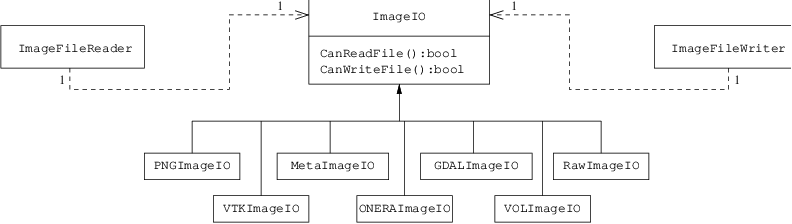
\includegraphics[width=\textwidth]{ImageIOCollaborationDiagram.eps}
\itkcaption[Collaboration diagram of the ImageIO classes]{Collaboration diagram
of the ImageIO classes.} \label{fig:ImageIOCollaborationDiagram}
\end{figure}

\begin{figure}
\center
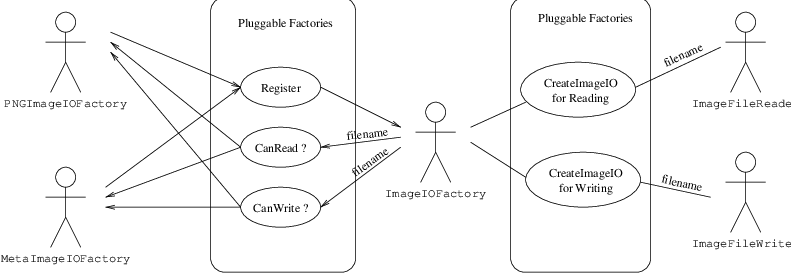
\includegraphics[width=\textwidth]{ImageIOFactoriesUseCases.eps}
\itkcaption[Use cases of ImageIO factories] {Use cases of ImageIO factories.}
\label{fig:ImageIOFactoriesUseCases}
\end{figure}

\begin{figure}
\center
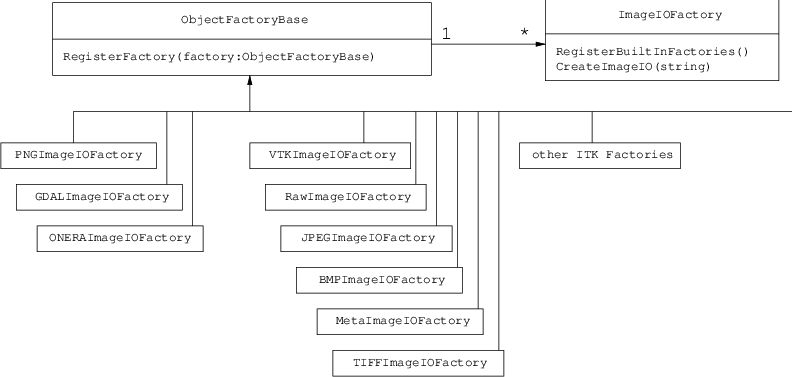
\includegraphics[width=\textwidth]{ImageIOFactoriesClassDiagram.eps}
\itkcaption[Class diagram of ImageIO factories] {Class diagram of the ImageIO
factories.}
\label{fig:ImageIOFactoriesClassDiagram}
\end{figure}


The following section describes the internals of the IO architecture provided
in the toolbox.

\section{Reading, Casting and Writing Images}
\label{sec:ImagReadCastWrite}
\input{ImageReadCastWrite.tex}

\section{Extracting Regions}
\label{sec:ImagReadRegionOfInterestWrite}
\input{ImageReadRegionOfInterestWrite.tex}


\section{Reading and Writing Vector Images}
\index{Image!Multispectral}
\label{sec:VectorImagReadWrite}

Images whose pixel type is a Vector, a CovariantVector, an Array, or a Complex
are quite common in image processing. One of the uses of these tye of
images is the processing of SLC SAR images, which are complex.


\subsection{Reading and Writing Complex Images}
\label{sec:ComplexImagReadWrite}
\input{ComplexImageReadWrite.tex}

\section{Reading and Writing Multiband Images}
\label{sec:MultibandImagReadWrite}
\input{MultibandImageReadWrite.tex}

\subsection{Extracting ROIs}
\label{sec:ExtractROI}
\input{ExtractROI.tex}

\section{Reading Image Series}
\label{sec:ReadingImageSeries}
\input{ImageSeriesIOExample}


\chapter{Reading and Writing Auxiliary Data}
\index{Auxiliary data}
\label{sec:ReadingAuxData}

As we have seen in the previous chapter, OTB has a great capability to
read and process images. However, images are not the only type of data
we will need to manipulate. Images are characterized by a regular
sampling grid. For some data, such as Digital Elevation Models (DEM)
or Lidar, this is too restrictive and we need other representations.

Vector data are also used to represent cartographic objects,
segmentation results, etc: basically, everything which can be seen as
points, lines or polygons. OTB provides functionnalities for accessing
this kind of data.

\section{Reading DEM Files}
\index{Digital elevation model}
\label{sec:ReadDEM}
\input{DEMToImageGenerator.tex}

\section{Elevation management with OTB}
\ifitkFullVersion
\label{sec:DEMHandler}
\fi
\input{DEMHandlerExample.tex}

More examples about representing DEM are presented in section~\ref{sec:ViewingAltitudeImages}.

\section{Reading and Writing Shapefiles and KML}
\index{Auxiliary data!vector data}
\index{Auxiliary data!shapefile}
\index{Auxiliary data!KML}
\label{sec:ReadVectorData}
\input{VectorDataIOExample.tex}


\chapter{Basic Filtering}


This chapter introduces the most commonly used filters found in OTB.
Most of these filters are intended to process images. They will accept one or
more images as input and will produce one or more images as output. OTB is
based ITK's data pipeline architecture in which the output of one filter is
passed as input to another filter. (See Section
\ref{sec:DataProcessingPipeline} on page \pageref{sec:DataProcessingPipeline}
for more information.)


\section{Thresholding}
\ifitkFullVersion
\label{sec:ThresholdingFiltering}
\fi

The thresholding operation is used to change or identify pixel values based
on specifying one or more values (called the \emph{threshold} value). The
following sections describe how to perform thresholding operations using
OTB.

\subsection{Threshold to Point Set}
\label{sec:ThresholdImageToPointSetFilter}

\ifitkFullVersion
\input{ThresholdToPointSetExample.tex}
\fi



\section{Mathematical operations on images}
OTB and ITK provide a lot of filters allowing to perform basic operations on image layers (thresholding, ratio, layers combinations...).
It allows to create a processing chain defining at each step operations and to combine them in the data pipeline.
But the library offers also the possibility to perform more generic complex mathematical operation on images in a single filter: the
\doxygen{otb}{BandMathImageFilter} and more recently the \doxygen{otb}{BandMathImageFilterX}.

\subsection{BandMath filter}
\label{sec:BandMathImageFilter}

\ifitkFullVersion
\input{BandMathFilterExample.tex}
\fi

\subsection{BandMathX filter}
\label{sec:BandMathImageFilterX}
A new version of the BandMath filter is now available; among the new functionalities, variables representing multi-band pixels were introduced, as well as variables representing neighborhoods of pixels. The class name is \doxygen{otb}{BandMathImageFilterX}.

\ifitkFullVersion
\input{BandMathXImageFilterExample.tex}
\fi


\subsection{Ratio of Means Detector}
\input{TouziEdgeDetectorExample}


\subsubsection{Mean Shift filtering and clustering}
\label{sec:MeanShift}

\ifitkFullVersion
\input{MeanShiftSegmentationFilterExample.tex}
\fi



\subsection{Edge Preserving Speckle Reduction Filters}
\label{sec:SpeckleFilters}
\ifitkFullVersion
\input{LeeImageFilter.tex}
\input{FrostImageFilter.tex}
\fi



\subsection{Edge preserving Markov Random Field}

The Markov Random Field framework for OTB is more detailed in \ref{sec:MarkovRandomFieldOTB} (p. \pageref{sec:MarkovRandomFieldOTB}).

\index{Markov!Filtering}
\index{Markov!Restoration}
\ifitkFullVersion
\input{MarkovRestorationExample.tex}
\fi






\input{ImageRegistration.tex}
\chapter{Disparity Map Estimation}
\label{sec:DisparityMapEstimation}

This chapter introduces the tools available in OTB for the estimation
of geometric disparities between images.


\section{Disparity Maps}
\ifitkFullVersion
\label{sec:DisparityMaps}
\fi

The problem we want to deal with is the one of the
automatic disparity map estimation of images acquired with different sensors. By different
sensors, we mean sensors which produce images with different
radiometric properties, that is, sensors which measure different
physical magnitudes: optical sensors operating in different spectral
bands, radar and optical sensors, etc.\\

For this kind of image pairs, the classical approach of fine
correlation \cite{correl1,correl2}, can not always be used to
provide the required accuracy, since this similarity measure (the correlation
coefficient) can only measure similarities up to an affine
transformation of the radiometries.\\

There are two main questions which can be asked about what we want to
do:
\begin{enumerate}
\item Can we define what the similarity is between, for instance, a radar
and an optical image?
\item What does {\em fine registration} mean in the case where the
geometric distortions are so big and the source of information can be
located in different places (for instance, the same edge can be
produced by the edge of the roof of a building in an optical image and
by the wall-ground bounce in a radar image)?
\end{enumerate}

We can answer by saying that the images of the same object obtained by different
sensors are two different representations of the same reality. For the
same spatial location, we have two different measures. Both information
come from the same source and thus they have a lot of common
information. This relationship may not be perfect, but it can be
evaluated in a relative way: different geometrical distortions are
compared and the one leading to the strongest link between the two
measures is kept.\\

%% proposed by Ventura et al. \cite{ventura}. They even applied it to the
%% problem of image to map registration. The approach was also finding HP
%% by matching extracted features.\\


%% Dai and Khorram \cite{xiaolong} use a feature based approach: they
%% extract closed edges which are characterized using invariant
%% moments. Then, the extracted areas are matched using their
%% characterization. Finally, the centers of gravity of each area are
%% used as HP for the estimation of an affine transformation. They apply
%% the approach to Landsat images and they obtain an accuracy better than
%% one pixel, which is similar to the accuracy obtained with manual registration.\\

%% Djamdji et al. \cite{djamdji} propose a multiresolution approach where
%% the discrete wavelet transform is used. The automatic extraction of
%% HP is done by comparing thresholded wavelet coefficients.\\

%% All these approaches try to extract HP in order to
%% compute an analytical deformation model. On the other hand,
When
working with images acquired with the same (type of) sensor one can
use a very effective approach. Since a correlation coefficient measure
is robust and fast for similar images, one can afford to apply it in
every pixel of one image in order to search for the corresponding
HP in the other image. One can thus build a deformation
grid (a sampling of the deformation map). If the sampling step of this grid is short enough, the
interpolation using an analytical model is not needed and high
frequency deformations can be estimated. The obtained grid can be used
as a re-sampling grid and thus obtain the registered images.\\

No doubt, this approach, combined with image interpolation techniques
(in order to estimate sub-pixel deformations) and multi-resolution
strategies allows for obtaining the best performances in terms of
deformation estimation, and hence for the automatic image
registration.\\

Unfortunately, in the multi-sensor case, the correlation coefficient
can not be used. We will thus try to find similarity measures which can be
applied in the multi-sensor case with the same approach as the
correlation coefficient.\\

%% \section{Model for the image registration problem\label{model}}
%% In this section,
We start by giving several definitions which allow for the
formalization of the image registration problem. First of all, we
define the master image and the slave image:
\begin{defin}
Master image: image to which other images will be registered; its
geometry is considered as the reference.
\end{defin}

\begin{defin}
Slave image: image to be geometrically transformed in order to be
registered to the master image.
\end{defin}

Two main concepts are the one of {\em similarity measure} and the one
of {\em geometric transformation}:
\begin{defin}
\label{def-simil}Let $I$ and $J$ be two images and let $c$ a similarity
criterion, we call similarity measure any scalar, strictly positive function 
\begin{equation}
S_c(I,J) = f(I,J,c).
\end{equation}

$S_c$ has an absolute maximum when the two images $I$ and $J$
are {\it identical} in the sense of the criterion $c$.\\
\end{defin}

\begin{defin}\label{defin-T}
A geometric transformation $T$ is an operator which, applied to the
coordinates $(x,y)$ of a point in the slave image, gives the
coordinates $(u,v)$ of its HP in the master image:

\begin{equation}
\left( \begin{array}{c}
u\\
v\\
\end{array}\right) = T \left( \begin{array}{c}
x\\
y\\
\end{array}\right)
\label{Tgeom}
\end{equation}

\end{defin}

Finally we introduce a definition for the image registration problem:
\begin{defin}\label{defin-recal}
Registration problem: \begin{enumerate}
\item determine a geometric transformation $T$ which maximizes the
similarity between a master image $I$ and the result of the
transformation $T\circ J$:
\begin{equation}
Arg \max_T(S_c(I,T\circ J));
\end{equation}
\item re-sampling of $J$ by applying $T$.
\end{enumerate}

\end{defin}

%% We must note that Le Moigne et al. have proposed in a recent contribution
%% \cite{ig02lemoigne} a modular approach for the
%% registration which allows the analysis of different similarity
%% measures and different optimization strategies. The presented results,
%% which are still preliminary, are very promising. The multi-sensor
%% case has been dealt with, but only for optical images (Ikonos and
%% Landsat/ETM+). The case of very different images (for instance optical
%% and radar) has not been explored.\\


\subsection{Geometric deformation modeling\label{sec-model}}
The geometric transformation of definition \ref{defin-T} is used for
the correction of the existing deformation between the two images to be
registered. This deformation contains information which are linked to
the observed scene and the acquisition conditions. They
can be classified into 3 classes depending on their physical source:
\begin{enumerate}
\item deformations linked to the mean attitude of the sensor
(incidence angle, presence or absence of yaw steering, etc.);
\item deformations linked to a stereo vision (mainly due to the topography);
\item deformations linked to attitude evolution during the acquisition
(vibrations which are mainly present in push-broom sensors).
\end{enumerate}

These deformations are characterized by their spatial frequencies and
intensities which are summarized in table \ref{tab-deform}.\\

\begin{table}[b]
\begin{center}
\begin{tabular}{|c|c|c|}
\hline
& Intensity & Spatial Frequency\\
\hline
Mean Attitude & Strong & Low \\
\hline
Stereo & Medium & High and Medium\\
\hline
Attitude evolution & Low & Low to Medium \\
\hline
\end{tabular}
\end{center}
\caption{Characterization of the geometric deformation sources}
\label{tab-deform}
\end{table}

Depending on the type of deformation to be corrected, its model will be
different. For example, if the only deformation to be corrected is the
one introduced by the mean attitude, a physical model for the
acquisition geometry (independent of the image contents) will be
enough. If the sensor is not well known, this deformation can be
approximated by a simple analytical model. When the deformations to be
modeled are high frequency, analytical (parametric) models are not
suitable for a fine registration. In this case, one has to use a fine
sampling of the deformation, that means the use of deformation
grids. These grids give, for a set of pixels of the master image,
their location in the slave image.\\

The following points summarize the problem of the deformation modeling:
\begin{enumerate}
\item An analytical model is just an approximation of the
deformation. It is often obtained as follows:
\begin{enumerate}
\item Directly from a physical model without using any image content information.
\item By estimation of the parameters of an a priori model
(polynomial, affine, etc.). These parameters can be estimated:
\begin{enumerate}
\item Either by solving the equations obtained by taking HP. The HP can be manually or automatically extracted.
\item Or by maximization of a global similarity measure.
\end{enumerate}

\end{enumerate}
\item A deformation grid is a sampling of the deformation map.
\end{enumerate}

The last point implies that the sampling period of the grid must be short
enough in order to account for high frequency deformations (Shannon
theorem). Of course, if the deformations are non stationary (it is
usually the case of topographic deformations), the sampling can 
be irregular.\\

As a conclusion, we can say that definition \ref{defin-recal} poses
the registration problem as an optimization problem. This optimization
can be either global or local with a similarity measure which can also
be either local or global. All this is synthesized in table  \ref{tab-approches}.\\

\begin{table}[b]
\begin{center}
\begin{tabular}{|c|c|c|}
\hline
Geometric model & Similarity measure & Optimization of the \\
& & deformation \\
\hline
Physical model & None & Global \\
\hline
Analytical model  & Local & Global \\
with a priori HP & & \\
\hline
Analytical model& Global & Global \\
without a priori HP & & \\
\hline
Grid & Local & Local \\
\hline
\end{tabular}
\end{center}
\caption{Approaches to image registration}
\label{tab-approches}
\end{table}

The ideal approach would consist in a registration which is locally
optimized, both in similarity and deformation, in order to have the
best registration quality. This is the case when deformation grids with
dense sampling are used. Unfortunately, this case is the most
computationally heavy and one often uses either a low sampling rate of
the grid, or the evaluation of the similarity in a small set of pixels
for the estimation of an analytical model. Both of these choices lead to local registration
errors which, depending on the topography, can amount several
pixels.\\

Even if this registration accuracy can be enough in many
applications, (ortho-registration, import into a GIS, etc.), it is not
acceptable in the case of data fusion, multi-channel segmentation or
change detection \cite{townshend}. This is why we will focus on the
problem of deformation estimation using dense grids.\\

%% None of the references presented in section \ref{review} uses the
%% local optimization approach. We can also note that in the multi-sensor
%% case only few authors \cite{ig02lemoigne} have used any similarity
%% measure other than the correlation coefficient. However, in the
%% medical imaging field, as we will see in section \ref{sec-simil}, a
%% lot of similarity measures have been proposed as a generalization of
%% the correlation coefficient. These measures enable the registration of
%% very different imagery modalities. Nevertheless, these works are not
%% directly usable in our problem since the geometric deformations
%% present in medical images can be easily represented by global
%% analytical models. Indeed, often a rigid model (rotation, translation,
%% scale) or slightly elastic (affine plus a $a\cdot x\cdot y$ term) is
%% enough since the sensors are stable, the stereo effect is small and
%% only the point of view changes. As we have noted above, deformations
%% due to topography can locally have high frequencies for medium and
%% high resolution sensors (30 m. and better), thus our need for a fine
%% modeling. We also point out that the problem of hidden faces is beyond
%% the scope of this paper.\\


\subsection{Similarity measures\label{sec-simil}}


The fine modeling of the geometric deformation we are looking for
needs for the estimation of the coordinates of nearly every pixel in
the master image inside the slave image. In the classical mono-sensor
case where we use the correlation coefficient we proceed as follows.\\

The geometric deformation is modeled by local rigid displacements. One
wants to estimate the coordinates of each pixel of the master image inside the
slave image. This can be represented by a displacement vector
associated to every pixel of the master image. Each of the two components
(lines and columns) of this vector field will be called deformation grid.\\

We use a small window taken in the master image and we test the similarity
for every possible shift within an exploration area inside the slave
image (figure \ref{zones}). \\

\begin{figure}
%\begin{center}{\includegraphics[width=0.8\hsize]{zones.eps}}
  \begin{center}
    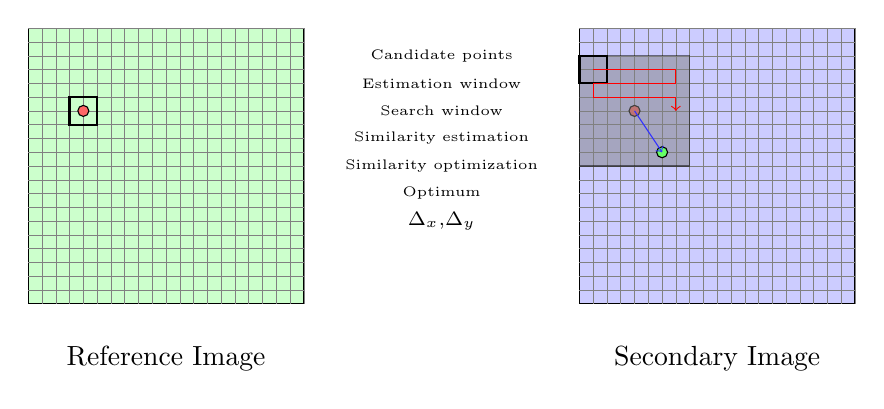
\begin{tikzpicture}[scale=0.35]
    \draw[fill=green!20] (5,5) rectangle (15,15);
    \draw[step=0.5, gray, very thin] (5,5) grid (15,15);
    \node (Reference) at (10,3) {Reference Image};

    \draw[fill=blue!20] (25,5) rectangle (35,15);
    \draw[step=0.5, gray, very thin] (25,5) grid (35,15);
    \node (Reference) at (30,3) {Secondary Image};
    
    \draw[fill=red!60] (7,12) circle (0.2);
    \draw[fill=red!60] (27,12) circle (0.2);
    \node (CPs) at (20,14) {\tiny Candidate points};
    
    \draw[thick] (6.5,11.5) rectangle +(1,1);
    \node (EW) at (20,13) {\tiny Estimation window};
    
    \draw[fill=gray, opacity=0.5] (25,10) rectangle +(4,4);
    \node (SW) at (20,12) {\tiny Search window};
    
    \draw[thick] (25,13) rectangle +(1,1);
    \node (SEW) at (20,11) {\tiny Similarity estimation};
    
    \draw[red,->] (25.5,13.5) --  ++(3,0) -- ++(0,-0.5) -- ++(-3,0) -- ++(0,-0.5) --++(3,0) -- ++(0,-0.5)  ;
    \node (OPT) at (20,10) {\tiny Similarity optimization};
    
    \draw[fill=green!60] (28,10.5) circle (0.2);
    \node (OPTF) at (20,9) {\tiny Optimum};
    
    \draw[blue!80,->] (27,12) -- (28,10.5);
    \node (Deltas) at (20,8) {$\scriptstyle{\Delta_x,\Delta_y}$};
    
  \end{tikzpicture}
    \end{center}
\caption{Estimation of the correlation surface.}
\label{zones}
\end{figure}


That means that for each position we compute the correlation
coefficient. The result is a correlation surface whose
maximum gives the most likely local shift between both images:

\begin{equation}
\begin{split}
&\rho_{I,J}(\Delta x, \Delta y) = \\
&\frac{1}{N}\frac{\sum_{x,y}(I(x,y)-m_I)(J(x+\Delta x,y+\Delta y)-m_J)}{\sigma_I
\sigma_J}.
\end{split}
\end{equation}

In this expression, $N$ is the number of pixels of the analysis
window, $m_I$ and $m_J$ are the estimated mean values inside the
analysis window of respectively image $I$ and image $J$ and $\sigma_I$
and $\sigma_J$ are their standard deviations.\\

Quality criteria can be applied to the estimated maximum in order to
 give a confidence factor to the estimated shift: width of the peak,
 maximum value, etc. Sub-pixel shifts can be measured by applying
 fractional shifts to the sliding window. This can be done by image interpolation.\\

The interesting parameters of the procedure are:
\begin{itemize}
\item The size of the exploration area: it determines the
computational load of the algorithm (we want to reduce it), but it has
to be large enough in order to cope with large deformations.
\item The size of the sliding window: the robustness of the correlation
coefficient estimation increases with the window size, but the
hypothesis of local rigid shifts may not be valid for large windows.
\end{itemize}

The correlation coefficient cannot be used with original grey-level
images in the multi-sensor case. It could be used on extracted
features (edges, etc.), but the feature extraction can introduce
localization errors. Also, when the images come from sensors using
very different modalities, it can be difficult to find similar
features in both images. In this case, one can try to find the
similarity at the pixel level, but with other similarity measures and
apply the same approach as we have just described.\\

The concept of similarity measure has been presented in definition
\ref{def-simil}. The difficulty of the procedure lies in finding the
function $f$ which properly represents the criterion $c$. We also need
that $f$ be easily and robustly estimated with small windows. We extend here what we proposed in \cite{ig02simil}.\\

\subsection{The correlation coefficient\label{expe}}
We remind here the computation of the correlation coefficient between
two image windows $I$ and $J$. The coordinates of the pixels inside
the windows are represented by $(x,y)$:

\begin{equation}
\rho(I,J) = \frac{1}{N}\frac{\sum_{x,y}(I(x,y)-m_I)(J(x,y)-m_J)}{\sigma_I
\sigma_J}.
\label{coeffcorr}
\end{equation}

In order to qualitatively characterize the different similarity
measures we propose the following experiment. We take two images which
are perfectly registered and we extract a small window
of size $N\times M$ from each of the images (this size is set to
$101\times 101$ for this experiment). For the master image, the
window will be centered on coordinates $(x_0,
y_0)$ (the center of the image) and for the slave image, it will be centered on coordinates $(x_0+\Delta x,
y_0)$. With different values of $\Delta x$ (from -10 pixels to 10
pixels in our experiments), we obtain an estimate of $\rho(I,J)$ as a
function of $\Delta x$, which we write as
$\rho(\Delta x)$ for short. The obtained curve should have a maximum for
$\Delta x =0$, since the images are perfectly registered. We would
also like to have an absolute maximum with a high value and with a
sharp peak, in order to have a good precision for the shift estimate.\\

%% In the following, we will make this experiment with different image
%% pairs and different similarity measures. Figure \ref{fig-correl}
%% shows the results obtained when the correlation coefficient is applied
%%  to (\ref{correl-B1B1}) one extract of the B1 channel of a Spot 5
%% image with itself, (\ref{correl-B1B3}) an extract of channel B1 with the
%% extract of channel B3,  and (\ref{correl-B1ERS}) the extract of
%% channel B1 with an
%% extract of an ERS-2 SAR image. The images are presented in figures
%% \ref{histo_b1_b1}, \ref{histo_b1_b3} and \ref{histo_b1_ers}.\\


%% % \begin{figure*}
%% % \centerline{\subfigure[Correlation B1-B1]{\includegraphics[width=0.5\hsize]{CORREL_b1_b1_10.pdf}\label{correl-B1B1}} \\
%% % \subfigure[Correlation
%% % B1-B3]{\includegraphics[width=0.5\hsize]{CORREL_b1_b3_10.pdf}\label{correl-B1B3}}\\
%% % \subfigure[Correlation B1-ERS]{\includegraphics[width=0.5\hsize]{CORREL_b1_ERS_10_0.pdf}\label{correl-B1ERS}}}
%% % \caption{Measure of $\rho(\Delta x)$ for 3 different pairs of images.}
%% % \label{fig-correl}
%% % \end{figure*}

%% \begin{figure*}
%% \centering
%% \subfigure[Correlation B1-B1]{\includegraphics[width=0.4\hsize]{CORREL_b1_b1_10.pdf}\label{correl-B1B1}} \\
%% \subfigure[Correlation
%% B1-B3]{\includegraphics[width=0.4\hsize]{CORREL_b1_b3_10.pdf}\label{correl-B1B3}}\\
%% \subfigure[Correlation B1-ERS]{\includegraphics[width=0.4\hsize]{CORREL_b1_ERS_10_0.pdf}\label{correl-B1ERS}}
%% \caption{Measure of $\rho(\Delta x)$ for 3 different pairs of images.}
%% \label{fig-correl}
%% \end{figure*}

%% We can see that the correlation coefficient has a good behavior for
%% the first pair, but its performances are bad when the images
%% radiometries are different. The correlation coefficient
%%  can be characterized as follows:
%% \begin{itemize}
%% \item Well known algorithm.
%% \item Fits the registration needs when using radiometrically similar images.
%% \item Simple and fast computation.
%% \item High precision in the estimation of the deformation.
%% \item Robust to noise.
%% \end{itemize}

%% However its main disadvantage is that it can only take into account
%%  affine transformations between radiometries ($j = \alpha i + \beta$)
%%  so it can not be used in the general multi-sensor case.\\


%% \subsection{Generalization: probabilistic interpretation \label{sec_correl}}
%% The correlation coefficient formulation (equation \ref{coeffcorr}) can
%% be revisited with a probabilistic interpretation:

%% \begin{equation}
%% \begin{split}
%% \rho(I,J) &= \frac{1}{N}\frac{\sum_{x,y}(I(x,y)-m_I)(J(x,y)-m_J)}{\sigma_I
%% \sigma_J} \\
%% &= \sum_{(i,j)}\frac{(i-m_I)(j-m_J)}{\sigma_I \sigma_J}p_{ij}
%% \end{split}
%% \label{coeffcorr2}
%% \end{equation}

%% where the sum is taken over the list of radiometry pairs $(i,j)$, and
%% $p_{ij}$ is the value of the joint normalized histogram (estimation of
%% the joint probability density function, pdf, $f_{ij}(i,j)$) of the pair of images.\\

%% That means that we are assuming a linear model
%% \begin{equation}
%% j = (i-m_I)\frac{\sigma_J}{\sigma_I}+m_J,
%% \end{equation}
%% and we evaluate its likelihood by weighting with the probability of
%% each radiometry couple, $p_{ij}$.\\

%% One could assume different models for the radiometry pairs leading to
%% different measures as, for instance, the identity model , $i=j$, which
%% leads to the $L_n$ norm:

%% \begin{equation}
%% L_n(I,J) = \sum_{i,j} \left| i - j\right|^n p_{ij},
%% \end{equation}

%% or more complex models based on textural approaches :

%% Diagonal moment:
%% \begin{equation}
%% MD(I,J) = \sum_{i,j}\left| i - j\right|(i+j-\sigma_I-\sigma_J) p_{ij},
%% \end{equation}

%%  Cluster Shade:
%% \begin{equation}
%% C_{shade}(I,J) = \sum_{i,j} (i+j-\sigma_I-\sigma_J)^3 p_{ij},
%% \end{equation}

%%  Cluster Prominence:
%% \begin{equation}
%% C_{pro}(I,J) = \sum_{i,j} (i+j-\sigma_I-\sigma_J)^4 p_{ij}.
%% \end{equation}

%% An assessment of these measures for image registration can be found in
%% \cite{bro}. They are very sensitive to noise and are not useful for
%% the comparison of grey-levels of multi-sensor image pairs.\\

%% \subsection{Estimation of similarity measures and $p_{IJ}$}

%% In the expression of the correlation coefficient the term $p_{ij}$ is
%% an estimation of the joint pdf of the radiometries of
%% the images we are comparing. It can be seen as a link (transfer
%% function) between both radiometries.\\

%% % We want a measure of the
%% % similarity measure which is valid locally, that is, which takes into
%% % account the specificities of the neighborhood of the pixel for which
%% % we are estimating the deformation. That means that we have to use a
%% % small estimation window around the pixel of interest. On the other
%% % hand, we want a robust estimate, thus we need reliable values of
%% % $p_{ij}$, which means the use of a high number of samples.\\


%% %\subsubsection{Examples of $p_{ij}$ estimation}

%% We show here several examples of the estimation of the joint
%% histogram. On figures \ref{histo_b1_b1}, \ref{histo_b1_b3} and
%% \ref{histo_b1_ers} are shown respectively the joint histograms of one
%% image with itself (B1-B1), two different channels of the same Spot 5
%% image (B1-B3) and a Spot 5 B3 - ERS-2 pair.\\

%% \begin{figure}
%% \centering
%% \subfigure[SPOT 5 B1]{\includegraphics[width=0.5\hsize]{b1_1980_1980.pdf}} \\
%% \subfigure[Joint histogram]{\includegraphics[width=0.5\hsize]{hb1.pdf}}
%% \caption{Joint histogram of an image with itself.}
%% \label{histo_b1_b1}
%% \end{figure}


%% \begin{figure}
%% \centering
%% \subfigure[SPOT 5 B1]{\includegraphics[width=0.5\hsize]{b1_3376_3882.pdf}}\\
%% \subfigure[SPOT 5 B3]{\includegraphics[width=0.5\hsize]{b3_3376_3882.pdf}}\\
%% \subfigure[Joint histogram]{\includegraphics[width=0.5\hsize]{hb3.pdf}}\\
%% \caption{Joint histogram of two channels (B1-B3) of the same Spot 5 image.}
%% \label{histo_b1_b3}
%% \end{figure}



%% \begin{figure}
%% \centering
%% \subfigure[SPOT 5 B3]{\includegraphics[width=0.5\hsize]{b1_1500_2500.pdf}}\\
%% \subfigure[ERS-2]{\includegraphics[width=0.5\hsize]{ERS_1500_2500.pdf}}\\
%% \subfigure[Joint histogram]{\includegraphics[width=0.5\hsize]{hers.pdf}}\\
%% \caption{Joint histogram of a Spot 5 B3 image and a ERS-2 image.}
%% \label{histo_b1_ers}
%% \end{figure}

%% As expected, the joint histogram of an image with itself is a straight
%% line with slope 1. It shows the full correlation between the two
%% images: the identity transfer function. This kind of situation is well
%% dealt with by the correlation coefficient.\\

%% The B1-B3 case (figure \ref{histo_b1_b3}) shows two nearly linear tendencies which are
%% mixed up. This case can not be dealt with by the correlation coefficient.\\

%% Finally, figure \ref{histo_b1_ers} shows the impossibility of finding
%% any correlation link between two sensors which are as different as an
%% optical and a radar one.\\


%% \subsubsection{Computation time}
%% The main difference between the two expressions of the correlation
%% coefficient given by equations \ref{coeffcorr} and \ref{coeffcorr2} is
%% the estimation of the joint pdf needed in the second
%% expression. This estimation is usually done by computing the joint
%% histogram. The joint histogram can be computed with different methods,
%% but their discussion is beyond the scope of this paper. However it is
%% important to note that the method chosen for histogram computation may
%% induce significative changes in the computation cost of the similarity
%% measure. As an example, with our implementation (counting with
%% optimization of the number of classes) there is an increase factor of 4 in
%% computation time between equation \ref{coeffcorr} and equation
%% \ref{coeffcorr2}.\\

%% The multi-sensor measures which will be introduced in the next section
%% need the estimation of the joint histogram. Hence, their computation
%% time is comparable to the one of equation \ref{coeffcorr2}. The
%% differences of computation complexity between these measures are
%% negligible, since the longest part of the algorithm is taken by the
%% joint histogram estimation.\\


%% \subsection{Multi-sensor measures.}
%% We introduce here several similarity measures which have been proved
%% useful in the problem of multi-modality medical image registration \cite{dsarrut-thesis}.\\

%% In the following, the sums will be computed over radiometry values. We
%% will use the conditional mean:
%% \begin{equation}
%% m_{I|j} = \frac{1}{p_j}\sum_i i p_{ij};
%% \end{equation}

%% and the conditional variance:

%% \begin{equation}
%% \sigma^2_{I|j} = \frac{1}{p_j}\sum_i (i-m_{I|j})^2 p_{ij}.
%% \end{equation}

%% For each of the following measures, we will perform the experiment
%% described in section \ref{expe}.\\


%% \subsubsection{Measures using the radiometry values and the probabilities}

%% Within this class, we will not take into account the measures which
%% are based on the differences of radiometries ($L_n$ norm of the
%% difference) \cite{tru98,cm87,akn89}, or textural measures, since they
%% give low quality results.\\


%% \paragraph{Normalised standard deviation or Woods criterion}

%% The work by Woods et al. first on mono-modal registration 
%% \cite{wcm92} and then on multi-modal registration \cite{wmc93} lead to
%% the elaboration of this similarity measure. Given the intensity on one
%% image, that is the set of pixels having this value, this measure takes
%% into account the variability of the intensities of the homologous
%% pixels in the other image. The underlying hypothesis is that this
%% variability (which is actually a measure of variance) will be minimum
%% when the images are registered:

%% \begin{equation}
%% Woods(I|J) = \sum_j \frac{\sigma_{I|j}}{m_{I|j}}p_j
%% \end{equation}

%% In order to have a criterion which has to be maximised, we will use:
%% \begin{equation}
%% S_{Woods}(I|J) = 1-\sum_j \frac{\sigma_{I|j}}{m_{I|j}}p_j
%% \end{equation}

%% The results on our three test image pairs are shown in figure
%% \ref{woods}. We see that for the mono-sensor case the results are
%% similar to those of the correlation coefficient. For the two
%% multi-sensor examples, we obtain high values near the 0-shift, but the
%% location of these maxima is not accurate.\\

%% \begin{figure*}
%% \centering
%% \subfigure[B1 with B1]{\includegraphics[width=0.4\hsize]{WOODS_b1_b1_1_60_15.pdf}}\\
%% \subfigure[B1 with B3]{\includegraphics[width=0.4\hsize]{WOODS_b1_b3_1_60_15.pdf}}\\
%% \subfigure[B1 with ERS]{\includegraphics[width=0.4\hsize]{WOODS_b1_ERS_60_15_0.pdf}}
%% \caption{Image shift experiment: Woods criterion.}
%% \label{woods}
%% \end{figure*}


%% \paragraph{Correlation ratio}

%% This is a very well known measure in statistics. It has been first
%% proposed in the framework of image registration by Roche et
%% al. \cite{rmpa98b}. It is defined as follows:
%% \begin{equation}
%% \eta^2(I|J) = 1-\frac{1}{\sigma_I^2}\sum_j \sigma_{I|j}^2p_j
%% \end{equation}

%% Its interpretation is similar to the one of the Woods criterion. The
%% results are shown in figure \ref{rapcorr} and they are worse than
%% those of the Woods criterion.\\

%% \begin{figure*}
%% \centering
%% \subfigure[B1 with B1]{\includegraphics[width=0.4\hsize]{RAPCORR_b1_b1_0_80_10.pdf}}\\
%% \subfigure[B1 with B3]{\includegraphics[width=0.4\hsize]{RAPCORR_b1_b3_1_60_10.pdf}}\\
%% \subfigure[B1 with ERS]{\includegraphics[width=0.4\hsize]{RAPCORR_b1_ERS_80_10_0.pdf}}
%% \caption{Image shift experiment: Correlation ratio.}
%% \label{rapcorr}
%% \end{figure*}

%% \subsubsection{Measures using only the probabilities}

%% This class of measures does not directly use the radiometries of the
%% pixels, but only the estimation of the joint pdf. Of course,
%% the pixel pairs are used for the estimation of this probability.\\


%% \paragraph{Distance to independence}

%% It is a normalised version of the $\chi^2$ test:
%% \begin{equation}
%% \chi^2(I,J) = \sum_{i,j}\frac{(p_{ij}-p_i p_j)^2}{p_i p_j}
%% \end{equation}

%% It measures the degree of statistical dependence between both images,
%% since for two independent random variables, the joint pdf is
%% equal to the product of the marginals. The correlation coefficient is
%% a test of independence of order 2 and this one is the generalisation
%% to any order. The results are shown in figure \ref{chi2}. In this
%% case, for the three pairs, we obtain an absolute maximum for the
%% 0-shift case which is sharp enough for a robust automatic detection.\\

%% \begin{figure*}
%% \centering
%% \subfigure[B1 with B1]{\includegraphics[width=0.4\hsize]{KI2_b1_b1_0_100_5.pdf}}\\
%% \subfigure[B1 with B3]{\includegraphics[width=0.4\hsize]{KI2_b1_b3_1_100_5.pdf}}\\
%% \subfigure[B1 with ERS]{\includegraphics[width=0.4\hsize]{KI2_b1_ERS_100_5_0.pdf}}
%% \caption{Image shift experiment: Distance to independence.}
%% \label{chi2}
%% \end{figure*}


%% \paragraph{The $f-divergence$ family}
%% A $f-divergence$ \cite{csiszar} measures the expectation of the
%% diversity of the likelihood ratio between two distributions $P$ and $Q$:

%% \begin{equation}
%% \begin{split}
%% D_{f}(P,Q) = E_Q \left[f\left( \frac{d p(x)}{d q(x)} \right)\right] 
%% =  \int f\left(\frac{p(x)}{q(x)}\right)q(x) dx
%% \end{split}
%% \end{equation}

%% $E_Q$ is the expectation with respect to $Q$, $\frac{d p(x)}{d q(x)}$
%% is the derivative with respect to a density, 
%% $f$ is continuous and convex on $[0,+\infty)$. A divergence can be
%% seen as a relative entropy. In order to simplify the
%% notation, we will use: $p=p_{ij}$, $q=p_i p_j$, $\int = \sum_{i,j}$.\\


%% \begin{table}[b]
%% \begin{center}
%% \begin{tabular}{|c|c|}
%% \hlx{hv}
%% Measure & $f(x)$ \\
%% \hlx{hv}
%% Kolmogorov distance & $\frac{1}{2}|x-1|$ \\
%% \hlx{hv}
%% Mutual information & $x\log x$ \\
%% \hlx{hv}
%% Kullback divergence & $(x-1)\log x$ \\
%% \hlx{hv}
%% $\chi^2$-divergence & $\frac{1}{2}(x -1)^2$ \\
%% \hlx{hv}
%% Hellinger distance & $\frac{1}{2}(\sqrt x -1)^2$ \\
%% % \hlx{hv}
%% % Bhattacharyaa distance & $\sqrt x$ \\
%% \hlx{hv}
%% Toussaints distance & $x \frac{x-1}{x+1}$ \\
%% \hlx{hv}
%% Lin K-divergence & $x\log \frac{2x}{1+x}$ \\
%% \hlx{vhs}
%% \end{tabular}
%% \end{center}
%% \caption{Expressions of function $f$ in the $f-divergence$ family.}
%% \label{tabfg}
%% \end{table}

%% Depending on the choice of $f$ (see table \ref{tabfg}), we can obtain several
%% interesting cases:


%% \begin{enumerate}
%% \item Kolmogorov distance:
%% \begin{equation}
%% V(P,Q) = \frac{1}{2} \int\left| p -q\right|
%% \end{equation}


%% \item Kullback information or mutual information:
%% \begin{equation}
%% K(P,Q) = \int p \log\frac{p}{q}
%% \end{equation}


%% \item Kullback divergence:
%% \begin{equation}
%% K'(P,Q) = \int (q-p)\left( \log q - \log p \right)
%% \end{equation}

%% \item $\chi^2$-divergence:
%% \begin{equation}
%% R(P,Q) = \frac{1}{2}\int \frac{(p-q)^2}{q}
%% \end{equation}


%% \item Hellinger distance:
%% \begin{equation}
%% {\cal H}^2 (P,Q) = \frac{1}{2}\int (\sqrt p - \sqrt q)^2
%% \end{equation}

%% % \item Bhattacharyaa distance:
%% % \begin{equation}
%% % {\cal B} (P,Q) = -2 \log\left(\int \sqrt{ p q}\right)
%% % \end{equation}

%% \item Toussaints distance:
%% \begin{equation}
%% T (P,Q) = \int p-\frac{2pq}{p+q}
%% \end{equation}


%% \item Lin K-divergence:
%% \begin{equation}
%% K_{div} (P,Q) = \int p\log \frac{2p}{p+q}
%% \end{equation}

%% \end{enumerate}


%% All these measures give very similar results \cite{sm99}. We study two of them:



%% \begin{enumerate}
%% \item Kolmogorov distance
%% \begin{equation}
%% V(P,Q) = \frac{1}{2} \int\left| p_{ij} -p_i p_j\right|
%% \end{equation}

%% It can be seen as a $L_1$ norm version of the $\chi^2$ criterion. The
%% results are shown in figure \ref{distkol}.\\


%% \begin{figure*}
%% \centering
%% \subfigure[B1 with B1]{\includegraphics[width=0.4\hsize]{DISTKOLM_b1_b1_0_100_5.pdf}}\\
%% \subfigure[B1 with B3]{\includegraphics[width=0.4\hsize]{DISTKOLM_b1_b3_1_100_5.pdf}}\\
%% \subfigure[B1 with ERS]{\includegraphics[width=0.4\hsize]{DISTKOLM_b1_ERS_100_5_0.pdf}}
%% \caption{Image shift experiment: Kolmogorov distance.}
%% \label{distkol}
%% \end{figure*}


%% \item Mutual information
%% \begin{equation}
%% K(P,Q) = \int p_{ij} \log\frac{p_{ij}}{p_i p_j}
%% \end{equation}


%% The results are shown in figure \ref{infokull}.\\


%% \begin{figure*}
%% \centering
%% \subfigure[B1 with B1]{\includegraphics[width=0.4\hsize]{INFKULL_b1_b1_0_100_5.pdf}}\\
%% \subfigure[B1 with B3]{\includegraphics[width=0.4\hsize]{INFKULL_b1_b3_1_100_5.pdf}}\\
%% \subfigure[B1 with ERS]{\includegraphics[width=0.4\hsize]{INFKULL_b1_ERS_100_5_0.pdf}}
%% \caption{Image shift experiment: Mutual information.}
%% \label{infokull}
%% \end{figure*}

%% \end{enumerate}


%% Both measures give satisfactory results which are very similar to the
%% ones obtained with the distance to the independence.\\


%% % \paragraph{Proportional reduction of the prediction error}

%% % It is an extension of the correlation concept to categorial variables
%% %  \cite{shh98,weh96,rmap99}. We measure the ability of a variable to
%% %  predict the other. We define an uncertainty measure $V(I)$ and the
%% %  prediction error is defined as:
%% % \begin{equation}
%% % PRE_V(I|J) = \frac{V(I)-E\left[ V(I|J) \right]}{V(I)}
%% % \end{equation}

%% % This measure can be made symmetric:
%% % \begin{equation}
%% % PRE_V(I,J) = \frac{V(I)+V(J)-E\left[ V(I|J) \right]- E\left[ V(J|I) \right]}{V(I)+V(J)}
%% % \end{equation}

%% % If the uncertainty measure used is the entropy, one can define the
%% % following coefficients:
%% % \begin{equation}
%% % u(I|J) = \frac{H(I)-H(I|J)}{H(I)}=\frac{{\cal I}(I,J)}{H(I)}
%% % \end{equation}

%% % \begin{equation}
%% % k(I,J) = \frac{{\cal I}(I,J)}{H(I)+H(J)}
%% % \end{equation}

%% % \begin{equation}
%% % r(I,J) = \sqrt{1-\left( \frac{{\cal I}(I,J)}{H(I,J)} \right)^2}
%% % \end{equation}

%% % With this same principle and using the variance a s uncertainty
%% %  measure we obtain the correlation ratio:
%% % \begin{equation}
%% % \eta^2(I|J) = \frac{Var(I)-Var(E[I|J])}{Var(I)}
%% % \end{equation}

%% % We detail the results of one of these measures:

%% % \paragraph{U criterion}
%% % \begin{equation}
%% % u(I|J) = \frac{H(I)-H(I|J)}{H(I)}=\frac{{\cal I}(I,J)}{H(I)}
%% % \end{equation}

%% % It measures the the entropy and the conditional entropy. This distance
%% % increases when the two variables are linked. The results on our 3 test
%% % pairs are shown on figure \ref{critereU}.\\


%% % \begin{figure*}
%% % \centerline{\subfigure[B1 with B1]{\includegraphics[width=0.5\hsize]{U_b1_b1_1_40.pdf}}\\
%% % \subfigure[B1 with B3]{\includegraphics[width=0.5\hsize]{U_b1_b3_1_40.pdf}}\\
%% % \subfigure[B1 with ERS]{\includegraphics[width=0.5\hsize]{U_b1_ERS_80_0.pdf}}}
%% % \caption{Image shift experiment: U criterion.}
%% % \label{critereU}
%% % \end{figure*}


%% \paragraph{Cluster reward algorithm}


%% Let $H_{IJ}(k,l)$ be the joint histogram of the pair of images and
%% let  $H_I(k)$ and $H_J(k)$ respectively be the marginal histograms and
%% $P$ the number of pixels. We define 
%% \begin{equation}
%% I_{CRA} = \frac{\frac{\Phi}{F}- \frac{F}{P^2}}{1-\frac{F}{P^2}};
%% \label{cra}
%% \end{equation}
 
%% where
%% \begin{subequations}
%% \begin{equation}
%% \Phi = \sum_{k=0}^{N-1} \sum_{l=0}^{N-1} H_{IJ}^2(k,l);
%% \end{equation}
%% \begin{equation}
%% F=\sqrt{h_I h_J};
%% \end{equation}
%% \begin{equation}
%% h_I = \sum_{k=0}^{N-1} H_{I}^2(k);
%% \end{equation}
%% \begin{equation}
%% h_J = \sum_{k=0}^{N-1} H_{J}^2(k);
%% \end{equation}
%% \end{subequations}

%% The $I_{CRA}$ index will have a high value when the joint histogram
%% has little dispersion. This lack of dispersion can be due to a
%% correlation (histogram distributed along a line) or to the clustering
%% of radiometry values within the histogram. In both cases one can
%% predict the values of one image from the values of the other.\\

%% In order to compare $I_{CRA}$ with the $f-divergences$, we can rewrite equation \ref{cra} as:

%% \begin{equation}
%% I_{CRA} = \frac{\int p_{ij}^2 - \int p_i^2
%% \int p_j^2}{\sqrt{\int p_i^2 \int p_j^2} - \int p_i^2
%% \int p_j^2}.
%% \label{cra2}
%% \end{equation}
%%  If we consider the denominator as a normalization term, we can focus
%% only in the numerator. This numerator contains the same terms as the
%% $f-divergences$, that is, a term which depends on the joint
%% pdf and a term which depends on the product of the
%% marginals. We can thus make an interpretation which is similar to the
%% independence tests. As expected, the obtained results (figure
%% \ref{cra_figure}) are similar to those obtained with the $f-divergences$.\\


%% \begin{figure*}
%% \centering
%% \subfigure[B1 with B1]{\includegraphics[width=0.4\hsize]{K_b1_b1_1_40.pdf}}\\
%% \subfigure[B1 with B3]{\includegraphics[width=0.4\hsize]{K_b1_b3_1_40.pdf}}\\
%% \subfigure[B1 with ERS]{\includegraphics[width=0.4\hsize]{K_b1_ERS_80_0.pdf}}
%% \caption{Image shift experiment: Cluster reward algorithm.}
%% \label{cra_figure}
%% \end{figure*}

%% The main interest of the CRA with respect to the $f-divergence$ family
%% is that the joint histogram noise due to estimation has less influence
%% in the similarity measure. This allows us to use smaller estimation
%% windows. The only drawback in doing this is that the peak of the
%% measure will be less sharp.\\


\section{Regular grid disparity map estimation}
\label{sec:SimpleDisparityMapEstimationDense}
%% \ifitkFullVersion
\input{FineRegistrationImageFilterExample.tex}
%% \fi


\input{StereoReconstruction.tex}
\chapter{Orthorectification and Map Projection}\label{sec:Ortho}


\begin{figure}[h]
  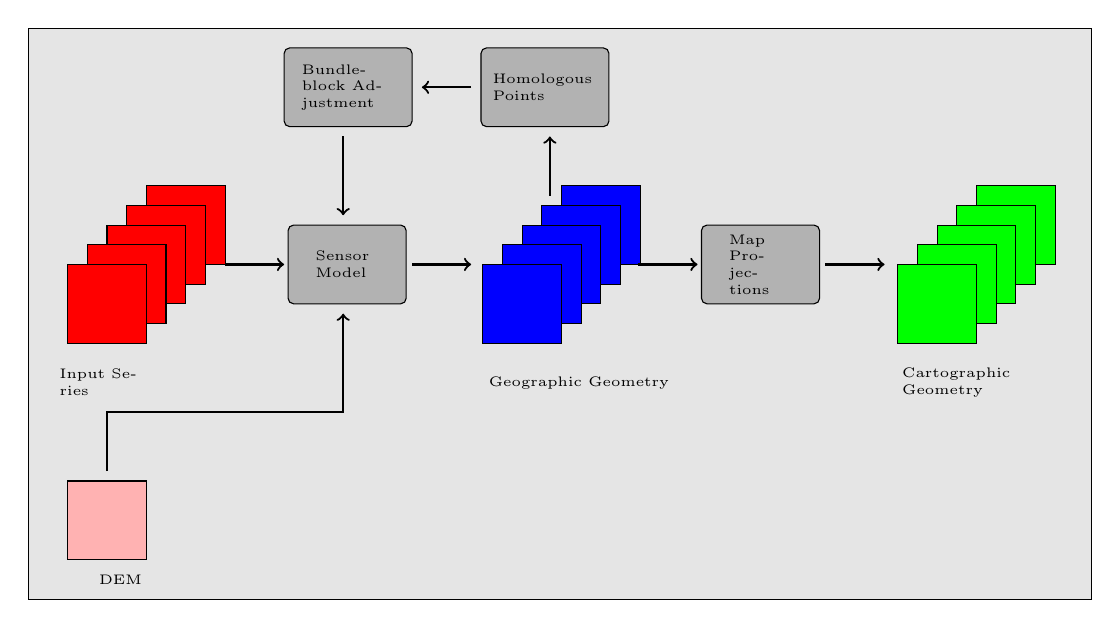
\begin{tikzpicture}[scale=0.25]
    \tiny
    \draw[fill=black!10] (-1,-12) rectangle (53,17);
     \foreach \x in {5,...,1}
       \draw[fill=red] (\x,\x) rectangle +(4,4);
     \node[fill=black!10, text width= 1.2cm] (InputSeries) at
       (3,-1) {Input Series};

     \draw[->,thick] (9,5) --  +(3,0);

     \draw[fill=black!30,rounded corners=2pt] (12.2,3) rectangle +(6,4);
     \node[text width= 0.7cm] (SensorModel) at (15,5) {Sensor Model};

     \draw[fill=red!30] (1,-10) rectangle +(4,4);
     \node[fill=black!10, text width= 1.2cm] (DEM) at
       (5,-11) {DEM};

     \draw[->,thick] (3,-5.5) --  ++(0,3) -- ++(12,0) -- ++(0,5);

     \draw[->,thick] (18.5,5) --  +(3,0);

     \foreach \x in {5,...,1}
       \draw[fill=blue,xshift=600pt] (\x,\x) rectangle +(4,4);
     \node[fill=black!10, text width= 2.8cm] (GeographicGeometry) at
       (28,-1) {Geographic Geometry};



       \draw[->,thick] (25.5,8.5) --  +(0,3);

     \draw[fill=black!30,rounded corners=2pt] (22,12) rectangle +(6.5,4);
     \node[text width= 0.7cm] (HomPoExtr) at (24,14) {Homologous
     Points};

     \draw[->,thick] (21.5,14) --  +(-2.5,0);

     \draw[fill=black!30,rounded corners=2pt] (12,12) rectangle +(6.5,4);
     \node[text width= 1.3cm] (BBAdj) at (15.5,14) {Bundle-block
     Adjustment};

     \draw[->,thick] (15,11.5) --  +(0,-4);


      \draw[->,thick] (30,5) --  +(3,0);

     \draw[fill=black!30,rounded corners=2pt] (33.2,3) rectangle +(6,4);
     \node[text width= 0.7cm] (MapProjection) at (36,5) {Map Projections};



     \draw[->,thick] (39.5,5) --  +(3,0);

     \foreach \x in {5,...,1}
       \draw[fill=green,xshift=1200pt] (\x,\x) rectangle +(4,4);
     \node[fill=black!10, text width= 1.8cm] (CartographicGeometry) at
       (47,-1) {Cartographic Geometry};

     %\draw[->,thick] (36,2) --  ++(0,-10) -- ++(-30,0);

  \end{tikzpicture}
  \itkcaption[Image Ortho-registration Procedure]{Image Ortho-registration Procedure.}
\label{fig:ImageOrtho-registrationProcedure}
\end{figure}

This chapter introduces the functionnalities available in OTB for
image ortho-registration. We define ortho-registration as the
procedure allowing to transform an image in sensor geometry to a
geographic or cartographic projection.\\

Figure \ref{fig:ImageOrtho-registrationProcedure} shows a synoptic
view of the different steps involved in a classical ortho-registration
processing chain able to deal with image series. These steps are the following:
\begin{itemize}
  \item Sensor modelling: the geometric sensor model allows to convert
  image coordinates (line, column) into geographic coordinates
  (latitude, longitude); a rigorous modelling needs a digital
  elevation model (DEM) in order to take into account the terrain
  topography.
  \item Bundle-block adjustment: in the case of image series, the
  geometric models and their parameters can be refined by using
  homologous points between the images. This is an optional step and
  not currently implemented in OTB.
  \item Map projection: this step allows to go from geographic
  coordinates to some specific cartographic projection as Lambert,
  Mercator or UTM.
\end{itemize}


\section{Sensor Models}
\ifitkFullVersion
\label{sec:SensorModels}
\fi

A sensor model is a set of equations giving the relationship between
image pixel $(l,c)$ coordinates and ground $(X,Y)$ coordinates for every
pixel in the image. Typically, the ground coordinates are given in a
geographic projection (latitude, longitude). The sensor model
can be expressed either from image to ground -- forward model -- or
from ground to image -- inverse model. This can be written as follows:

\begin{displaymath}
  \begin{array}{cc}
    Forward & \\
    X = f_x(l,c,h,\vec\theta) & Y = f_y(l,c,h,\vec\theta)\\
     & \\
    Inverse & \\
    l = g_l(X,Y,h,\vec\theta) & c = g_c(X,Y,h,\vec\theta)
  \end{array}
\end{displaymath}

Where $\vec\theta$ is the set of parameters which describe the sensor
and the acquisition geometry (platform altitude, viewing angle, focal
length for optical sensors, doppler centroid for SAR images, etc.).\\

In OTB, sensor models are implemented as \doxygen{itk}{Transform}s
(see section \ref{sec:Transforms} for details), which is the
appropriate way to express coordinate changes. The base class for
sensor models is \doxygen{otb}{SensorModelBase} from which the classes
\doxygen{otb}{InverseSensorModel} and
\doxygen{otb}{ForwardSensorModel} inherit.\\

As one may note from the model equations, the height of the ground, $h$,
must be known. Usually, it means that a Digital Elevation Model,
DEM, will be used.\\


\subsection{Types of Sensor Models}
\label{sec:TypesofSensorModels}
There exists two main types of sensor models. On one hand, we have the
so-called {\em physical models}, which are rigorous, complex,
eventually highly non-linear equations of the sensor geometry. As
such, they are difficult to inverse (obtain the inverse model from the
forward one and vice-versa). They have the significant advantage of having
parameters with physical meaning (angles, distances, etc.). They are
specific of each sensor, which means that a library of models is
required in the software. A library which has to be updated every time a new
sensor is available.\\

On the other hand, we have general analytical models, which
approximate the physical models. These models can take the form of
polynomials or ratios of polynomials, the so-called rational
polynomial functions or Rational Polynomial Coefficients, RPC, also
known as {\em Rapid Positioning Capability}.
Since they are approximations, they are less accurate than the
physical models. However, the achieved accuracy is usually high: in
the case of Pl\'eiades, RPC models have errors lower than 0.02 pixels
with respect to the physical model. Since these models have a standard
form they are easier to use and implement. However, they have the
drawback of having parameters (coefficients, actually) without
physical meaning.\\

OTB, through the use of the OSSIM library --
\url{http://www.ossim.org} -- offers models for most of current
sensors either through a physical or an analytical approach. This is
transparent for the user, since the geometrical model for a given
image is instantiated using the information stored in its meta-data. The 
search for a sensor model is not straightforward. It is done in several steps :
\begin{enumerate}
  \item Load an external \code{.geom} file specified through extended filenames
(if present)
  \item Load the \code{.geom} file attached with the input image (if present).
They share the same name, without extension.
  \item Search in the OSSIM plugin factory for a suitable model 
(\code{ossimplugins::ossimPluginProjectionFactory}). For instance, this
factory contains Pl\'eiades and TerraSar sensor models.
  \item If no model was found, search in the OSSIM projection factory 
(\code{ossimProjectionFactoryRegistry}). For instance this factory contains
Spot5, Landsat and Quickbird sensor models.
  \item If no model was found, search any RPC tags in the input image. When the
tags are present, an \code{ossimRpcModel} is created.
  \item If still no model was found, search for a valid sensor model in other
files attached to the current dataset. For instance, with a Sentinel 1 SAFE
dataset, it will inspect underlying \code{.tiff} files. With a VRT dataset, it
will inspect the files referenced by the VRT.
\end{enumerate}

Note that the \code{.geom} metadata file can store any sensor model recognized
by OSSIM.

\subsection{Using Sensor Models}
\label{sec:UsingSensorModels}

The transformation of an image in sensor geometry to geographic
geometry can be done using the following steps.
  \begin{enumerate}
    \item Read image meta-data and instantiate the model with the
    given parameters.
  \item Define the ROI in ground coordinates (this is your output
  pixel array)
  \item Iterate through the pixels of coordinates $(X,Y)$:
    \begin{enumerate}
      \item Get $h$ from the DEM
      \item Compute $(c,l) = G(X,Y,h,\vec\theta)$
      \item Interpolate pixel values if $(c,l)$ are not grid coordinates.
    \end{enumerate}
  \end{enumerate}

Actually, in OTB, you don't have to manually instantiate the sensor
model which is appropriate to your image. That is, you don't have to
manually choose a SPOT5 or a Quickbird sensor model. This task is
automatically performed by the \doxygen{otb}{ImageFileReader} class in
a similar way as the image format recognition is done. The appropriate
sensor model will then be included in the image meta-data, so you can
access it when needed.

\ifitkFullVersion
\input{SensorModelExample.tex}
\fi

\subsection{Evaluating Sensor Model}
\label{sec:EvaluatingSensorModels}

If no appropriate sensor model is available in the image meta-data,
OTB offers the possibility to estimate a sensor model from the image.

\input{EstimateRPCSensorModelExample.tex}


\subsection{Limits of the Approach}
\label{LimitsoftheApproach}

As you may understand by now, accurate geo-referencing needs accurate
DEM and also accurate sensor models and parameters. In the case where
we have several images acquired over the same area by different
sensors or different geometric configurations, geo-referencing (geographical coordinates) or ortho-rectification
(cartographic coordinates) is not usually enough. Indeed, when working
with image series we usually want to compare them (fusion, change
detection, etc.) at the pixel level.\\

Since common DEM and sensor parameters do not allow for such an
accuracy, we have to use clever strategies to improve the
co-registration of the images. The classical one consists in refining
the sensor parameters by taking homologous points between the images
to co-register. This is called bundle block adjustment and will be
implemented in coming versions of OTB.

Even if the model parameters are refined, errors due to DEM accuracy
can not be eliminated. In this case, image to image registration can
be applied. These approaches are presented in chapters
\ref{chap:ImageRegistration} and \ref{sec:DisparityMapEstimation}.

%% \section{Bundle-block adjustment}
%% Problem position
%%   \begin{itemize}
%%     \item The image series is geo-referenced (using the available DEM,
%%     and the prior sensor parameters).
%%     \item We assume that homologous points (GCPs, etc.) can be easily
%%     obtained from the geo-referenced series : $HP_i = (X_i,Y_i,h_i)$
%%     \item For each image, and each point, we can write:
%%     $(l_{ij},c_{ij}) = G_j(X_i,Y_i,h_i,\vec\theta_j)$
%%   \end{itemize}

%% \begin{tikzpicture}[scale=0.15]
%% \draw[fill=yellow!20] (-5.5,-15.5) rectangle (5.5,-5.5);
%%     \draw[step=0.5, gray, very thin] (-5.5,-15.5) grid (5.5,-5.5);

%%     \draw[fill=green!20,rotate=10] (-15.5,0.5) rectangle (-5.5,10.5);
%%     \draw[step=0.5, gray, very thin,rotate=10] (-15.5,0.5) grid>
%%     (-5.5,10.5);

%%     \draw[fill=blue!20,rotate=-10] (5.5,0.5) rectangle (15.5,10.5);
%%     \draw[step=0.5, gray, very thin,rotate=-10] (5.5,0.5) grid
%%     (15.5,10.5);


%%     \draw[fill=red!70] (1,-11) circle (0.2);

%%     \draw (1,-11) .. controls +(30:1cm) and +(60:1cm) .. (-10,7);

%%     \draw[fill=red!70] (-10,7) circle (0.2);

%%     \node (eq1) at (-12.2,-4) {$\scriptstyle{G_1(X_i,Y_i,h_i,\vec\theta_1)}$};

%%     \draw (1,-11) .. controls +(-30:1cm) and +(-60:1cm) .. (10,7);

%%     \draw[fill=red!70] (10,7) circle (0.2);

%%     \node (eq2) at (7.2,-3) {$\scriptstyle{G_2(X_i,Y_i,h_i,\vec\theta_2)}$};

%% \end{tikzpicture}
%% \begin{itemize}
%%       \item Everything is known.
%% \end{itemize}



%% Model refinement
%%   \begin{itemize}
%%     \item If we define $\vec\theta_j^R = \vec\theta_j +
%%     \vec{\Delta\theta_j}$ as the refined parameters,
%%     $\vec{\Delta\theta_j}$ are the unknowns of the model refinement
%%     problem.
%%     \item We have much more equations than unknowns if enough HPs are
%%     found.
%%     \item We solve using non-linear least squares estimation.
%%       \begin{itemize}
%% 	\item The derivatives of the sensor model with respect to its
%% 	parameters are needed.
%%       \end{itemize}
%%   \end{itemize}


%% Homologous point extraction
%% From manual to automatic procedures
%% \begin{itemize}
%%   \item Manual extraction can be used for a few images and for a few
%%   points
%%   \item We are interested in many images (long time series) and many
%%   points (in order to reduce registration errors)
%%   \item Proposed procedure
%%     \begin{enumerate}
%%       \item Choose candidate points
%%       \item Define a similarity measure
%%       \item Optimize the measure
%%     \end{enumerate}
%% \end{itemize}

%% Salient points
%% Similarity measures


\section{Map Projections}
\ifitkFullVersion
\label{sec:MapProjections}
\fi

Map projections describe the link between geographic coordinates and
cartographic ones. So map projections allow to represent a 2-dimensional manifold of a
3-dimensional space (the Earth surface) in a 2-dimensional space (a
map which used to be a sheet of paper!). This geometrical
transformation doesn't have a unique solution, so over the cartography
history, every country or region in the world has been able to express
the belief of being the center of the universe. In other words, every
cartographic projection tries to minimize the distortions of the 3D to
2D transformation for a given point of the Earth surface\footnote{We
  proposed to optimize an OTB map projection for Toulouse, but we
  didn't get any help from OTB users.}.

In OTB the \doxygen{otb}{MapProjection} class is derived from the
\doxygen{itk}{Transform} class, so the coordinate transformation
points are overloaded with map projection equations. The
\doxygen{otb}{MapProjection} class is templated over the type of
cartographic projection, which is provided by the OSSIM library. In
order to hide the complexity of the approach, some type definitions
for the more common projections are given in the file
\code{otbMapProjections.h} file.

Sometimes, you don't know at compile time what map projection you will need in
your application. In this case, the \doxygen{otb}{GenericMapProjection}
allow you to set the map projection at run-time by passing the WKT identification
for the projection.

\input{MapProjectionExample.tex}

You will seldom use a map projection by itself, but rather in an
ortho-rectification framework. An example is given in the next section.




\section{Orthorectification with OTB}
\ifitkFullVersion
\label{sec:OrthorectificationwithOTB}
\fi
\input{OrthoRectificationExample.tex}

\section{Vector data projection manipulation}
\ifitkFullVersion
\label{sec:VectorDataProjection}
\fi
\input{VectorDataProjectionExample.tex}

\section{Geometries projection manipulation}
\ifitkFullVersion
\label{sec:GeometriesProjection}
\fi
\input{GeometriesProjectionExample.tex}

\section{Elevation management with OTB}
\input{DEMHandlerExample.tex}

\section{Vector data area extraction}
\ifitkFullVersion
\label{sec:VectorDataAreaExtraction}
\fi
\input{VectorDataExtractROIExample.tex}

\input{Radiometry.tex}
\input{Fusion.tex}
\chapter{Feature Extraction}

% \section{Introduction}

Under the term {\em Feature Extraction} we include several techniques
aiming to detect or extract information of low level of abstraction
from images. These {\em features} can be objects : points, lines,
etc. They can also be measures : moments, textures, etc.

\section{Textures}
\subsection{Haralick Descriptors}

This example illustrates the use of the \doxygen{otb}{ScalarImageToTexturesFilter},
which compute the standard Haralick's textural features~\cite{Haralick1973} presented in table~\ref{tab:haralickStandardFeatures},
where $\mu_t$ and $\sigma_t$ are the mean and standard deviation of the row
(or column, due to symmetry) sums, $ \mu =  $ (weighted pixel average)
$ = \sum_{i,j}i \cdot g(i, j) =\sum_{i,j}j \cdot g(i, j) $ due to matrix summetry, and
$ \sigma =  $ (weighted pixel variance) $ = \sum_{i,j}(i - \mu)^2 \cdot g(i, j) =\sum_{i,j}(j - \mu)^2 \cdot g(i, j)  $
due to matrix symmetry.

\begin{table}
\begin{center}
\begin{tabular}{|c|c|}
\hline
& \\
Energy & $ f_1 = \sum_{i,j}g(i, j)^2 $ \\
& \\
\hline
& \\
Entropy & $ f_2 = -\sum_{i,j}g(i, j) \log_2 g(i, j)$, or 0 if $g(i, j) = 0$ \\
& \\
\hline
& \\
Correlation & $ f_3 = \sum_{i,j}\frac{(i - \mu)(j - \mu)g(i, j)}{\sigma^2} $ \\
& \\
\hline
& \\
Difference Moment &  $f_4 = \sum_{i,j}\frac{1}{1 + (i - j)^2}g(i, j) $ \\
& \\
\hline
& \\
Inertia (a.k.a. Contrast) & $ f_5 = \sum_{i,j}(i - j)^2g(i, j) $ \\
& \\
\hline
& \\
Cluster Shade & $ f_6 = \sum_{i,j}((i - \mu) + (j - \mu))^3 g(i, j) $ \\
& \\
\hline
Cluster Prominence & $ f_7 = \sum_{i,j}((i - \mu) + (j - \mu))^4 g(i, j) $ \\
& \\
\hline
& \\
Haralick's Correlation & $ f_8 = \frac{\sum_{i,j}(i, j) g(i, j) -\mu_t^2}{\sigma_t^2} $ \\
& \\
\hline
\end{tabular}
\itkcaption[Haralick features]{Haralick features~\cite{Haralick1973} available in \doxygen{otb}{ScalarImageToTexturesFilter}}
\end{center}
\label{tab:haralickStandardFeatures}
\end{table}

More features are available in \doxygen{otb}{ScalarImageToAdvancedTexturesFilter}.
\relatedClasses
\begin{itemize}
\item \doxygen{otb}{ScalarImageToAdvancedTexturesFilter}
\item \doxygen{otb}{ScalarImageToPanTexTextureFilter}
\item \doxygen{otb}{GreyLevelCooccurrenceIndexedList}
\end{itemize}

\input{TextureExample}

\subsection{PanTex}
\input{PanTexExample}

\subsection{Structural Feature Set}
\input{SFSExample}

\section{Interest Points}
\subsection{Harris detector}
\input{HarrisExample}
\subsection{SIFT detector}
\label{sec:SIFTDetector}
% \input{SIFTFastExample}
\InputIfFileExists{SIFTFastExample.tex}{}{}
\subsection{SURF detector}
\input{SURFExample}

\section{Alignments}
\label{sec:Alignments}
\input{AlignmentsExample}
\section{Lines}
\label{sec:LineDetectors}

\subsection{Line Detection}
\label{sec:LineDetection}
\input{RatioLineDetectorExample}
\input{CorrelationLineDetectorExample}
\input{AsymmetricFusionOfLineDetectorExample}
\input{ParallelLineDetectionExample}


\subsection{Segment Extraction}
\label{sec:SegmentExtraction}
\subsubsection{Local Hough Transform}
\input{LocalHoughExample}
%\input{ExtractSegmentsByStepsExample}
%\input{ExtractSegmentsExample}

\subsubsection{Line Segment Detector}
\label{sec:LSD}
\input{LineSegmentDetectorExample}
\subsection{Right Angle Detector}
\label{sec:RightAngleDetector}
\input{RightAngleDetectionExample}


\section{Density Features}
An interesting approach to feature extraction consists in computing
the density of previously detected features as simple edges or
interest points.
\subsection{Edge Density}
\input{EdgeDensityExample}
\subsection{SIFT Density}
\InputIfFileExists{SIFTDensityExample.tex}{}{}

% \input{SIFTDensityExample}

\section{Geometric Moments}

\subsection{Complex Moments}
\label{sec:ComplexMoments}
The complex geometric moments are defined as:
\begin {equation}
c_{pq} = \int\limits_{-\infty}^{+\infty}\int\limits_{-\infty}^{+\infty}(x + iy)^p(x- iy)^qf(x,y)dxdy,
\label{2.2}
\end{equation}
where $x$ and $y$ are the coordinates of the image $f(x,y)$, $i$ is the
imaginary unit and
$p+q$ is the order of $c_{pq}$. The geometric moments are
particularly useful in the case of scale changes.

\subsubsection{Complex Moments for Images}
\input{ComplexMomentsImageFunctionExample}
\subsubsection{Complex Moments for Paths}
\input{ComplexMomentPathExample}

\subsection{Hu Moments}
\label{sec:HuMoments}
Using the algebraic moment theory, H. Ming-Kuel obtained a family of 7
invariants with respect to planar transformations called Hu invariants,
\cite{hu}. Those invariants can be seen as nonlinear combinations of
the complex moments. Hu invariants have
been very much used in object recognition during the last 30 years,
since they are invariant to rotation, scaling and translation. \cite{flusserinv} gives their expressions :

\begin{equation}
\begin{array}{cccc}
\phi_1 = c_{11};& \phi_2 = c_{20}c_{02};& \phi_3 = c_{30}c_{03};& \phi_4 = c_{21}c_{12};\\
\phi_5 = Re(c_{30}c_{12}^3);& \phi_6 = Re(c_{21}c_{12}^2);& \phi_7 = Im(c_{30}c_{12}^3).&\\
\end{array}
\end{equation}


\cite{dudani} have used these invariants for the recognition of
aircraft silhouettes. Flusser and Suk have used them for image
registration, \cite{flusser_2}.

\subsubsection{Hu Moments for Images}
\input{HuMomentsImageFunctionExample}
%\subsubsection{Hu Moments for Paths}
%\input{HuMomentPathExample}


\subsection{Flusser Moments}
\label{sec:FlusserMoments}
The Hu invariants have been modified and
improved by several authors. Flusser used these moments in order to
produce a new family of descriptors of order higher than 3,
\cite{flusserinv}. These descriptors are invariant to scale and
rotation. They have the following expressions:
\begin {equation}
\begin{array}{ccc}
\psi_1  = c_{11} = \phi_1; &  \psi_2  = c_{21}c_{12} = \phi_4; & \psi_3  = Re(c_{20}c_{12}^2) = \phi_6;\\
\psi_4  = Im(c_{20}c_{12}^2); & \psi_5  = Re(c_{30}c_{12}^3) = \phi_5;
& \psi_6  = Im(c_{30}c_{12}^3) = \phi_7.\\
\psi_7  = c_{22}; & \psi_8  = Re(c_{31}c_{12}^2); & \psi_9  = Im(c_{31}c_{12}~2);\\
\psi_{10} = Re(c_{40}c_{12}^4); & \psi_{11} = Im(c_{40}c_{12}^2). &\\

\end{array}
\end {equation}

\textbf{Examples}
\subsubsection{Flusser Moments for Images}
\input{FlusserMomentsImageFunctionExample}
%\subsubsection{Flusser Moments for Paths}
%\input{FlusserMomentPathExample}

\section{Road extraction}
\label{sec:RoadExtraction}

Road extraction is a critical feature for an efficient use of high resolution satellite images. There are many applications of road extraction: update of GIS database, reference for image registration, help for identification algorithms and rapid mapping for example.  Road network can be used to register an optical image with a map or an optical image with a radar image for example. Road network extraction can help for other algorithms: isolated building detection, bridge detection. In these cases, a rough extraction can be sufficient. In the context of response to crisis, a fast mapping is necessary: within 6~hours, infrastructures for the designated area are required. Within this timeframe, a manual extraction is inconceivable and an automatic help is necessary.

\subsection{Road extraction filter}

\input{ExtractRoadExample}

\subsection{Step by step road extraction}

\input{ExtractRoadByStepsExample}


% \section{Seam carving}
% \label{sec:SeamCarving}
%
% \input{SeamCarvingExample}
%
% \input{SeamCarvingOtherExample}

\section{Cloud Detection}
\input{CloudDetectionExample}

\input{MultiScaleAnalysis.tex}
\input{ImageSegmentation.tex}
\input{ImageSimulation.tex}
\input{DimensionReduction.tex}
\chapter{Classification}

\section{Introduction}

Image classification consists in extracting added-value information from images. 
Such processing methods classify pixels within images into geographical connected 
zones with similar properties, and identified by a common class label. The 
classification can be either unsupervised or supervised.

Unsupervised classification does not require any additional information about the
properties of the input image to classify it. On the contrary, supervised methods 
need a preliminary learning to be computed over training datasets having similar 
properties than the image to classify, in order to build a classification model.

\section{Machine Learning Framework}

\subsection{Machine learning models}
\label{sec:MLGenericFramework}

The OTB classification is implemented as a generic Machine Learning
framework, supporting several possible machine learning libraries as backends.
The base class \doxygen{otb}{MachineLearningModel} defines this framework.
As of now libSVM (the machine learning library historically integrated in OTB),
machine learning methods of OpenCV library (\cite{opencv_library}) and also
Shark machine learning library (\cite{shark_library}) are available. Both
supervised and unsupervised classifiers are supported in the framework.

The current list of classifiers available through the same generic interface within the OTB is:

\begin{itemize}
  \item \textbf{LibSVM}: Support Vector Machines classifier based on libSVM.
  \item \textbf{SVM}: Support Vector Machines classifier based on OpenCV, itself based on libSVM.
  \item \textbf{Bayes}: Normal Bayes classifier based on OpenCV.
  \item \textbf{Boost}: Boost classifier based on OpenCV.
  \item \textbf{DT}: Decision Tree classifier based on OpenCV.
  \item \textbf{RF}: Random Forests classifier based on the Random Trees in OpenCV.
  \item \textbf{KNN}: K-Nearest Neighbors classifier based on OpenCV.
  \item \textbf{ANN}: Artificial Neural Network classifier based on OpenCV.
  \item \textbf{SharkRF} : Random Forests classifier based on Shark.
  \item \textbf{SharkKM} : KMeans unsupervised classifier based on Shark.
\end{itemize}

These models have a common interface, with the following major functions:
\begin{itemize}
  \item \code{SetInputListSample(InputListSampleType *in)} : set the list of input samples
  \item \code{SetTargetListSample(TargetListSampleType *in)} : set the list of target samples
  \item \code{Train()} : train the model based on input samples
  \item \code{Save(...)} : saves the model to file
  \item \code{Load(...)} : load a model from file
  \item \code{Predict(...)} : predict a target value for an input sample
  \item \code{PredictBatch(...)} : prediction on a list of input samples
\end{itemize}

The \code{PredictBatch(...)} function can be multi-threaded when
called either from a multi-threaded filter, or from a single location. In
the later case, it creates several threads using OpenMP.
There is a factory mechanism on top of the model class (see
\doxygen{otb}{MachineLearningModelFactory}). Given an input file,
the static function \code{CreateMachineLearningModel(...)} is able
to instantiate a model of the right type.

For unsupervised models, the target samples \textbf{still have to be set}. They
won't be used so you can fill a ListSample with zeros.

%-------------------------------------------------------------------------------
\subsection{Training a model}

The models are trained from a list of input samples, stored in a
\subdoxygen{itk}{Statistics}{ListSample}. For supervised classifiers, they
also need a list of targets associated to each input sample. Whatever the
source of samples, it has to be converted into a \code{ListSample} before
being fed into the model.

Then, model-specific parameters can be set. And finally, the \code{Train()}
method starts the learning step. Once the model is trained it can be saved
to file using the function \code{Save()}. The following examples show how
to do that.

\input{TrainMachineLearningModelFromSamplesExample.tex}

\input{TrainMachineLearningModelFromImagesExample.tex}

%-------------------------------------------------------------------------------
\subsection{Prediction of a model}

For the prediction step, the usual process is to:
\begin{itemize}
\item Load an existing model from a file.
\item Convert the data to predict into a \code{ListSample}.
\item Run the \code{PredictBatch(...)} function.
\end{itemize}

There is an image filter that perform this step on a whole image, supporting
streaming and multi-threading: \doxygen{otb}{ImageClassificationFilter}.

\ifitkFullVersion
\input{SupervisedImageClassificationExample.tex}
\fi

%-------------------------------------------------------------------------------
\subsection{Integration in applications}

The classifiers are integrated in several OTB Applications. There is a base
class that provides an easy access to all the classifiers:
\subdoxygen{otb}{Wrapper}{LearningApplicationBase}. As each machine learning
model has a specific set of parameters, the base class
\code{LearningApplicationBase} knows how to expose each type of classifier with
its dedicated parameters (a task that is a bit tedious so we want to implement
it only once). The \code{DoInit()} method creates a choice parameter named
\code{classifier} which contains the different supported classifiers along
with their parameters.

The function \code{Train(...)} provide an easy way to train the selected
classifier, with the corresponding parameters, and save the model to file.

On the other hand, the function \code{Classify(...)} allows to load a model
from file and apply it on a list of samples.

%%%%%%%%%%%%%%%%%%%%%%%%%%%%%%%%%%%%%%%%%%%%%%%%%%%%%%%%%%%%%%%%%%%%%%%%%%%%%%%%
\section{Supervised classification}

\subsection{Support Vector Machines}
\label{sec:SupportVectorMachines}

\subsubsection{SVM general description}
Kernel based learning methods in general and the Support Vector
Machines (SVM) in particular, have been introduced in the last years
in learning theory for classification and regression tasks,
\cite{vapnik}. SVM have been successfully applied to text
categorization, \cite{joachims}, and face recognition,
\cite{osuna}. Recently, they have been successfully used for the
classification of hyperspectral remote-sensing images, \cite{bruzzoneSVM}.

Simply stated, the approach consists in searching for the separating
surface between 2 classes by the determination of the subset of
training samples which best describes the boundary between the 2
classes. These samples are called support vectors and completely
define the classification system. In the case where the two classes are
nonlinearly separable, the method uses a kernel expansion in order to make
projections of the feature space onto higher dimensionality spaces
where the separation of the classes becomes linear.


\subsubsection{SVM mathematical formulation}

This subsection reminds the basic principles of SVM learning and
classification. A good tutorial on SVM can be found in, \cite{burges}.
 
We have $N$ samples represented by the couple $(y_i,\mathbf{x}_i),
i=1\ldots N$ where $y_i \in \{-1,+1\}$ is the class label and
$\mathbf{x}_i \in \mathbb{R}^n$ is the feature vector of dimension
$n$. A classifier is a function  $$f(\mathbf{x},\boldsymbol{\alpha}) :
\mathbf{x}\mapsto y$$ where $\boldsymbol{\alpha}$ are the classifier
parameters. The SVM finds the optimal separating hyperplane which
fulfills the following constraints :
    \begin{itemize}
      \item The samples with labels $+1$ and $-1$ are on different
      sides of the hyperplane.
      \item The distance of the closest vectors to the hyperplane is
      maximised. These are the support vectors (SV) and this distance is
      called the margin.
    \end{itemize}

    The separating hyperplane has the equation
    $$\mathbf{w}\cdot\mathbf{x}+b=0;$$ with $\mathbf{w}$ being its
    normal vector and $x$ being any point of the hyperplane. The
    orthogonal distance to the origin is given by
    $\frac{|b|}{\|\mathbf{w}\|}$. Vectors located outside the
    hyperplane have either $\mathbf{w}\cdot\mathbf{x}+b>0$ or
      $\mathbf{w}\cdot\mathbf{x}+b<0$.

    Therefore, the classifier function can be written as
    $$f(\mathbf{x},\mathbf{w}, b)=sgn(\mathbf{w}\cdot\mathbf{x}+b).$$
    
The SVs are placed on two hyperplanes which are parallel to the
      optimal separating one. In order to find the optimal
      hyperplane, one sets $\mathbf{w}$ and
      $b$ : $$\mathbf{w}\cdot\mathbf{x}+b=\pm 1.$$

Since there must not be any vector inside the margin, the following
constraint can be used:
    $$\mathbf{w}\cdot\mathbf{x}_i+b\ge +1\text{ if }y_i=+1;$$
    $$\mathbf{w}\cdot\mathbf{x}_i+b\le -1\text{ if }y_i=-1;$$ which
    can be rewritten as $$y_i(\mathbf{w}\cdot\mathbf{x}_i+b)-1\ge 0~  ~ \forall i.$$

    The orthogonal distances of the 2 parallel hyperplanes to the
    origin are $\frac{|1-b|}{\|\mathbf{w}\|}$ and
      $\frac{|-1-b|}{\|\mathbf{w}\|}$. Therefore the modulus of the
    margin is equal to $\frac{2}{\|\mathbf{w}\|}$ and it has to be
    maximised.

    Thus, the problem to be solved is:

	\begin{itemize}
	\item Find $\mathbf{w}$ and $b$ which minimise
	 $\left\{ \frac{1}{2}\|\mathbf{w}\|^2 \right\}$
	\item under the constraint :
	 $y_i(\mathbf{w}\cdot\mathbf{x}_i+b)\ge 1~  ~ i=1\ldots N.$
	\end{itemize}

	This problem can be solved by using the Lagrange multipliers
	with one multiplier per sample. It can be shown that only the
	support vectors will have a positive Lagrange multiplier.

	In the case where the two classes are not exactly linearly
	separable, one can modify the constraints above by using 
      $$\mathbf{w}\cdot\mathbf{x}_i+b\ge +1 - \xi_i \text{ if }y_i=+1;$$
    $$\mathbf{w}\cdot\mathbf{x}_i+b\le -1+\xi_i \text{ if }y_i=-1;$$
    $$\xi_i\ge 0~  ~\forall i.$$

	If $\xi_i > 1$, one considers that the sample is wrong. The
	function which has then to be minimised is
	$\frac{1}{2}\|\mathbf{w}\|^2 + C\left( \sum_i \xi_i\right); $,
	where $C$ is a tolerance parameter. The optimisation problem
	is the same than in the linear case, but one multiplier has to
	be added for each new constraint $\xi_i\ge 0$.

	If the decision surface needs to be non-linear, this solution
	cannot be applied and the kernel approach has to be adopted.


One drawback of the SVM is that, in their basic version, they can only
solve two-class problems. Some works exist in the field of multi-class
SVM (see \cite{allwein00reducing,weston98multiclass}, and the
comparison made by \cite{hsu01comparison}), but they are
not used in our system.

You have to be aware that to achieve better convergence of the algorithm it is 
strongly advised to normalize feature vector components in the $[-1;1]$ 
interval.

For problems with $N > 2$ classes, one can choose either to train $N$
SVM (one class against all the others), or to train $N\times(N-1)$ SVM
(one class against each of the others). In the second approach, which
is the one that we use, the final decision is taken by choosing the
class which is most often selected by the whole set of SVM.


%-------------------------------------------------------------------------------
\subsection{Shark Random Forests}

The Random Forests algorithm is also available in OTB machine learning
framework. This model builds a set of decision trees. Each tree may not give
a reliable prediction, but taking them together, they form a robust classifier.
The prediction of this model is the mode of the predictions of individual trees.

There are two implementations: one in OpenCV and the other on in
Shark. The Shark implementation has a noteworthy advantage: the training step
is parallel. It uses the following parameters:
\begin{itemize}
\item The number of trees to train
\item The number of random attributes to investigate at each node
\item The maximum node size to decide a split
\item The ratio of the original training dataset to use as the out of bag sample
\end{itemize}

Except these specific parameter, its usage is exactly the same as the other
machine learning models (such as the SVM model).

%-------------------------------------------------------------------------------
\subsection{Generic Kernel SVM (deprecated)}
OTB has developed a specific interface for user-defined kernels. However, the 
following functions use a deprecated OTB interface. The code source for these
Generic Kernels has been removed from the official repository. It is now
available as a remote module: \href{https://github.com/jmichel-otb/GKSVM}{GKSVM}.

A function $k(\cdot,\cdot)$ is considered to be a kernel when:
\begin{align}\label{eqMercer}
        \forall g(\cdot) \in {\cal L}^2(\mathbbm{R}^n) \quad & \text{so 
that} \quad
        \int g(\boldsymbol{x})^2 d\boldsymbol{x} \text{ be finite,} \\
        & \text{then} \quad \int k(\boldsymbol{x},\boldsymbol{y}) \, 
g(\boldsymbol{x})
        \, g(\boldsymbol{y}) \, d\boldsymbol{x} d\boldsymbol{y} \geqslant 0,
        \notag
\end{align}
which is known as the {\em Mercer condition\/}.

When defined through the OTB, a kernel is a class that inherits from
\code{GenericKernelFunctorBase}. Several virtual functions have to 
be overloaded:
\begin{itemize}
\item The \code{Evaluate} function, which implements the behavior of the 
kernel
itself. For instance, the classical linear kernel could be re-implemented
with:
\begin{verbatim}
        double
        MyOwnNewKernel
        ::Evaluate ( const svm_node * x, const svm_node * y,
                     const svm_parameter & param ) const
        {
                return this->dot(x,y);
        }
\end{verbatim}
This simple example shows that the classical dot product is already 
implemented
into \code{otb::GenericKernelFunctorBase::dot()} as a protected
function.
\item The \code{Update()} function which synchronizes local variables and 
their
integration into the initial SVM procedure. The following examples will show
the way to use it.
\end{itemize}

Some pre-defined generic kernels have already been implemented in OTB:
\begin{itemize}
\item \code{otb::MixturePolyRBFKernelFunctor} which implements a 
linear mixture
of a polynomial and a RBF kernel;
\item \code{otb::NonGaussianRBFKernelFunctor} which implements a non
gaussian RBF kernel;
\item \code{otb::SpectralAngleKernelFunctor}, a kernel that integrates
the Spectral Angle, instead of the Euclidean distance, into an inverse 
multiquadric kernel.
This kernel may be appropriated when using multispectral data.
\item \code{otb::ChangeProfileKernelFunctor}, a kernel which is
dedicated to the supervized classification of the multiscale change profile
presented in section \ref{sec:KullbackLeiblerProfile}.
\end{itemize}

\subsubsection{Learning with User Defined Kernels}
\label{sec:Learningwithuserdefinedkernel}
\ifitkFullVersion
\input{SVMGenericKernelImageModelEstimatorExample.tex}
\fi

\subsubsection{Classification with user defined kernel}

\ifitkFullVersion
\input{SVMGenericKernelImageClassificationExample.tex}
\fi


%%%%%%%%%%%%%%%%%%%%%%%%%%%%%%%%%%%%%%%%%%%%%%%%%%%%%%%%%%%%%%%%%%%%%%%%%%%%%%%%
\section{Unsupervised classification}

\subsection{K-Means Classification}
\label{sec:KMeansClassifier}

\subsubsection{Shark version}

The KMeans algorithm has been implemented in Shark library, and has been
wrapped in the OTB machine learning framework. It is the first unsupervised
algorithm in this framework. It can be used in the same way as other machine
learning models. Remember that even if unsupervised model don't use a label
information on the samples, the target ListSample still has to be set in
\code{MachineLearningModel}. A ListSample filled with zeros can be used.

This model uses a hard clustering model with the following parameters:
\begin{itemize}
\item The maximum number of iterations
\item The number of centroids (K)
\item An option to normalize input samples
\end{itemize}

As with Shark Random Forests, the training step is parallel.

\subsubsection{Simple version}
\ifitkFullVersion
\input{ScalarImageKmeansClassifier.tex}
\fi
\ifitkFullVersion
\input{ScalarImageKmeansModelEstimator.tex}
\fi

\subsubsection{General approach}
\ifitkFullVersion
\input{KMeansImageClassificationExample.tex}
\fi

\subsubsection{k-d Tree Based k-Means Clustering}
\label{sec:KdTreeBasedKMeansClustering}
\ifitkFullVersion
\input{KdTreeBasedKMeansClustering.tex}
\fi
%-------------------------------------------------------------------------------
\subsection{Kohonen's Self Organizing Map}
\label{sec:SOM}
\input{Kohonen}
%%%1. Construction SOM
\subsubsection{Building a color table}
\label{sec:SOMColorTable}
\input{SOMExample}
\subsubsection{SOM Classification}
\label{sec:SOMClassification}
\input{SOMClassifierExample}

\subsubsection{Multi-band, streamed classification}

\ifitkFullVersion
\input{SOMImageClassificationExample.tex}
\fi

%%%2. Lecture SOM et ensemble de vecteurs autre image pour construire
%%%ActivationMAP 

%\subsection{Bayesian classification}
%-------------------------------------------------------------------------------
\subsection{Bayesian Plug-In Classifier}
\label{sec:BayesianPluginClassifier}

\ifitkFullVersion
\input{BayesianPluginClassifier.tex}
\fi

%-------------------------------------------------------------------------------
\subsection{Expectation Maximization Mixture Model Estimation}
\label{sec:ExpectationMaximizationMixtureModelEstimation}

\ifitkFullVersion
\input{ExpectationMaximizationMixtureModelEstimator.tex}
\fi




%-------------------------------------------------------------------------------
\subsection{Statistical Segmentations}
\label{sec:StatisticalSegmentations}

%\subsection{Markov Random Fields}

\subsubsection{Stochastic Expectation Maximization}
\label{sec:SEM}

The Stochastic Expectation Maximization (SEM) approach is a stochastic 
version of the EM mixture estimation seen on
section~\ref{sec:ExpectationMaximizationMixtureModelEstimation}. It has been 
introduced by \cite{CeDi95} to prevent convergence of the EM approach from
local minima. It avoids the analytical maximization issued by integrating a
stochastic sampling procedure in the estimation process. It induces an almost
sure (a.s.) convergence to the algorithm.

From the initial two step formulation of the EM mixture estimation, the SEM
may be decomposed into 3 steps:
\begin{enumerate}
\item \textbf{E-step}, calculates the expected membership values for each 
measurement vector to each classes.
\item \textbf{S-step}, performs a stochastic sampling of the membership vector
to each classes, according to the membership values computed in the E-step.
\item \textbf{M-step}, updates the parameters of the membership probabilities
(parameters to be defined through the class
\subdoxygen{itk}{Statistics}{ModelComponentBase} and its inherited classes).
\end{enumerate}
The implementation of the SEM has been turned to a contextual SEM in the sense
where the evaluation of the membership parameters is conditioned to
membership values of the spatial neighborhood of each pixels.

\ifitkFullVersion
\input{SEMModelEstimatorExample.tex}
\fi

%-------------------------------------------------------------------------------
\subsection{Classification using Markov Random Fields}
\label{sec:MarkovRandomField}

Markov Random Fields are probabilistic models that use the statistical
dependency between
pixels in a neighborhood to infeer the value of a give pixel.

\subsubsection{ITK framework}
\label{sec:MarkovRandomFieldITK}
The
\subdoxygen{itk}{Statistics}{MRFImageFilter} uses the maximum a posteriori (MAP)
estimates for modeling the MRF. The object traverses the data set and uses the
model generated by the Mahalanobis distance classifier to get the the distance
between each pixel in the data set to a set of known classes, updates the
distances by evaluating the influence of its neighboring pixels (based on a MRF
model) and finally, classifies each pixel to the class which has the minimum
distance to that pixel (taking the neighborhood influence under consideration).
The energy function minimization is done using the iterated conditional modes
(ICM) algorithm \cite{Besag1986}.

\ifitkFullVersion
\input{ScalarImageMarkovRandomField1.tex}
\fi

\subsubsection{OTB framework}
\label{sec:MarkovRandomFieldOTB}
The ITK approach was considered not to be flexible enough for some
remote sensing applications. Therefore, we decided to implement our
own framework.
\index{Markov}

\begin{figure}[th]
  \centering
  \includegraphics[width=0.7\textwidth]{MarkovFramework.eps}
  \itkcaption[OTB Markov Framework]{OTB Markov Framework.}
  \label{fig:markovFramework}
\end{figure}

\index{Markov!Classification}
\ifitkFullVersion
\input{MarkovClassification1Example.tex}
\fi

\index{Markov!Classification}
\ifitkFullVersion
\input{MarkovClassification2Example.tex}
\fi

\index{Markov!Classification}
\ifitkFullVersion
\input{MarkovClassification3Example.tex}
\fi

\index{Markov!Regularization}
\ifitkFullVersion
\input{MarkovRegularizationExample.tex}
\fi

%%%%%%%%%%%%%%%%%%%%%%%%%%%%%%%%%%%%%%%%%%%%%%%%%%%%%%%%%%%%%%%%%%%%%%%%%%%%%%%%
\section{Fusion of Classification maps}

\subsection{General approach of image fusion}
In order to obtain a relevant image classification it is sometimes necessary to 
fuse several classification maps coming from different classification methods 
(SVM, KNN, Random Forest, Artificial Neural Networks,...). The fusion of 
classification maps combines them in a more robust and precise one. Two methods are 
available in the OTB: the majority voting and the Demspter Shafer framework.

%-------------------------------------------------------------------------------
\subsection{Majority voting}
\subsubsection{General description}
For each input pixel, the Majority Voting method consists in choosing the more 
frequent class label among all classification maps to fuse. In case of not unique 
more frequent class labels, the undecided value is set for such pixels in 
the fused output image.

\subsubsection{An example of majority voting fusion}
\ifitkFullVersion
\input{MajorityVotingFusionOfClassificationMapsExample.tex}
\fi

%-------------------------------------------------------------------------------
\subsection{Dempster Shafer}

\subsubsection{General description}
A more adaptive fusion method using the Dempster Shafer theory 
(\href{http://en.wikipedia.org/wiki/Dempster-Shafer_theory}{http://en.wikipedia.org/wiki/Dempster-Shafer\_theory}) 
is available within the OTB. This method is adaptive as it is based on the 
so-called belief function of each class label for each classification map. Thus, 
each classified pixel is associated to a degree of confidence according to the 
classifier used. In the Dempster Shafer framework, the expert's point of view 
(i.e. with a high belief function) is considered as the truth. In order to 
estimate the belief function of each class label, we use the Dempster Shafer 
combination of masses of belief for each class label and for each classification 
map. In this framework, the output fused label of each pixel is the one with the 
maximal belief function.

Like for the majority voting method, the Dempster Shafer fusion handles not 
unique class labels with the maximal belief function. In this case, the output 
fused pixels are set to the undecided value.

The confidence levels of all the class labels are estimated from a comparison of 
the classification maps to fuse with a ground truth, which results in a 
confusion matrix. For each classification maps, these confusion matrices are then 
used to estimate the mass of belief of each class label.


\subsubsection{Mathematical formulation of the combination algorithm}

A description of the mathematical formulation of the Dempster Shafer combination 
algorithm is available in the following OTB Wiki page: 
\href{http://wiki.orfeo-toolbox.org/index.php/Information_fusion_framework}{http://wiki.orfeo-toolbox.org/index.php/Information\_fusion\_framework}.

\subsubsection{An example of Dempster Shafer fusion}
\ifitkFullVersion
\input{DempsterShaferFusionOfClassificationMapsExample.tex}
\fi


%%%%%%%%%%%%%%%%%%%%%%%%%%%%%%%%%%%%%%%%%%%%%%%%%%%%%%%%%%%%%%%%%%%%%%%%%%%%%%%%
\section{Classification map regularization}

%\subsection{Regularization by neighborhood-based majority voting}

\ifitkFullVersion
\input{ClassificationMapRegularizationExample.tex}
\fi





\chapter{Object-based Image Analysis }\label{sec:OBIA}

\section{Object Filtering based on radiometric and statistics attributes}
\input{RadiometricAttributesLabelMapFilterExample.tex}

\section{Hoover metrics to compare segmentations}
\input{HooverMetricsEstimation.tex}

%\section{Objects vectorization}
%\input{LabelMapVectorization.tex}

%\section{Object-based classification}

\chapter{Change Detection}

\section{Simple Detectors}
\label{sec:SimpleDetectors}
\subsection{Mean Difference}
\label{sec:MeanDifference}

The simplest change detector is based on the pixel-wise differencing
of image values: 
\begin{equation}
I_{D}(i,j)=I_{2}(i,j)-I_{1}(i,j).
\end{equation}

In order to make the algorithm robust to noise, one actually uses
local means instead of pixel values.

\input{DiffChDet}

\subsection{Ratio Of Means}
\label{sec:RatioOfMeans}

This detector is similar to the previous one except that it uses a
ratio instead of the difference:
\begin{equation}
\displaystyle I_{R}(i,j) = \frac{\displaystyle I_{2}(i,j)}{\displaystyle I_{1}(i,j)}.
\end{equation}

The use of the ratio makes this detector robust to multiplicative
noise which is a good model for the speckle phenomenon which is
present in radar images.

In order to have a bounded and normalized detector the following
expression is actually used:


\begin{equation}
\displaystyle I_{R}(i,j) = 1 - min \left(\frac{\displaystyle I_{2}(i,j)}{\displaystyle I_{1}(i,j)},\frac{\displaystyle I_{1}(i,j)}{\displaystyle I_{2}(i,j)}\right).
\end{equation}


\input{RatioChDet}


\section{Statistical Detectors}
\label{sec:StatisticalDetectors}

\subsection{Distance between local distributions}
\label{sec:KullbackLeiblerDistance}

This detector is similar to the ratio of means detector (seen in the 
previous section page~\pageref{sec:RatioOfMeans}). Nevertheless, 
instead of the comparison of means, the comparison is performed to
the complete distribution of the two Random Variables (RVs)~\cite{Inglada03}.

The detector is based on the Kullback-Leibler distance between probability 
density functions (pdfs). In the neighborhood of each pixel of the pair 
of images $I_1$ and $I_2$ to be compared, the distance between local pdfs 
$f_1$ and $f_2$ of RVs $X_1$ and $X_2$ is evaluated by:
\begin{align}
  {\cal K}(X_1,X_2) &= K(X_1|X_2) + K(X_2|X_1) \\
  \text{with} \qquad
  K(X_j | X_i) &= \int_{\mathbbm{R}} 
      \log \frac{f_{X_i}(x)}{f_{X_j}(x)} f_{X_i}(x) dx,\qquad i,j=1,2.
\end{align}
In order to reduce the computational time, the local pdfs $f_1$ and $f_2$ 
are not estimated through histogram computations but rather by a cumulant
expansion, namely the Edgeworth expansion, with is based on the 
cumulants of the RVs:
\begin{equation}\label{eqEdgeworthExpansion}
f_X(x) = \left( 1 + \frac{\kappa_{X;3}}{6} H_3(x) 
					+ \frac{\kappa_{X;4}}{24} H_4(x)
					+ \frac{\kappa_{X;5}}{120} H_5(x)
					+ \frac{\kappa_{X;6}+10 \kappa_{X;3}^2}{720} H_6(x) \right) {\cal G}_X(x).
\end{equation}
In eq.~\eqref{eqEdgeworthExpansion}, ${\cal G}_X$ stands for the Gaussian pdf
which has the same mean and variance as the RV $X$. The $\kappa_{X;k}$
coefficients are the cumulants of order $k$, and $H_k(x)$ are the 
Chebyshev-Hermite polynomials of order $k$ (see~\cite{Inglada07} for deeper
explanations).

\input{KullbackLeiblerDistanceChDet}

\subsection{Local Correlation}
\label{sec:LocalCorrelation}
The correlation coefficient measures the likelihood of a linear
relationship between two random variables:
\begin{equation}
\begin{split}
I_\rho(i,j) &= \frac{1}{N}\frac{\sum_{i,j}(I_1(i,j)-m_{I_1})(I_2(i,j)-m_{I_2})}{\sigma_{I_1}
\sigma_{I_2}}\\
& = \sum_{(I_1(i,j),I_2(i,j))}\frac{(I_1(i,j)-m_{I_1})(I_2(i,j)-m_{I_2})}{\sigma_{I_1}
\sigma_{I_2}}p_{ij}
\end{split}
\end{equation}

where $I_1(i,j)$ and $I_2(i,j)$ are the pixel values of the 2 images and
$p_{ij}$ is the joint probability density. This is like using a linear model:
\begin{equation}
I_2(i,j) = (I_1(i,j)-m_{I_1})\frac{\sigma_{I_2}}{\sigma_{I_1}}+m_{I_2}
\end{equation}
for which we evaluate the likelihood with  $p_{ij}$.

With respect to the difference detector, this one will be robust to
illumination changes.
\input{CorrelChDet.tex}

\section{Multi-Scale Detectors}
\label{sec:MultiScaleDetectors}

\subsection{Kullback-Leibler Distance between distributions}
\label{sec:KullbackLeiblerProfile}

This technique is an extension of the distance between distributions 
change detector presented in section~\ref{sec:KullbackLeiblerDistance}.
Since this kind of detector is based on cumulants estimations through
a sliding window, the idea is just to upgrade the estimation of the cumulants
by considering new samples as soon as the sliding window is increasing in size.

Let's consider the following problem: how to update the moments when a
$N+1^{th}$ observation $x_{N+1}$ is added to a set of observations $\{x_1, x_2, \ldots,
x_N\}$ already considered.
The evolution of the central moments may be characterized by:
\begin{align}\label{eqMomentN}
	\mu_{1,[N]} & = \frac{1}{N} s_{1,[N]} \\
	\mu_{r,[N]} & = \frac{1}{N} \sum_{\ell = 0}^r \binom{r}{\ell} 
									\left( -\mu_{1,[N]} \right)^{r-\ell}
									s_{\ell,[N]}, \notag
\end{align}
where the
notation $s_{r,[N]} = \sum_{i=1}^N x_i^r$ has been used.
Then, Edgeworth series is updated also by transforming moments to
cumulants by using:
\begin{equation}\label{eqCumsMoms}
  \begin{split}
\kappa_{X;1} &= \mu_{X;1}\\
\kappa_{X;2} &= \mu_{X;2}-\mu_{X;1}^2\\
\kappa_{X;3} &= \mu_{X;3} - 3\mu_{X;2} \mu_{X;1} + 2\mu_{X;1}^3\\
\kappa_{X;4} &= \mu_{X;4} - 4\mu_{X;3} \mu_{X;1} - 3\mu_{X;2}^2 + 12 \mu_{X;2} \mu_{X;1}^2 - 6\mu_{X;1}^4.
  \end{split}
\end{equation}
It yields a set of images that represent the change measure according to an
increasing size of the analysis window.

\input{KullbackLeiblerProfileChDet}

\section{Multi-components detectors}

\subsection{Multivariate Alteration Detector}

\input{MultivariateAlterationDetector}




\chapter{Hyperspectral}

\input{HyperspectralUnmixingExample}


\input{Visualization.tex}

%%% \input{Applications.tex}



\part{Developer's guide}\label{part:developerguide}
\chapter{Iterators}
\label{sec:ImageIteratorsChapter}
\index{Iterators!image|(}
\index{Generic Programming}
This chapter introduces the \emph{image iterator}, an important generic
programming construct for image processing in ITK.  An iterator is a
generalization of the familiar C programming language pointer used to
reference data in memory.  ITK has a wide variety of image iterators, some of
which are highly specialized to simplify common image processing tasks.

The next section is a brief introduction that defines iterators in the context
of ITK.  Section \ref{sec:IteratorsInterface} describes the programming
interface common to most ITK image iterators.
Sections~\ref{sec:ImageIterators}--\ref{sec:NeighborhoodIterators} document
specific ITK iterator types and provide examples of how they are used.

\section{Introduction}
\label{sec:IteratorsIntroduction}
% Further define iterators in the context of generic programming.
\index{generic programming}
\index{Iterators!definition of}
Generic programming models define functionally independent components called
\emph{containers} and \emph{algorithms}.  Container objects store data and
algorithms operate on data.  To access data in containers, algorithms use a
third class of objects called \emph{iterators}.  An iterator is an
abstraction of a memory pointer.  Every container type must define its own
iterator type, but all iterators are written to provide a common interface so
that algorithm code can reference data in a generic way and maintain
functional independence from containers.

The iterator is so named because it is used for \emph{iterative}, sequential
access of container values.  Iterators appear in \code{for} and
\code{while} loop constructs, visiting each data point in turn.  
A C pointer, for example, is a type of iterator.  It can be moved
forward (incremented) and backward (decremented) through memory to
sequentially reference elements of an array. Many iterator implementations
have an interface similar to a C pointer.

\index{Iterators!advantages of}
In ITK we use iterators to write generic image processing code for images
instantiated with different combinations of pixel type, pixel
container type, and dimensionality.  Because ITK image iterators are
specifically designed to work with \emph{image} containers, their interface and
implementation is optimized for image processing tasks.  Using the ITK
iterators instead of accessing data directly through the
\doxygen{otb}{Image} interface has many advantages. Code is more
compact and often generalizes automatically to higher dimensions, algorithms
run much faster, and iterators simplify tasks such as multithreading and
neighborhood-based image processing.


\section{Programming Interface}
\label{sec:IteratorsInterface}

\index{Iterators!programming interface|(}
%Creating iterators
This section describes the standard ITK image iterator programming interface.
Some specialized image iterators may deviate from this standard or provide
additional methods.

\subsection{Creating Iterators}
\label{sec:CreatingIterators}

\index{Iterators!construction of}
All image iterators have at least one template parameter that is the image
type over which they iterate.  There is no restriction on the dimensionality
of the image or on the pixel type of the image.

\index{Iterators!and image regions}

An iterator constructor requires at least two arguments, a smart pointer to the
image to iterate across, and an image region. The image region, called the
\emph{iteration region}, is a rectilinear area in which iteration is
constrained.  The iteration region must be wholly contained within the image.
More specifically, a valid iteration region is any subregion of the image
within the current \code{BufferedRegion}.  See Section~\ref{sec:ImageSection}
for more information on image regions.

\index{Iterators!const}
There is a const and a non-const version of most ITK image iterators. A
non-const iterator cannot be instantiated on a non-const image pointer.
Const versions of iterators may read, but may not write pixel values.

Here is a simple example that defines and constructs a simple image iterator
for an \doxygen{otb}{Image}.

\small
\begin{verbatim}
  typedef otb::Image<float, 3> ImageType;
  typedef itk::ImageRegionConstIterator< ImageType > ConstIteratorType;
  typedef itk::ImageRegionIterator< ImageType > IteratorType;

  ImageType::Pointer image = SomeFilter->GetOutput();

  ConstIteratorType constIterator( image, image->GetRequestedRegion() );
  IteratorType iterator( image, image->GetRequestedRegion() );
\end{verbatim}
\normalsize

\subsection{Moving Iterators}
\label{sec:MovingIterators}
An iterator is described as \emph{walking} its iteration region.  At any
time, the iterator will reference, or ``point to'', one pixel location in the
N-dimensional (ND) image.  \emph{Forward iteration} goes from the beginning
of the iteration region to the end of the iteration region.  \emph{Reverse
iteration}, goes from just past the end of the region back to the beginning.
There are two corresponding starting positions for iterators, the
\emph{begin} position and the \emph{end} position.  An iterator can be moved
directly to either of these two positions using the following methods.

\index{forward iteration}
\index{reverse iteration}
\index{iteration region}
\index{Iterators!GoToBegin()}

\begin{itemize}
\item \textbf{\code{GoToBegin()}} Points the iterator to the first valid
data element in the region.

\index{Iterators!GoToEnd()}
\item \textbf{\code{GoToEnd()}} Points the iterator to \emph{one position past}
the last valid element in the region.
\end{itemize}

Note that the end position is not actually located within the iteration region.  This is
important to remember because attempting to dereference an iterator at its end
position will have undefined results.

%Moving iteators
ITK iterators are moved back and forth across their iterations using the 
decrement and increment operators.

\index{Iterators!operator++()}
\begin{itemize}
\item \textbf{\code{operator++()}} Increments the iterator one position in the
positive direction.  Only the prefix increment operator is defined for ITK image
iterators.

\index{Iterators!operator--}
\item \textbf{\code{operator--()}} Decrements the iterator one position in the
negative direction.  Only the prefix decrement operator is defined for ITK
image iterators. 
\end{itemize}

Figure~\ref{fig:WalkingIterator} illustrates typical iteration over
an image region.  Most iterators increment and decrement in the direction of
the fastest increasing image dimension, wrapping to the first position in the
next higher dimension at region boundaries.  In other words, an
iterator first moves across columns, then down rows, then from slice to slice,
and so on.

\begin{figure}
\centering
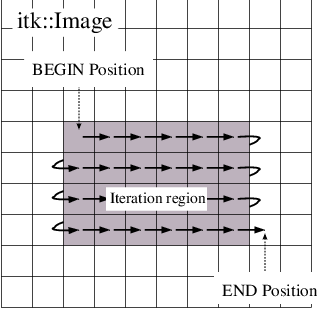
\includegraphics[width=0.4\textwidth]{IteratorFigure1.eps}
\itkcaption[ITK image iteration]{Normal path of an iterator through a 
2D image.  The iteration region is shown in a darker shade.  An arrow denotes
a single iterator step, the result of one \code{++} operation.}
\protect\label{fig:WalkingIterator}
\end{figure}

In addition to sequential iteration through the image, some iterators may define
random access operators.  Unlike the increment operators, random access
operators may not be optimized for speed and require some knowledge of the
dimensionality of the image and the extent of the iteration region to use properly.

\begin{itemize}
\index{Iterators!operator+=()}
\item \textbf{\code{operator+=( OffsetType )}} Moves the iterator to the pixel
position at the current index plus specified \doxygen{itk}{Offset}.

\index{Iterators!operator-=()}
\item \textbf{\code{operator-=( OffsetType )}} Moves the iterator to 
the pixel position at the current index minus specified Offset.

\index{Iterators!SetPosition()}
\item \textbf{\code{SetPosition( IndexType )}} Moves the iterator to the given
\doxygen{itk}{Index} position.
\end{itemize}

The \code{SetPosition()} method may be extremely slow for more complicated
iterator types. In general, it should only be used for setting a starting
iteration position, like you would use \code{GoToBegin()} or \code{GoToEnd()}.

Some iterators do not follow a predictable path through their
iteration regions and have no fixed beginning or ending pixel
locations.  A conditional iterator, for example, visits pixels only if
they have certain values or connectivities.  Random iterators,
increment and decrement to random locations and may even visit a given
pixel location more than once.

%Testing for location
An iterator can be queried to determine if it is at the end or the beginning of
its iteration region. 

\begin{itemize}
\index{Iterators!IsAtEnd()}
\item \textbf{\code{bool IsAtEnd()}} True if the iterator points to \emph{one
position past} the end of the iteration region.

\index{Iterators!IsAtBegin()}
\item \textbf{\code{bool IsAtBegin()}} True if the iterator points to the first
position in the iteration region.  The method is typically used to test for the
end of reverse iteration.

\end{itemize}

An iterator can also report its current image index position.

\begin{itemize}
\index{Iterators!GetIndex()}
\item \textbf{\code{IndexType GetIndex()}} Returns the Index
of the image pixel that the iterator currently points to.
\end{itemize}

% A note on bounds checking
\index{Iterators!and bounds checking}
For efficiency, most ITK image iterators do not perform bounds checking.  It is
possible to move an iterator outside of its valid iteration region.
Dereferencing an out-of-bounds iterator will produce undefined results.

\subsection{Accessing Data}
\label{sec:AccessingData}
ITK image iterators define two basic methods for reading and writing pixel
values.

\begin{itemize}
\index{Iterators!Get()}
\item \textbf{\code{PixelType Get()}} Returns the value of the pixel at the
iterator position.

\index{Iterators!Set()}
\item \textbf{\code{void Set( PixelType )}} Sets the value of the pixel at the
iterator position.  Not defined for const versions of iterators.
\end{itemize}

% Describe efficiency due to inlining for all cases
The \code{Get()} and \code{Set()} methods are inlined and optimized
for speed so that their use is equivalent to dereferencing the image
buffer directly.  There are a few common cases, however, where using
\code{Get()} and \code{Set()} do incur a penalty. Consider the
following code, which fetches, modifies, and then writes a value back
to the same pixel location.

\small
\begin{verbatim}
  it.Set( it.Get() + 1 );
\end{verbatim}
\normalsize

As written, this code requires one more memory dereference than is necessary.
Some iterators define a third data access method that avoids this penalty.

\begin{itemize}
\index{Iterators!Value()}
\item \textbf{\code{PixelType \& Value()}} Returns a reference to the pixel at
the iterator position.
\end{itemize}

The \code{Value()} method can be used as either an lval or an rval in an
expression.  It has all the properties of \code{operator*}.  The
\code{Value()} method makes it possible to rewrite our example code more
efficiently.

\small
\begin{verbatim}
  it.Value()++;
\end{verbatim}
\normalsize

Consider using the \code{Value()} method instead of \code{Get()} or
\code{Set()} when a call to \code{operator=} on a pixel is non-trivial, such as
when working with vector pixels, and operations are done in-place in the
image.

\subsection{Iteration Loops}
\label{sec:IterationExample}
% Now give a pseudo code example for putting all of this together.
Using the methods described in the previous sections, we can now write a simple
example to do pixel-wise operations on an image.  The following code calculates
the squares of all values in an input image and writes them to an output image.

\small
\begin{verbatim}
  ConstIteratorType in( inputImage,   inputImage->GetRequestedRegion() );
  IteratorType out( outputImage, inputImage->GetRequestedRegion() );

  for ( in.GoToBegin(), out.GoToBegin(); !in.IsAtEnd(); ++in, ++out )
    {
    out.Set( in.Get() * in.Get() );
    }
\end{verbatim}
\normalsize

\index{Iterators!and image regions}
Notice that both the input and output iterators are initialized over the same
region, the \code{RequestedRegion} of \code{inputImage}.  This is good
practice because it ensures that the output iterator walks exactly the same set
of pixel indices as the input iterator, but does not require that the output
and input be the same size. The only requirement is that the input image
must contain a region (a starting index and size) that matches the
\code{RequestedRegion} of the output image.

\index{reverse iteration}
Equivalent code can be written by iterating through the image in reverse.
The syntax is slightly more awkward because the \emph{end} of the
iteration region is not a valid position and we can only test whether the
iterator is strictly \emph{equal} to its beginning position.  It is often more
convenient to write reverse iteration in a \code{while} loop.

\small
\begin{verbatim}
  in.GoToEnd();
  out.GoToEnd();
  while ( ! in.IsAtBegin() )
    {
    --in;
    --out;
    out.Set( in.Get() * in.Get() );
    }
\end{verbatim}
\normalsize

%\begin{itemize}
%\item \textbf{\code{operator==}}
%\item \textbf{\code{operator<}} 
%\item \textbf{\code{operator<=}}
%\item \textbf{\code{operator>}}
%\item \textbf{\code{operator>=}}
%\end{itemize}

%operator +=, -=, etc

% SetIndex()

% operator <, operator >, etc.

\index{Iterators!programming interface|)}
\section{Image Iterators}
\label{sec:ImageIterators}
%Introduction and overview
This section describes iterators that walk rectilinear image regions and
reference a single pixel at a time.  The \doxygen{itk}{ImageRegionIterator} is the
most basic ITK image iterator and the first choice for most applications. The
rest of the iterators in this section are specializations of
ImageRegionIterator that are designed make common image processing
tasks more efficient or easier to implement.

% Each of the iterators has a const and non-const version

\subsection{ImageRegionIterator}
\index{itk::ImageRegionIterator|(}
\label{sec:itkImageRegionIterator}
\input{ImageRegionIterator.tex}
\index{itk::ImageRegionIterator|)}

\subsection{ImageRegionIteratorWithIndex}
\label{sec:itkImageRegionIteratorWithIndex}
\index{itk::ImageRegionIteratorWithIndex|(}
\input{ImageRegionIteratorWithIndex.tex}
\index{itk::ImageRegionIteratorWithIndex|)}

\subsection{ImageLinearIteratorWithIndex}
\label{sec:itkImageLinearIteratorWithIndex}
\index{itk::ImageLinearIteratorWithIndex|(}
\input{ImageLinearIteratorWithIndex.tex}
%\input{ImageLinearIteratorWithIndex2.tex}
\index{itk::ImageLinearIteratorWithIndex|)}

%% \subsection{ImageSliceIteratorWithIndex}
%% \label{sec:itkImageSliceIteratorWithIndex}
%% \index{itk::ImageSliceIteratorWithIndex|(}
%% \input{ImageSliceIteratorWithIndex.tex}
%% \index{itk::ImageSliceIteratorWithIndex|)}

%% \subsection{ImageRandomConstIteratorWithIndex}
%% \label{sec:itkImageRandomConstIteratorWithIndex}
%% \index{itk::Image\-Random\-Const\-Iterator\-With\-Index|(}
%% \input{ImageRandomConstIteratorWithIndex}
%% \index{itk::Image\-Random\-Const\-Iterator\-With\-Index|)}

%\section{Conditional Iterators}
%\index{Iterators!conditional|(}
%\label{sec:ConditionalIterators}
%This section describes iterators that walk only pixels in an image region whose
%values satisfy a specified condition.  The condition is usually based on some
%function of the image values, such as comparing to a threshold.  When the
%condition function returns \code{true} at a pixel location, the iterator
%includes that location in its path.  The biggest use of these iterators is for
%walking non-rectilinear regions of interest, such as might be defined by
%implicit geometric shape functions or connected component regions.

%./Common/itkConditionalConstIterator.h (BaseClass)
%./Common/itkConditionalIterator.h (BaseClass)
%./Common/itkFloodFilledFunctionConditionalConstIterator.h (BaseClass)
%./Common/itkFloodFilledFunctionConditionalIterator.h (BaseClass)

%[ here are all classes where these filters are used:
% ./BasicFilters/itkConfidenceConnectedImageFilter.hxx (ImageFunction)
% ./BasicFilters/itkConnectedThresholdImageFilter.hxx (ImageFunction)
% ./BasicFilters/itkIsolatedConnectedImageFilter.hxx (ImageFunction)
% ./BasicFilters/itkNeighborhoodConnectedImageFilter.hxx (ImageFunction)
%
% ./Common/itkBinaryBallStructuringElement.hxx (SpatialFunction)
% ./Common/itkBloxCoreAtomImage.hxx (SpatialFunction)
% ./BasicFilters/itkBloxBoundaryPointToCoreAtomImageFilter.hxx (SpatialFunction)
% ./BasicFilters/itkBloxBoundaryPointImageToBloxBoundaryProfileImageFilter.hxx (SpatialFunction)
%]

%\subsection{itk::FloodFilledImageFunctionConditionalIterator}
%\label{itk::FloodFilledImageFunctionConditionalIterator}
%\index{itk::FloodFilledImageFunctionConditionalIterator|(}
%./Common/itkFloodFilledImageFunctionConditionalConstIterator.h
%./Common/itkFloodFilledImageFunctionConditionalIterator.h
%\index{itk::FloodFilledImageFunctionConditionalIterator|)}

%\subsection{itk::FloodFilledSpatialFunctionConditionalIterator}
%\label{itk::FloodFilledSpatialFunctionConditionalIterator}
%\index{itk::FloodFilledSpatialFunctionConditionalIterator|(}
%./Common/itkFloodFilledSpatialFunctionConditionalConstIterator.h
%./Common/itkFloodFilledSpatialFunctionConditionalIterator.h
%\index{itk::FloodFilledImageFunctionConditionalIterator|)}
%\index{Iterators!conditional|)}

\section{Neighborhood Iterators}
\label{sec:NeighborhoodIterators}
\index{Iterators!neighborhood|(}
In ITK, a pixel neighborhood is loosely defined as a small set of pixels that
are locally adjacent to one another in an image.  The size and shape
of a neighborhood, as well the connectivity among pixels in a neighborhood,
may vary with the application.

Many image processing algorithms are neighborhood-based, that is, the result at
a pixel $i$ is computed from the values of pixels in the ND neighborhood of
$i$. Consider finite difference operations in 2D.  A derivative at pixel index
$i = (j, k)$, for example, is taken as a weighted difference of the values
at $(j+1, k)$ and $(j-1, k)$. Other common examples of neighborhood operations
include convolution filtering and image morphology.

This section describes a class of ITK image iterators that are designed for
working with pixel neighborhoods. An ITK neighborhood iterator walks an image
region just like a normal image iterator, but instead of only referencing a
single pixel at each step, it simultaneously points to the entire ND
neighborhood of pixels.  Extensions to the standard iterator interface provide
read and write access to all neighborhood pixels and information
such as the size, extent, and location of the neighborhood.

Neighborhood iterators use the same operators defined in
Section~\ref{sec:IteratorsInterface} and the same code constructs as normal
iterators for looping through an
image. Figure~\ref{fig:NeighborhoodIteratorFig1} shows a neighborhood iterator
moving through an iteration region.  This iterator defines a $3x3$ neighborhood
around each pixel that it visits. The \emph{center} of the neighborhood
iterator is always positioned over its current index and all other neighborhood
pixel indices are referenced as offsets from the center index.  The pixel
under the center of the neighborhood iterator and all pixels under the shaded
area, or \emph{extent}, of the iterator can be dereferenced.



\begin{figure}
\centering
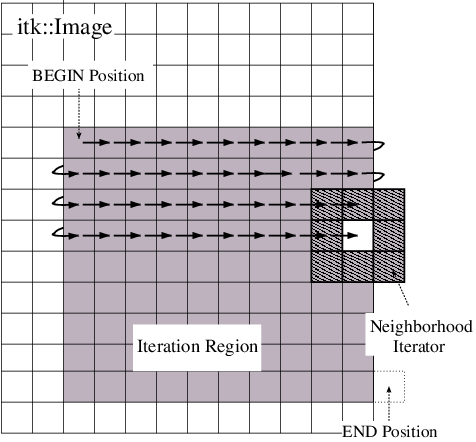
\includegraphics[width=0.6\textwidth]{NeighborhoodIteratorFig1.eps}
\itkcaption[Neighborhood iterator]{Path of a $3x3$ neighborhood
iterator through a 2D image region.  The extent of the neighborhood is
indicated by the hashing around the iterator position. Pixels that lie within
this extent are accessible through the iterator.  An arrow denotes a single
iterator step, the result of one \code{++} operation.}
\protect\label{fig:NeighborhoodIteratorFig1}
\end{figure}

\index{Neighborhood iterators!construction of}
\index{Neighborhood iterators!radius of}

In addition to the standard image pointer and iteration region
(Section~\ref{sec:IteratorsInterface}), neighborhood iterator constructors
require an argument that specifies the extent of the neighborhood to cover.
Neighborhood extent is symmetric across its center in each
axis and is given as an array of $N$ distances that are collectively called the
\emph{radius}. Each element $d$ of the radius, where $0 < d < N$ and
$N$ is the dimensionality of the neighborhood, gives the extent of the
neighborhood in pixels for dimension $N$.  The length of each face of the
resulting ND hypercube is $2d + 1$ pixels, a distance of $d$ on either side of
the single pixel at the neighbor center.
Figure~{\ref{fig:NeighborhoodIteratorFig2} shows the relationship between the
radius of the iterator and the size of the neighborhood for a variety of 2D
iterator shapes.

The radius of the neighborhood iterator is queried after construction
by calling the \code{GetRadius()} method.  Some other methods provide
some useful information about the iterator and its underlying image.

\begin{figure}
\centering
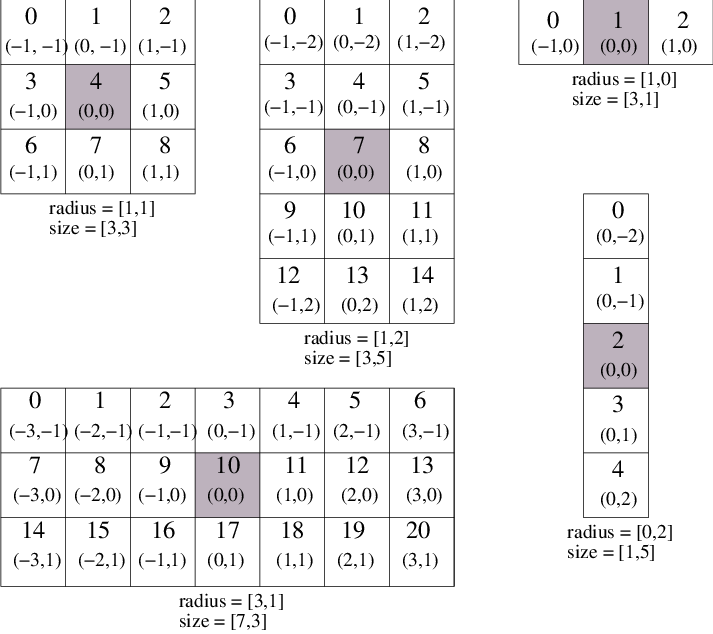
\includegraphics[width=0.9\textwidth]{NeighborhoodIteratorFig2.eps}
\itkcaption[Some possible neighborhood iterator shapes]{Several possible 2D
neighborhood iterator shapes are shown along with their radii and sizes.  A
neighborhood pixel can be dereferenced by its integer index (top) or its
offset from the center (bottom).  The center pixel of each iterator is
shaded.}
\protect\label{fig:NeighborhoodIteratorFig2}
\end{figure}

\begin{itemize}

\index{NeighborhoodIterator!GetRadius()}
\item \textbf{\code{SizeType GetRadius()}} Returns the ND radius of the
neighborhood as an \doxygen{itk}{Size}.

\index{NeighborhoodIterator!GetImagePointer()}
\item \textbf{\code{const ImageType *GetImagePointer()}} Returns the pointer to
the image referenced by the iterator.

\index{NeighborhoodIterator!Size()}
\item \textbf{\code{unsigned long Size()}} Returns the size in number of 
pixels of the neighborhood.

\end{itemize}

The neighborhood iterator interface extends the normal ITK iterator interface
for setting and getting pixel values.  One way to dereference pixels is to
think of the neighborhood as a linear array where each pixel has a unique
integer index. The index of a pixel in the array is determined by incrementing
from the upper-left-forward corner of the neighborhood along the fastest
increasing image dimension: first column, then row, then slice, and so on.  In
Figure~\ref{fig:NeighborhoodIteratorFig2}, the unique integer index is shown
at the top of each pixel.  The center pixel is always at position $n/2$, where
$n$ is the size of the array.

\begin{itemize}

\index{NeighborhoodIterator!GetPixel()}
\item \textbf{\code{PixelType GetPixel(const unsigned int i)}} Returns the 
value of the pixel at neighborhood position \code{i}.

\index{NeighborhoodIterator!SetPixel()}
\item \textbf{\code{void SetPixel(const unsigned int i, PixelType p)}} 
Sets the value of the pixel at position \code{i} to \code{p}.

\end{itemize}

Another way to think about a pixel location in a neighborhood is as an
ND offset from the neighborhood center.  The upper-left-forward corner
of a $3x3x3$ neighborhood, for example, can be described by offset
$(-1, -1, -1)$.  The bottom-right-back corner of the same neighborhood
is at offset $(1, 1, 1)$.  In
Figure~\ref{fig:NeighborhoodIteratorFig2}, the offset from center is
shown at the bottom of each neighborhood pixel.

\begin{itemize}

\index{NeighborhoodIterator!GetPixel()}
\item \textbf{\code{PixelType GetPixel(const OffsetType \&o)}} Get the value of
the pixel at the position offset \code{o} from the neighborhood center.

\index{NeighborhoodIterator!SetPixel()}
\item \textbf{\code{void SetPixel(const OffsetType \&o, PixelType p)}} Set
the value at the position offset \code{o} from the neighborhood center to
the value \code{p}.

\end{itemize}

The neighborhood iterators also provide a shorthand for setting and getting the
value at the center of the neighborhood.

\index{NeighborhoodIterators!}
\begin{itemize}

\index{NeighborhoodIterator!GetCenterPixel()}
\item \textbf{\code{PixelType GetCenterPixel()}} Gets the value at the center
of the neighborhood.

\index{NeighborhoodIterator!SetCenterPixel()}
\item \textbf{\code{void SetCenterPixel(PixelType p)}} Sets the value at the
center of the neighborhood to the value \code{p}

\end{itemize}

There is another shorthand for setting and getting values for pixels that
lie some integer distance from the neighborhood center along one of the image
axes.

\index{NeighborhoodIterators!}
\begin{itemize}

\index{NeighborhoodIterator!GetNext()}
\item \textbf{\code{PixelType GetNext(unsigned int d)}} Get the value
immediately adjacent to the neighborhood center in the positive direction along
the \code{d} axis.

\index{NeighborhoodIterator!SetNext()}
\item \textbf{\code{void SetNext(unsigned int d, PixelType p)}} Set the value
immediately adjacent to the neighborhood center in the positive direction along
the \code{d} axis to the value \code{p}.

\index{NeighborhoodIterator!GetPrevious()}
\item \textbf{\code{PixelType GetPrevious(unsigned int d)}} Get the value
immediately adjacent to the neighborhood center in the negative direction along
the \code{d} axis.

\index{NeighborhoodIterator!SetPrevious()}
\item \textbf{\code{void SetPrevious(unsigned int d, PixelType p)}}
Set the value immediately adjacent to the neighborhood center in the
negative direction along the \code{d} axis to the value \code{p}.

\item \textbf{\code{PixelType GetNext(unsigned int d, unsigned int
s)}} Get the value of the pixel located \code{s} pixels from the
neighborhood center in the positive direction along the \code{d} axis.

\item \textbf{\code{void SetNext(unsigned int d, unsigned int s, PixelType p)}}
Set the value of the pixel located \code{s} pixels from the neighborhood center
in the positive direction along the \code{d} axis to value \code{p}.

\item \textbf{\code{PixelType GetPrevious(unsigned int d, unsigned int
s)}} Get the value of the pixel located \code{s} pixels from the
neighborhood center in the positive direction along the \code{d} axis.
 
\item \textbf{\code{void SetPrevious(unsigned int d, unsigned int s,
PixelType p)}} Set the value of the pixel located \code{s} pixels from
the neighborhood center in the positive direction along the \code{d}
axis to value \code{p}.

\end{itemize}

It is also possible to extract or set all of the neighborhood values
from an iterator at once using a regular ITK neighborhood object.
This may be useful in algorithms that perform a particularly large
number of calculations in the neighborhood and would otherwise require
multiple dereferences of the same pixels.

\begin{itemize}

\index{NeighborhoodIterator!GetNeighborhood()}
\index{NeighborhoodIterator!SetNeighborhood()}
\item \textbf{\code{NeighborhoodType GetNeighborhood()}} Return a
\doxygen{itk}{Neighborhood} of the same size and shape as the neighborhood
iterator and contains all of the values at the iterator position.

\item \textbf{\code{void SetNeighborhood(NeighborhoodType \&N)}} Set all
of the values in the neighborhood at the iterator position to those contained
in Neighborhood \code{N}, which must be the same size and shape as the
iterator.

\end{itemize}

Several methods are defined to provide information about the neighborhood.

\index{NeighborhoodIterators!}
\begin{itemize}

\index{NeighborhoodIterator!GetIndex()}
\item \textbf{\code{IndexType GetIndex()}} Return the image
index of the center pixel of the neighborhood iterator.

\item \textbf{\code{IndexType GetIndex(OffsetType o)}} Return the
image index of the pixel at offset \code{o} from the neighborhood 
center.

\item \textbf{\code{IndexType GetIndex(unsigned int i)}} Return the
image index of the pixel at array position \code{i}.

\index{NeighborhoodIterator!GetOffset()}
\item \textbf{\code{OffsetType GetOffset(unsigned int i)}}  Return the offset
from the neighborhood center of the pixel at array position \code{i}.

\index{NeighborhoodIterator!GetNeighborhoodIndex()}
\item \textbf{\code{unsigned long GetNeighborhoodIndex(OffsetType o)}}
Return the array position of the pixel at offset \code{o} from the
neighborhood center.

\index{NeighborhoodIterator!GetSlice()}
\item \textbf{\code{std::slice GetSlice(unsigned int n)}} Return a
\code{std::slice} through the iterator neighborhood along axis \code{n}.

\end{itemize}

\index{Neighborhood iterators!boundary conditions}
\index{Neighborhood iterators!bounds checking}
A neighborhood-based calculation in a neighborhood close to an image
boundary may require data that falls outside the boundary.  The
iterator in Figure~\ref{fig:NeighborhoodIteratorFig1}, for example, is
centered on a boundary pixel such that three of its neighbors actually
do not exist in the image.  When the extent of a neighborhood falls
outside the image, pixel values for missing neighbors are supplied
according to a rule, usually chosen to satisfy the numerical
requirements of the algorithm.  A rule for supplying out-of-bounds
values is called a \emph{boundary condition}.
 
ITK neighborhood iterators automatically detect out-of-bounds dereferences and
will return values according to boundary conditions.  The boundary condition
type is specified by the second, optional template parameter of the iterator.
By default, neighborhood iterators use a Neumann condition where the first
derivative across the boundary is zero.  The Neumann rule simply returns the
closest in-bounds pixel value to the requested out-of-bounds location.  Several
other common boundary conditions can be found in the ITK toolkit.  They include
a periodic condition that returns the pixel value from the opposite side of the
data set, and is useful when working with periodic data such as Fourier
transforms, and a constant value condition that returns a set value $v$ for all
out-of-bounds pixel dereferences.  The constant value condition is equivalent
to padding the image with value $v$.

Bounds checking is a computationally expensive operation because it occurs each
time the iterator is incremented.  To increase efficiency, a neighborhood
iterator automatically disables bounds checking when it detects that it is
not necessary.  A user may also explicitly disable or enable bounds checking.
Most neighborhood based algorithms can minimize the need for bounds checking
through clever definition of iteration regions.  These techniques are explored
in Section~\ref{sec:NeighborhoodExample3}.

\begin{itemize}

\index{NeighborhoodIterator!NeedToUseBoundaryConditionOn()}
\item \textbf{\code{void NeedToUseBoundaryConditionOn()}} Explicitly turn
bounds checking on.  This method should be used with caution because
unnecessarily enabling bounds checking may result in a significant performance
decrease. In general you should allow the iterator to automatically determine
this setting.

\index{NeighborhoodIterator!NeedToUseBoundaryConditionOff()}
\item \textbf{\code{void NeedToUseBoundaryConditionOff()}} Explicitly disable
bounds checking. This method should be used with caution because disabling
bounds checking when it is needed will result in out-of-bounds reads and
undefined results.

\index{NeighborhoodIterator!OverrideBoundaryCondition()}
\item \textbf{\code{void OverrideBoundaryCondition(BoundaryConditionType *b)}} 
Overrides the templated boundary condition, using boundary condition
object \code{b} instead. Object \code{b} should not be deleted until
it has been released by the iterator.  This method can be used to
change iterator behavior at run-time.

\index{NeighborhoodIterator!ResetBoundaryCondition()}
\item \textbf{\code{void ResetBoundaryCondition()}} Discontinues the use of any
run-time specified boundary condition and returns to using the condition
specified in the template argument.

\index{NeighborhoodIterator!SetPixel()}
\item \textbf{\code{void SetPixel(unsigned int i, PixelType p, bool
status)}} Sets the value at neighborhood array position \code{i} to value
\code{p}.  If the position \code{i} is out-of-bounds, \code{status} is set to
\code{false}, otherwise \code{status} is set to \code{true}.
\end{itemize}

The following sections describe the two ITK neighborhood iterator classes,
\doxygen{itk}{NeighborhoodIterator} and \doxygen{itk}{ShapedNeighborhoodIterator}.
Each has a const and a non-const version.  The shaped iterator is a refinement
of the standard NeighborhoodIterator that supports an
arbitrarily-shaped (non-rectilinear) neighborhood.

\subsection{NeighborhoodIterator}
\label{sec:itkNeighborhoodIterator}

\index{NeighborhoodIterator!examples}
\index{Neighborhood iterators!examples}
The standard neighborhood iterator class in ITK is the
\doxygen{itk}{NeighborhoodIterator}.  Together with its \code{const} version,
\doxygen{itk}{ConstNeighborhoodIterator}, it implements the complete API
described above.  This section provides several examples to illustrate the use
of NeighborhoodIterator.

\index{edge detection}
\index{Sobel operator}
\subsubsection{Basic neighborhood techniques: edge detection}
\label{sec:NeighborhoodExample1}
\input{NeighborhoodIterators1.tex}

\index{convolution filtering}
\index{Sobel operator}
\subsubsection{Convolution filtering: Sobel operator}
\label{sec:NeighborhoodExample2}
\input{NeighborhoodIterators2.tex}

\subsubsection{Optimizing iteration speed}
\label{sec:NeighborhoodExample3}
\input{NeighborhoodIterators3.tex}

\index{Gaussian blurring}
\subsubsection{Separable convolution: Gaussian filtering}
\label{sec:NeighborhoodExample4}
\input{NeighborhoodIterators4.tex}

%% \subsubsection{Slicing the neighborhood}
%% \label{sec:NeighborhoodExample5}
%% \input{NeighborhoodIterators5.tex}

\subsubsection{Random access iteration}
\label{sec:NeighborhoodExample6}
\input{NeighborhoodIterators6.tex}

%./Common/itkConstNeighborhoodIterator.h
%./Common/itkNeighborhoodIterator.h

% Example1: Edge detection using ``hand-coded'' Sobel operator
% Example2: Sobel edge detection using convolution filtering and Sobel operator
% Example3: Improving boundary condition efficiency
% Example4: gaussian filtering, separable convolution
% Example5: Slicing the neighborhood: gaussian filtering, separable convolution
% Example6: Advanced Neighborhood Techniques: local minima, local maxima

\subsection{ShapedNeighborhoodIterator}
\label{sec:itkShapedNeighborhoodIterator}
\index{ShapedNeighborhoodIterator}
\index{Neighborhood iterators!shaped}
\index{Neighborhood iterators!as stencils}
This section describes a variation on the neighborhood iterator called a
\emph{shaped} neighborhood iterator.  A shaped neighborhood is defined like
a bit mask, or \emph{stencil}, with different offsets in the rectilinear
neighborhood of the normal neighborhood iterator turned off or on to create a
pattern.  Inactive positions (those not in the stencil) are not updated during
iteration and their values cannot be read or written.  The shaped iterator is
implemented in the class \doxygen{itk}{ShapedNeighborhoodIterator}, which is a
subclass of
\doxygen{itk}{NeighborhoodIterator}.  A const version,
\doxygen{itk}{ConstShapedNeighborhoodIterator}, is also available.

\index{Neighborhood iterators!active neighbors}
\index{Neighborhood iterators!inactive neighbors}
Like a regular neighborhood iterator, a shaped neighborhood iterator must be
initialized with an ND radius object, but the radius of the neighborhood of a
shaped iterator only defines the set of \emph{possible} neighbors.  Any number
of possible neighbors can then be activated or deactivated.  The shaped
neighborhood iterator defines an API for activating neighbors.  When a neighbor
location, defined relative to the center of the neighborhood, is activated, it
is placed on the \emph{active list} and is then part of the stencil.  An
iterator can be ``reshaped'' at any time by adding or removing offsets from the
active list.

\begin{itemize}

\index{ShapedNeighborhoodIterator!ActivateOffset()}
\item \textbf{\code{void ActivateOffset(OffsetType \&o)}} Include the offset
\code{o} in the stencil of active neighborhood positions.  Offsets are relative
to the neighborhood center.

\index{ShapedNeighborhoodIterator!DeactivateOffset()}
\item \textbf{\code{void DeactivateOffset(OffsetType \&o)}} Remove the offset
\code{o} from the stencil of active neighborhood positions.  Offsets are
relative to the neighborhood center. 

\index{ShapedNeighborhoodIterator!ClearActiveList()}
\item \textbf{\code{void ClearActiveList()}} Deactivate all positions in the
iterator stencil by clearing the active list.

\index{ShapedNeighborhoodIterator!GetActiveIndexListSize()}
\item \textbf{\code{unsigned int GetActiveIndexListSize()}} Return the number
of pixel locations that are currently active in the shaped iterator stencil.

\end{itemize}

Because the neighborhood is less rigidly defined in the shaped iterator, the
set of pixel access methods is restricted.  Only the \code{GetPixel()} and
\code{SetPixel()} methods are available, and calling these methods on an 
inactive neighborhood offset will return undefined results.

For the common case of traversing all pixel offsets in a neighborhood, the
shaped iterator class provides an iterator through the active offsets in its
stencil.   This \emph{stencil iterator} can be incremented or decremented and
defines \code{Get()} and \code{Set()} for reading and writing the values in the
neighborhood.

\begin{itemize}
\index{ShapedNeighborhoodIterator!Iterator::Begin()}
\item \textbf{\code{ShapedNeighborhoodIterator::Iterator Begin()}} Return a
const or non-const iterator through the shaped iterator stencil that points to
the first valid location in the stencil.

\index{ShapedNeighborhoodIterator!Iterator::End()}
\item \textbf{\code{ShapedNeighborhoodIterator::Iterator End()}} Return a
const or non-const iterator through the shaped iterator stencil that points
\emph{one position past} the last valid location in the stencil.
\end{itemize}

The functionality and interface of the shaped neighborhood iterator is best
described by example.  We will use the ShapedNeighborhoodIterator to
implement some binary image morphology algorithms (see \cite{Gonzalez1993},
\cite{Castleman1996}, et al.).  The examples that follow implement erosion and
dilation.

\index{ShapedNeighborhoodIterator!examples of}
\subsubsection{Shaped neighborhoods: morphological operations}
\label{sec:ShapedNeighborhoodExample}
\input{ShapedNeighborhoodIterators1.tex}
\input{ShapedNeighborhoodIterators2.tex}

%./Common/itkConstShapedNeighborhoodIterator.h
%./Common/itkShapedNeighborhoodIterator.h

\index{Iterators!neighborhood|)}

% ADD A SECTION WITH TIPS, SUGGESTIONS ON USING ITERATORS?  EXTENDING ITERATORS?
% USING ITERATORS FOR MULTITHREADING EXAMPLE?
\index{Iterators!image|)}

\input{ImageAdaptors.tex}
\input{StreamingAndThreading.tex}
\chapter{How To Write A Filter}
\label{chapter:WriteAFilter}

This purpose of this chapter is help developers create their own
filter (process object).  This chapter is divided into four major
parts. An initial definition of terms is followed by an overview of
the filter creation process. Next, data streaming is discussed. The
way data is streamed in ITK must be understood in order to write
correct filters. Finally, a section on multithreading describes what
you must do in order to take advantage of shared memory parallel
processing.

\section{Terminology}
\label{sec:Terminology}

The following is some basic terminology for the discussion that follows.
Chapter \ref{chapter:SystemOverview} provides additional background
information.

\begin{itemize}
        \item The \textbf{data processing pipeline} is a directed graph of
        \textbf{process} and \textbf{data objects}. The pipeline inputs,
        operators on, and outputs data.
        \index{data processing pipeline}
        \index{process object}
        \index{data object}

        \item A \textbf{filter}, or \textbf{process object}, has one or more
        inputs, and one or more outputs.
        \index{filter}

        \item A \textbf{source}, or source process object, initiates the data
        processing pipeline, and has one or more outputs.
        \index{source}

        \item A \textbf{mapper}, or mapper process object, terminates the
        data processing pipeline. The mapper has one or more outputs, and may
        write data to disk, interface with a display system, or interface to
        any other system.
        \index{mapper}

        \item A \textbf{data object} represents and provides access to
        data. In ITK, the data object (ITK class \doxygen{itk}{DataObject}) is 
        typically of type \doxygen{otb}{Image} or \doxygen{itk}{Mesh}.
        \index{data object}

        \item A \textbf{region} (ITK class \doxygen{itk}{Region}) represents a 
        piece, or subset of the entire data set.
        \index{region}

        \item An \textbf{image region} (ITK class \doxygen{itk}{ImageRegion})
        represents a structured portion of data. ImageRegion is implemented
        using the \doxygen{itk}{Index} and \doxygen{itk}{Size} classes
        \index{image region}

        \item A \textbf{mesh region} (ITK class \doxygen{itk}{MeshRegion}) 
        represents an unstructured portion of data.
        \index{mesh region}

        \item The \textbf{LargestPossibleRegion} is the theoretical single,
        largest piece (region) that could represent the entire dataset. The
        LargestPossibleRegion is used in the system as the measure of the
        largest possible data size.
        \index{LargestPossibleRegion}

        \item The \textbf{BufferedRegion} is a contiguous block of memory
        that is less than or equal to in size to the
        LargestPossibleRegion. The buffered region is what has actually been
        allocated by a filter to hold its output.
        \index{BufferedRegion}

        \item The \textbf{RequestedRegion} is the piece of the dataset that a
        filter is required to produce. The RequestedRegion is less than or
        equal in size to the BufferedRegion. The RequestedRegion may differ
        in size from the BufferedRegion due to performance reasons. The
        RequestedRegion may be set by a user, or by an application that needs
        just a portion of the data.
        \index{RequestedRegion}

        \item The \textbf{modified time} (represented by ITK class
        \doxygen{itk}{TimeStamp}) is a monotonically increasing integer value that
        characterizes a point in time when an object was last modified.
        \index{modified time}

        \item \textbf{Downstream} is the direction of dataflow, from sources
        to mappers.
        \index{pipeline!downstream}

        \item \textbf{Upstream} is the opposite of downstream, from mappers
        to sources.
        \index{pipeline!upstream}

        \item The \textbf{pipeline modified time} for a particular data
        object is the maximum modified time of all upstream data objects and
        process objects.
        \index{pipeline!modified time}

        \item The term \textbf{information} refers to metadata that
        characterizes data. For example, index and dimensions are information
        characterizing an image region.
        \index{pipeline!information}
\end{itemize}

\section{Overview of Filter Creation}
\label{sec:OverviewFilterCreation}
\index{filter!overview of creation}

\itkpiccaption[Relationship between DataObjects and ProcessObjects]
{Relationship between DataObject and ProcessObject.
\label{fig:DataPipeLineOneConnection}}
\parpic(7cm,2.5cm)[r]{
\includegraphics[width=6cm]{DataPipelineOneConnection.eps}}


Filters are defined with respect to the type of data they input (if
any), and the type of data they output (if any). The key to writing a
ITK filter is to identify the number and types of input and
output. Having done so, there are often superclasses that simplify
this task via class derivation. For example, most filters in ITK take
a single image as input, and produce a single image on output. The
superclass \doxygen{itk}{ImageToImageFilter} is a convenience class that
provide most of the functionality needed for such a filter.

Some common base classes for new filters include:

\begin{itemize}

  \item \code{ImageToImageFilter}: the most common filter base for
    segmentation algorithms.  Takes an image and produces a new image, by
    default of the same dimensions.  Override
    \code{GenerateOutputInformation} to produce a different size.

  \item \code{UnaryFunctorImageFilter}: used when defining a filter that
  applies a function to an image.

  \item \code{BinaryFunctorImageFilter}: used when defining a filter that
  applies an operation to two images.

  \item \code{ImageFunction}: a functor that can be applied to an image,
  evaluating $f(x) $ at each point in the image.

  \item \code{MeshToMeshFilter}: a filter that transforms meshes, such as
  tessellation, polygon reduction, and so on.

  \item \code{LightObject}: abstract base for filters that don't fit well
  anywhere else in the class hierarchy.  Also useful for ``calculator''
  filters; ie. a sink filter that takes an input and calculates a result
  which is retrieved using a \code{Get()} method.

\end{itemize}

Once the appropriate superclass is identified, the filter writer
implements the class defining the methods required by most all ITK
objects: \code{New()}, \code{PrintSelf()}, and protected constructor,
copy constructor, delete, and operator=, and so on. Also, don't forget
standard typedefs like \code{Self}, \code{Superclass}, \code{Pointer}, and
\code{ConstPointer}. Then the filter writer can focus on the most important
parts of the implementation: defining the API, data members, and other
implementation details of the algorithm. In particular, the filter writer
will have to implement either a \code{GenerateData()} (non-threaded) or
\code{ThreadedGenerateData()} method. (See Section~\ref{sec:MultiThreading}
for an overview of multi-threading in ITK.)

An important note: the GenerateData() method is required to allocate memory
for the output. The ThreadedGenerateData() method is not. In default
implementation (see \doxygen{itk}{ImageSource}, a superclass of
\doxygen{itk}{ImageToImageFilter})
\code{GenerateData()} allocates memory and then invokes
\code{ThreadedGenerateData()}.

One of the most important decisions that the developer must make is whether
the filter can stream data; that is, process just a portion of the input to
produce a portion of the output. Often superclass behavior works well: if the
filter processes the input using single pixel access, then the default
behavior is adequate. If not, then the user may have to a) find a more
specialized superclass to derive from, or b) override one or more methods
that control how the filter operates during pipeline execution. The next
section describes these methods.



\section{Streaming Large Data}
\label{sec:StreamingLargeData}
\index{pipeline!streaming large data}

The data associated with multi-dimensional images is large and becoming larger.
This trend is due to advances in scanning resolution, as well as increases in
computing capability. Any practical segmentation and registration software
system must address this fact in order to be useful in application. ITK
addresses this problem via its data streaming facility.

In ITK, streaming is the process of dividing data into pieces, or regions,
and then processing this data through the data pipeline. Recall that the
pipeline consists of process objects that generate data objects, connected
into a pipeline topology. The input to a process object is a data object
(unless the process initiates the pipeline and then it is a source process
object). These data objects in turn are consumed by other process objects,
and so on, until a directed graph of data flow is constructed. Eventually the
pipeline is terminated by one or more mappers, that may write data to
storage, or interface with a graphics or other system. This is illustrated in 
figures \ref{fig:DataPipeLineOneConnection} and \ref{fig:DataPipeLine}.

A significant benefit of this architecture is that the relatively complex
process of managing pipeline execution is designed into the system. This
means that keeping the pipeline up to date, executing only those portions of
the pipeline that have changed, multithreading execution, managing memory
allocation, and streaming is all built into the architecture. However, these
features do introduce complexity into the system, the bulk of which is seen
by class developers. The purpose of this chapter is to describe the pipeline
execution process in detail, with a focus on data streaming.


\subsection{Overview of Pipeline Execution}
\label{sec:OverviewPipelineExecution}
\index{pipeline!overview of execution}

The pipeline execution process performs several important functions.

\begin{figure}
  \par\centering
  \resizebox{5in}{!}{ 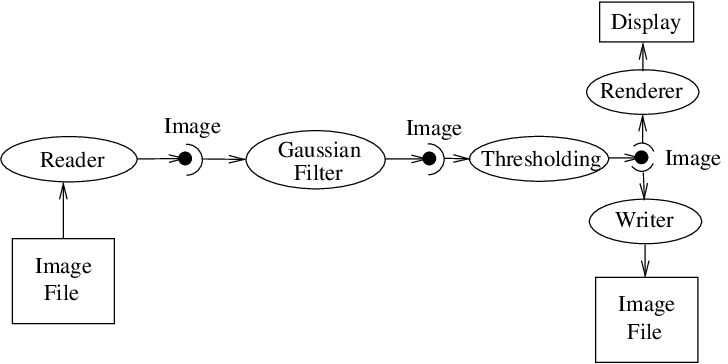
\includegraphics{DataPipeline.eps}} 
  \itkcaption[The Data Pipeline]{The Data Pipeline}
  \label{fig:DataPipeLine}
  \par
\end{figure}

\begin{enumerate}
        \item It determines which filters, in a pipeline of filters, need to
        execute. This prevents redundant execution and minimizes overall
        execution time.

        \item It initializes the (filter's) output data objects, preparing
        them for new data.  In addition, it determines how much memory each
        filter must allocate for its output, and allocates it.

        \item The execution process determines how much data a filter must
        process in order to produce an output of sufficient size for
        downstream filters; it also takes into account any limits on memory
        or special filter requirements. Other factors include the size of
        data processing kernels, that affect how much data input data 
        (extra padding) is required.

        \item It subdivides data into subpieces for multithreading. (Note
        that the division of data into subpieces is exactly same problem as
        dividing data into pieces for streaming; hence multithreading comes
        for free as part of the streaming architecture.)

        \item It may free (or release) output data if filters no longer need
        it to compute, and the user requests that data is to be
        released. (Note: a filter's output data object may be considered a
        ``cache''. If the cache is allowed to remain (\code{ReleaseDataFlagOff()}) 
        between pipeline execution, and the filter, or the input to the 
        filter, never changes, then process objects downstream of the filter 
        just reuse the filter's cache to re-execute.)
\end{enumerate}

To perform these functions, the execution process negotiates with the
filters that define the pipeline. Only each filter can know how much data is
required on input to produce a particular output. For example, a shrink
filter with a shrink factor of two requires an image twice as large (in terms
of its x-y dimensions) on input to produce a particular size output. An
image convolution filter would require extra input (boundary padding)
depending on the size of the convolution kernel. Some filters require the
entire input to produce an output (for example, a histogram), and have the
option of requesting the entire input. (In this case streaming does not work
unless the developer creates a filter that can request multiple pieces,
caching state between each piece to assemble the final output.)


\begin{figure}
  \par\centering
  \resizebox{5in}{!}{ 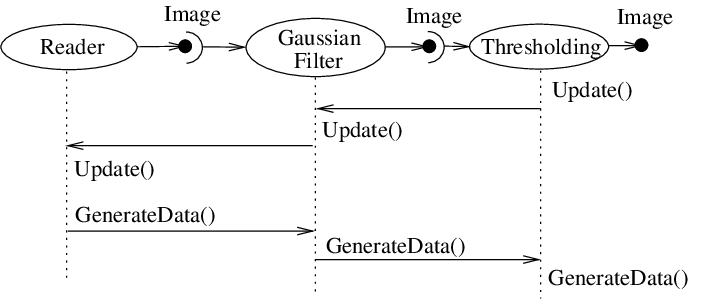
\includegraphics{DataPipelineUpdate.eps}} 
  \itkcaption[Sequence of the Data Pipeline updating mechanism]{Sequence of the
Data Pipeline updating mechanism}
  \label{fig:DataPipeLineUpdate}
  \par
\end{figure}


Ultimately the negotiation process is controlled by the request for data of a
particular size (i.e., region). It may be that the user asks to process a
region of interest within a large image, or that memory limitations result in
processing the data in several pieces. For example, an application may
compute the memory required by a pipeline, and then use
\doxygen{itk}{StreamingImageFilter} to break the data processing into several pieces.
The data request is propagated through the pipeline in the upstream
direction, and the negotiation process configures each filter to produce
output data of a particular size.

The secret to creating a streaming filter is to understand how this
negotiation process works, and how to override its default behavior by using
the appropriate virtual functions defined in \doxygen{itk}{ProcessObject}. The next
section describes the specifics of these methods, and when to override
them. Examples are provided along the way to illustrate concepts.


\subsection{Details of Pipeline Execution}
\label{sec:DetailsPipelineExecution}
\index{pipeline!execution details}

Typically pipeline execution is initiated when a process object
receives the \code{ProcessObject::Update()} method invocation. This
method is simply delegated to the output of the filter, invoking the
\code{DataObject::Update()} method. Note that this behavior is typical
of the interaction between ProcessObject and DataObject: a method
invoked on one is eventually delegated to the other. In this way the
data request from the pipeline is propagated upstream, initiating data
flow that returns downstream.

The \code{DataObject::Update()} method in turn invokes three other methods:

\begin{itemize}
        \item \code{DataObject::UpdateOutputInformation()}
        \item \code{DataObject::PropagateRequestedRegion()}
        \item \code{DataObject::UpdateOutputData()}
\end{itemize}

\subsubsection{UpdateOutputInformation()}
\label{sec:UpdateOutputInformation}
\index{pipeline!UpdateOutputInformation}

The \code{UpdateOutputInformation()} method determines the pipeline modified
time. It may set the RequestedRegion and the LargestPossibleRegion depending
on how the filters are configured. (The RequestedRegion is set to process all
the data, i.e., the LargestPossibleRegion, if it has not been set.) The
UpdateOutputInformation() propagates upstream through the entire pipeline and
terminates at the sources.

During \code{UpdateOutputInformation()}, filters have a chance to override the
\code{ProcessObject::GenerateOutputInformation()} method
(\code{GenerateOutputInformation()} is invoked by
\code{UpdateOutputInformation()}). The default behavior is for the
\code{GenerateOutputInformation()} to copy the metadata describing the input
to the output (via \code{DataObject::CopyInformation()}). Remember, information
is metadata describing the output, such as the origin, spacing,
and LargestPossibleRegion (i.e., largest possible size) of an image.

A good example of this behavior is \doxygen{itk}{ShrinkImageFilter}. This filter
takes an input image and shrinks it by some integral value. The result is that
the spacing and LargestPossibleRegion of the output will be different to that 
of the input. Thus, \code{GenerateOutputInformation()} is overloaded.

\subsubsection{PropagateRequestedRegion()}
\label{sec:PropagateRequestedRegion}
\index{pipeline!PropagateRequestedRegion}

The \code{PropagateRequestedRegion()} call propagates upstream to 
satisfy a data request. In typical application this data request is usually the
LargestPossibleRegion, but if streaming is necessary, or the user is
interested in updating just a portion of the data, the RequestedRegion may be
any valid region within the LargestPossibleRegion.

The function of \code{PropagateRequestedRegion()} is, given a request
for data (the amount is specified by RequestedRegion), propagate
upstream configuring the filter's input and output process object's to
the correct size. Eventually, this means configuring the
BufferedRegion, that is the amount of data actually allocated.

The reason for the buffered region is this: the output of a filter may be
consumed by more than one downstream filter. If these consumers each request
different amounts of input (say due to kernel requirements or other padding
needs), then the upstream, generating filter produces the data to satisfy
both consumers, that may mean it produces more data than one of the
consumers needs.

The \code{ProcessObject::PropagateRequestedRegion()} method invokes
three methods that the filter developer may choose to overload.

\begin{itemize}
        \item \code{EnlargeOutputRequestedRegion(DataObject *output)} gives the
        (filter) subclass a chance to indicate that it will provide more data
        than required for the output. This can happen, for example, when a
        source can only produce the whole output (i.e., the
        LargestPossibleRegion).

        \item \code{GenerateOutputRequestedRegion(DataObject *output)} gives 
        the subclass a chance to define how to set the requested regions for 
        each of its outputs, given this output's requested region.  The default
        implementation is to make all the output requested regions the same.
        A subclass may need to override this method if each output is a
        different resolution. This method is only overridden if a filter has
        multiple outputs.

        \item \code{GenerateInputRequestedRegion()} gives the subclass a 
        chance to
        request a larger requested region on the inputs. This is necessary
        when, for example, a filter requires more data at the ``internal''
        boundaries to produce the boundary values - due to kernel operations
        or other region boundary effects.
\end{itemize}

\doxygen{itk}{RGBGibbsPriorFilter} is an example of a filter that needs to
invoke \code{EnlargeOutputRequestedRegion()}. The designer of this
filter decided that the filter should operate on all the data. Note
that a subtle interplay between this method and
\code{GenerateInputRequestedRegion()} is occurring here. The default
behavior of \code{GenerateInputRequestedRegion()} (at least for
\doxygen{itk}{ImageToImageFilter}) is to set the input RequestedRegion to
the output's ReqestedRegion. Hence, by overriding the method
\code{EnlargeOutputRequestedRegion()} to set the output to the
LargestPossibleRegion, effectively sets the input to this filter to
the LargestPossibleRegion (and probably causing all upstream filters
to process their LargestPossibleRegion as well. This means that the
filter, and therefore the pipeline, does not stream. This could be
fixed by reimplementing the filter with the notion of streaming built
in to the algorithm.)

\doxygen{itk}{GradientMagnitudeImageFilter} is an example of a filter that needs to
invoke \code{GenerateInputRequestedRegion()}. It needs a larger input requested
region because a kernel is required to compute the gradient at a pixel. Hence
the input needs to be ``padded out'' so the filter has enough data to compute
the gradient at each output pixel.

\subsubsection{UpdateOutputData()}
\label{sec:UpdateOutputData}
\index{pipeline!UpdateOutputData}

\code{UpdateOutputData()} is the third and final method as a result of the
\code{Update()} method. The purpose of this method is to determine whether a
particular filter needs to execute in order to bring its output up to date. (A
filter executes when its \code{GenerateData()} method is invoked.) Filter
execution occurs when a) the filter is modified as a result of modifying an
instance variable; b) the input to the filter changes; c) the input data has
been released; or d) an invalid RequestedRegion was set previously and the
filter did not produce data. Filters execute in order in the downstream
direction.  Once a filter executes, all filters downstream of it must also
execute.

\code{DataObject::UpdateOutputData()} is delegated to the DataObject's source
(i.e., the ProcessObject that generated it) only if the DataObject needs to be
updated. A comparison of modified time, pipeline time, release data flag, and
valid requested region is made. If any one of these conditions indicate that
the data needs regeneration, then the source's
\code{ProcessObject::UpdateOutputData()} is invoked. These calls are made
recursively up the pipeline until a source filter object is encountered, or the
pipeline is determined to be up to date and valid. At this point, the recursion
unrolls, and the execution of the filter proceeds. (This means that the output
data is initialized, StartEvent is invoked, the filters \code{GenerateData()}
is called, EndEvent is invoked, and input data to this filter may be released,
if requested. In addition, this filter's InformationTime is updated to the
current time.)

The developer will never override \code{UpdateOutputData()}. The developer need
only write the \code{GenerateData()} method (non-threaded) or
\code{ThreadedGenerateData()} method. A discussion of threading follows in the
next section.


\section{Threaded Filter Execution}
\label{sec:ThreadedFilterExecution}
\index{pipeline!ThreadedFilterExecution}

Filters that can process data in pieces can typically multi-process
using the data parallel, shared memory implementation built into the
pipeline execution process. To create a multithreaded filter, simply
define and implement a \code{ThreadedGenerateData()} method. For
example, a \doxygen{itk}{ImageToImageFilter} would create the method:

\small
\begin{verbatim}
    void ThreadedGenerateData(const OutputImageRegionType& 
                              outputRegionForThread, itk::ThreadIdType threadId)
\end{verbatim}
\normalsize

The key to threading is to generate output for the output region given (as
the first parameter in the argument list above). In ITK, this is simple to do
because an output iterator can be created using the region provided. Hence
the output can be iterated over, accessing the corresponding input pixels as
necessary to compute the value of the output pixel.

Multi-threading requires caution when performing I/O (including using
\code{cout} or \code{cerr}) or invoking events. A safe practice is to allow 
only thread id zero to perform I/O or generate events. (The thread id is
passed as argument into \code{ThreadedGenerateData()}).  If more than one
thread tries to write to the same place at the same time, the program can
behave badly, and possibly even deadlock or crash.


\section{Filter Conventions}
\label{sec:FilterConventions}
\index{pipeline!filter conventions}

In order to fully participate in the ITK pipeline, filters are expected to
follow certain conventions, and provide certain interfaces.  This section
describes the minimum requirements for a filter to integrate into the ITK
framework.

The class declaration for a filter should include the macro
\code{ITK\_EXPORT}, so that on certain platforms an export declaration can be
included. 

A filter should define public types for the class itself (\code{Self}) and
its \code{Superclass}, and \code{const} and non-\code{const} smart pointers,
thus:

\begin{verbatim}
  typedef ExampleImageFilter                Self;
  typedef ImageToImageFilter<TImage,TImage> Superclass;
  typedef SmartPointer<Self>                Pointer;
  typedef SmartPointer<const Self>          ConstPointer;
\end{verbatim}

The \code{Pointer} type is particularly useful, as it is a smart pointer
that will be used by all client code to hold a reference-counted
instantiation of the filter. 

Once the above types have been defined, you can use the following
convenience macros, which permit your filter to participate in the object
factory mechanism, and to be created using the canonical \code{::New()}:

\begin{verbatim}
  /** Method for creation through the object factory. */
  itkNewMacro(Self);  

  /** Run-time type information (and related methods). */
  itkTypeMacro(ExampleImageFilter, ImageToImageFilter);
\end{verbatim}

The default constructor should be \code{protected}, and provide sensible
defaults (usually zero) for all parameters.  The copy constructor and
assignment operator should be declared \code{private} and not implemented,
to prevent instantiating the filter without the factory methods (above). 

Finally, the template implementation code (in the \code{.hxx} file) should
be included, bracketed by a test for manual instantiation, thus:

\begin{verbatim}
#ifndef ITK_MANUAL_INSTANTIATION
#include "itkExampleFilter.hxx"
#endif
\end{verbatim}

\subsection{Optional}
\label{sec:FilterPrinting}
\index{pipeline!printing a filter}

A filter can be printed to an \code{std::ostream} (such as \code{std::cout})
by implementing the following method:

\begin{verbatim}
  void PrintSelf( std::ostream& os, Indent indent ) const;
\end{verbatim}

\noindent and writing the name-value pairs of the filter parameters to the
supplied output stream.  This is particularly useful for debugging.

\subsection{Useful Macros}
\label{sec:UsefulMacros}
\index{pipeline!useful macros}

Many convenience macros are provided by ITK, to simplify filter coding. 
Some of these are described below:

\begin{description}
\item [itkStaticConstMacro] Declares a static variable of the given type,
  with the specified initial value. 
\item [itkGetMacro] Defines an accessor method for the specified scalar data
  member.  The convention is for data members to have a prefix of
  \code{m\_}. 
\item [itkSetMacro] Defines a mutator method for the specified scalar data
  member, of the supplied type.  This will automatically set the
  \code{Modified} flag, so the filter stage will be executed on the next
  \code{Update()}. 
\item [itkBooleanMacro] Defines a pair of \code{OnFlag} and \code{OffFlag}
  methods for a boolean variable \code{m\_Flag}.
\item [itkGetObjectMacro, itkSetObjectMacro] Defines an accessor and mutator
  for an ITK object.  The Get form returns a smart pointer to the object.
\end{description}

Much more useful information can be learned from browsing the source in
\code{Code/Common/itkMacro.h} and for the \doxygen{itk}{Object} and
\doxygen{itk}{LightObject} classes. 



%
% Section on how to write composite filters
%
\input{WriteACompositeFilter.tex}


%
% TODO: include useful tips from mailing list as flagged
%

\input{Persistent.tex}
\chapter{How to write an application}
\label{sec:writeAnApplication}

This chapter presents the different steps to write your own application.
It also contains a description of the framework surrounding the applications.

\section{Application design}
\label{sec:appDesign}
The first logical step is to define the role of your application:
\begin{itemize}
  \item What is the function of your application ? Try to draw a box diagram to 
  describe the design of your application. Note that you don't have to worry 
  about opening and saving image (or vector data) files, this is handled by the 
  framework.
  \item What variables (or data objects) must be exposed outside the application ?
  Try to make a list of the inputs, outputs and parameters of your application.
\end{itemize}
Then you should have a good vision of your application pipeline. Depending on the 
different filters used, the application can be streamed and threaded. The threading
capabilities can be different between the filters so there is no overall threading 
parameter (by default, each filter has its own threading settings). 

It is a different story for streaming. Since the image writers are handled within 
the framework and outside the reach of the developer, the default behaviour is to 
use streaming. If one of the filters doesn't support streaming, it will enlarge 
the requested output region to the largest possible region and the entire image 
will be processed at once. As a result, the developer doesn't have to handle  
streaming nor threading. However, there is a way to choose the number of streaming 
divisions (see section \ref{sec:appParam}).

\section{Architecture of the class}
\label{sec:appArchitecture}
Every application derive from the class \subdoxygen{otb}{Wrapper}{Application}. An 
application can't be templated. It must contain the standard class typedefs and
a call to the \code{OTB\_APPLICATION\_EXPORT} macro.

You need also to define standard macros \doxygen{itk}{NewMacro} and
\doxygen{itk}{TypeMacro}.
 
It is also mandatory to implement three methods in a new application:
\begin{itemize}
  \item \code{DoInit()}
  \item \code{DoUpdateParameters()}
  \item \code{DoExecute()}
\end{itemize}

\subsection{DoInit()}
\label{sec:appDoInit}
This method is called once, when the application is instantiated. It should 
contain the following actions:
\begin{itemize}
  \item Set the name and the description of the application
  \item Fill the documentation and give an example
  \item Declare all the parameters
  \item Define the documentation link:
    \item for contrib application use SetDocLink("\textit{docLink}") function defined in \subdoxygen{otb}{Wrapper}{Application}
    \item for official application use SetOfficialDocLink() function defined in \subdoxygen{otb}{Wrapper}{Application}
\end{itemize}


\subsection{DoUpdateParameters()}
\label{sec:appDoUpdateParameters}
This method is called after every modification of a parameter value. With the command 
line launcher, it is called each time a parameter is loaded. With the Qt launcher, it
is called each time a parameter field is modified. It can be used to maintain consistency and relationship
between parameters (e.g. in ExtractROI: when changing the input image, maybe the ROI size 
has to be updated).

\subsection{DoExecute()}
\label{sec:appDoExecute}
This method contains the real action of the application. This is where the pipeline 
must be set up. The application framework provides different methods to get a value 
or an object associated to a parameter:
\begin{itemize}
  \item \code{GetParameterInt(key)} : get the integer value of a parameter
  \item \code{GetParameterFloat(key)} : get the float value of a parameter
  \item \code{GetParameterString(key)} : get the string value of a parameter
  \item \code{GetParameterImage(key)} : get a pointer to an image object, read from the
  file name given in input
  \item \dots
\end{itemize}

where \code{key} refers to parameter key, defined using \code{AddParameter()} method in \code{DoInit()} method.

Similar methods exist for binding a data object to an output parameter:
\begin{itemize}
  \item \code{SetParameterOutputImage(key,data)} : link the image object to the given output parameter
  \item \code{SetParameterComplexOutputImage(key,data)} : link the complex image object to the given output parameter
  \item \code{SetParameterOutputVectorData(key,data)} : link the vector data object to the given
  output parameter
\end{itemize}

If possible, no filter update should be called inside this function. The update will be 
automatically called afterwards : for every image or vector data output, a writer is 
created and updated.

\subsection{Parameters selection}
\label{sec:appParam}
In the new application framework, every input, output or parameter derive from 
\subdoxygen{otb}{Wrapper}{Parameter}. The application engine supplies the following 
types of parameters:
\begin{itemize}
  \item \code{ParameterType\_Bool} : parameter storing a boolean. 
  \item \code{ParameterType\_Int} : parameter storing an integer.
  \item \code{ParameterType\_Radius} : parameter storing a radius.
  \item \code{ParameterType\_Float} : parameter storing a float.
  \item \code{ParameterType\_String} : parameter storing character string.
  \item \code{ParameterType\_StringList} : parameter storing a list of character string.
  \item \code{ParameterType\_InputFilename} : parameter storing an input file name.
  \item \code{ParameterType\_InputFilenameList} : parameter storing a list of input file names.
  \item \code{ParameterType\_Directory} : parameter storing a folder name.
  \item \code{ParameterType\_Group} : parameter storing children parameters.
  \item \code{ParameterType\_Choice} : parameter storing a list of choices (doesn't support
  multi-choice). It also allows to create specific sub-parameters for each available choice.
  \item \code{ParameterType\_ListView} : parameter storing a list of choices (support 
  multi-choice and single-choice).
  \item \code{ParameterType\_InputImage} : parameter storing an input image.
  \item \code{ParameterType\_InputImageList} : parameter storing a list of input image.
  \item \code{ParameterType\_ComplexInputImage} : parameter storing a complex input image.
  \item \code{ParameterType\_InputVectorData} : parameter storing input vector data.
  \item \code{ParameterType\_InputVectorDataList} : parameter storing a list of input vector data.
  \item \code{ParameterType\_InputProcessXML} : parameter storing an input XML file name.
  \item \code{ParameterType\_OutputFilename} : parameter storing an output file name.
  \item \code{ParameterType\_OutputImage} : parameter storing an output image.
  \item \code{ParameterType\_ComplexOutputImage} : parameter storing a complex output image.
  \item \code{ParameterType\_OutputVectorData} : parameter storing an output vector data.
  \item \code{ParameterType\_OutputProcessXML} : parameter storing an output XML file name.
  \item \code{ParameterType\_RAM} : parameter storing the maximum amount of RAM to be used.
\end{itemize}
\textbf{Note :} The former \code{ParameterType\_Empty} is \textbf{deprecated} and shall be replaced by \code{ParameterType\_Bool}.

\subsection{Parameters description}

Each created parameter has a unique key and several boolean flags to represent its state. These flags
can be used to set a parameter optional or test if the user has modified the parameter value. The parameters
are created in the \code{DoInit()} method, then the framework will set their value (either by parsing the 
command line or reading the graphical user interface). The \code{DoExecute()} method is called when all 
mandatory parameters have been given a value, which can be obtained with "Get" methods defined in 
\subdoxygen{otb}{Wrapper}{Application}. Parameters are set mandatory (or not) using \code{MandatoryOn(key)} method (\code{MandatoryOff(key)}).

Some functions are specific to numeric parameters, such as \code{SetMinimumParameterIntValue(key,value)}
or \code{SetMaximumParameterFloatValue(key,value)}. By default, numeric parameters are treated as inputs.
If your application outputs a number, you can use a numeric parameter and change its role by calling 
\code{SetParameterRole(key,Role\_Output)}.

The input types \code{InputImage}, \code{InputImageList}, \code{ComplexInputImage}, \code{InputVectorData}
and \code{InputVectorDataList} store the name of the files to load, but they also encapsulate the 
readers needed to produce the input data.

The output types \code{OutputImage}, \code{ComplexOutputImage} and \code{OutputVectorData} store the 
name of the files to write, but they also encapsulate the corresponding writers.

\section{Composite application}

The application framework has been extended to allow the implementation of composite applications :
\textbf{applications that use other applications}. The concept is simple : you have two applications A and B
that you want to chain in order to build a third application C. Rather than writing C by copying
the code of A and B, you would like to re-use applications A and B. This plain example will be
re-used in this section for explanations.

A dedicated class \subdoxygen{otb}{Wrapper}{CompositeApplication} has been added to create such applications.
If you derive this class to implement application C, you will be able to create a composite application.

\subsection{Creating internal applications}

Like with standard applications, you have to write a \code{DoInit()} function. In this function,
you should first clean any internal application with the function \code{ClearApplications()}
(the \code{DoInit()} function is called twice in some cases). Then you can
instantiate the internal applications that you want to use (for instance A and B).
The function \code{AddApplication()} will do that, based on :
\begin{itemize}
\item The application type (i.e. its official name, such as ExtractROI, BandMath, \dots)
\item An identifier : like with parameter keys, you have to specify an identifier
to refer to this internal application. Use the same naming conventions as parameters.
\item A description : give a small description of the role of this internal application.
\end{itemize}

Using the function \code{GetInternalApplication()}, you can get a pointer to the
internal application corresponding to a given identifier.

In the example given in introduction, we assume that :
\begin{itemize}
\item An internal application of type A has been added with identifier \code{a}
\item An internal application of type B has been added with identifier \code{b}
\end{itemize}

\subsection{Connecting parameters}

Once you have internal applications, you may want to setup their parameters. There
are typically 3 cases.

You may want to expose a parameter of an internal application as a parameter of
your composite application. Let say you want to expose parameter \code{io.in} from application
\code{a} into your composite application C with the key \code{input}. You can call the function :

\code{ShareParameter("input","a.io.in")}

As a result, the parameters \code{input} in application C and \code{io.in} in application \code{a}
will point to the same object. Under the two parameter keys, there is a unique value.
These two parameters can be considered as synchronized.

This leads to the second case : you may want to synchronize two parameters from internal
applications. Let say you want to synchronize parameter \code{field} from application
\code{a} with parameter \code{fname} from application \code{b}. You can call the function :

\code{Connect("a.field","b.fname")}

Note that the functions \code{ShareParameter()} and \code{Connect()} :
\begin{itemize}
\item Use the same syntax to access internal parameters ("application identifier"
dot "parameter key").
\item Shall be used in the DoInit() function, after the internal applications
have been added.
\end{itemize}

In this synchronization, the two parameters should have the same type, or have a
similar interface, such as input and output filenames that are both accessed using
\code{GetParameterString()} and \code{SetParameterString()}.

This type of connection is a transition to the third case : you may want to connect
the output of an internal application to the input of an other internal application.
Here the difficulty is that the two parameters to connect probably have different
types. Let say you want to connect parameter \code{a.out} to parameter \code{b.in}.
The "Connect()" function may work in favorable cases (see previous paragraph),
but for images, you have two options :
\begin{itemize}
\item Explicitly copy the image pointer from the output image parameter in the input
image parameter (with functions \code{SetParameterInputImage()} and
\code{GetParameterOutputImage()}). It will connect the pipelines in applications
A and B, to form an "in-memory" connexion. This has to be done between the calls
to \code{DoExecute()} of application A and B.
\item Use a temporary filename to store the output image \code{a.out} and read it
with \code{b.in}. In this case, you have to manually call the writers of parameter
\code{a.out}.
\end{itemize}

At the moment, the in-memory connexion of vector data parameters is not supported.

\subsection{Orchestration}

In the \code{DoExecute()} of your composite application, you have to call \code{ExecuteInternal()}
in order to launch each internal application. The order should be compatible with
image parameter connexions. If you want to do "in-memory" connexions, you can do it between
two calls to \code{ExecuteInternal()}, for instance :

\begin{cppcode}
ExecuteInternal("a");
GetInternalApplication("b")->SetParameterInputImage("in",
  GetInternalApplication("a")->GetParameterOutputImage("out"));
ExecuteInternal("b");
\end{cppcode}

The application BundleToPerfectSensor is a simple example of composite applications.
For a more complex example, you can check the application TrainImagesClassifier.

\section{Compile your application}

In order to compile your application you must call the macro \code{OTB\_CREATE\_APPLICATION} in the \emph{CMakelists.txt} file. 
This macro generates the lib \emph{otbapp\_XXX.so}, in (OTB\_BINARY\_DIR/lib/otb/applications), where \emph{XXX} refers to the class name.

\section{Execute your application}

There are different ways to launch applicatons :

\begin{description}
\item[CommandLine :] The command line option is invoked using \emph{otbApplicationLauncherCommandLine} executable followed by the classname, the application dir and the application parameters.
\item[QT :] Application can be encapsuled in Qt framework using \emph{otbApplicationLauncherQt} executable followed by the classname and the application dir.
\item[Python :] A Python wrapper is also available.
\end{description}


\section{Testing your application}
\label{sec:appTesting}
It is possible to write application tests. They are quite similar to filters tests.
The macro \code{OTB\_TEST\_APPLICATION} makes it easy to define a new test.


\section{Application Example}
\label{sec:ApplicationExample}
\ifitkFullVersion
\input{ApplicationExample.tex}
\fi


\chapter{Adding New Modules}
\label{chapter:newModules}

This chapter is concerned with the creation of new modules.
The following sections give precise instructions about :
\begin{itemize}
	\item the organization of your directories
	\item the files you need to include
	\item what they must contain
	\item ...
\end{itemize}

\section{How to Write a Module}
\label{sec:writemodule}

There is a template of OTB remote module which help you  start developing you're
remote module: \href{https://gitlab.orfeo-toolbox.org/remote_modules/remote-module-template}{External Module Template}

Each module is made of different components, which are described in the following sections.

\section{The otb-module.cmake file}

This file is mandatory. It follows the CMake syntax, and has two purposes:

\begin{itemize}
       \item Declare dependencies to other modules,
       \item Provide a short description of the module purpose.
\end{itemize}

These purposes are fulfilled by a single CMake Macro call:

\begin{verbatim}
otb_module(TheModuleName DEPENDS OTBModule1 OTBModule2 ... OTBModuleN DESCRIPTION "A description string")
\end{verbatim}

\textbf{Note}: You can use the keyword TEST\textunderscore DEPENDS to declare module dependencies that only applies to the tests.

\section{The CMakeLists.txt file}

The CMakeLists.txt file is mandatory. It contains only a few things.
First, it declares a new CMake project with the name of the module.

\begin{verbatim}
project(TheModuleName)
\end{verbatim}

Second, if the module contain a library (see src folder section below), it initializes the TheModuleName\textunderscore LIBRARIES CMake variable (if your module only contains headers or template code, skip this line):

\begin{verbatim}
set(TheModuleName_LIBRARIES OTBTheModuleName)
\end{verbatim}

You can build your remote modules inside the OTB source tree by copying your
source inside the directory \textit{Module/Remote} or against an existing OTB
build tree (note that it does not work with an install version of OTB).

The configuration below will handle both cases and take care of all the CMake
plumbing of the module:

\begin{verbatim}
  if(NOT OTB_SOURCE_DIR)
    find_package(OTB REQUIRED)
    list(APPEND CMAKE_MODULE_PATH ${OTB_CMAKE_DIR})
    include(OTBModuleExternal)
  else()
    otb_module_impl()
  endif()
\end{verbatim}

The overall file should look like this:

\begin{verbatim}
cmake_minimum_required(VERSION 2.8.9)
project(TheModuleName)
set(ExternalTemplate_LIBRARIES OTBTheModuleName)

if(NOT OTB_SOURCE_DIR)
    find_package(OTB REQUIRED)
    list(APPEND CMAKE_MODULE_PATH ${OTB_CMAKE_DIR})
    include(OTBModuleExternal)
  else()
    otb_module_impl()
  endif()
\end{verbatim}

\section{The include folder}

The include folder will contain all your headers (*.h files) and template method boy files (*.hxx or *.hxx). It does not require any additional file (in particular, no CMakeLists.txt file is required).

\section{The src folder }

The src folder contains the internal implementation of your module :

\begin{itemize}
       \item  It typically contains cxx source files that will be compiled into a library.
       \item  It can contain header files for classes used only within the implementation files of your module. Any header file present in the src folder will not be installed, and will not be available to other modules depending on your module.
\end{itemize}

If your modules is made of template only code, you do not need a src folder at all.

If present, the src folder requires a CMakeLists.txt file.

The first part of the CMakeLists.txt file is classical, as it builds the library and links it:

\begin{verbatim}
set(OTBTheModuleName_SRC
    sourceFile1.cxx
    sourceFile2.cxx
    sourceFile3.cxx
    ...
    sourceFileN.cxx)

add_library(OTBTheModuleName ${OTBTheModuleName_SRC})

target_link_libraries(OTBTheModuleName ${OTBModule1_LIBRARIES} ${OTBModule2_LIBRARIES} ... ${OTBModuleN_LIBRARIES})
\end{verbatim}

\textbf{Notes}:

\begin{itemize}
       \item  Library name should match the one declared in the root CMakeLists.txt when setting CMake variable TheModuleName\textunderscore LIBRARIES,
       \item  Linked libraries should match the dependencies of your module declared in the root otb-module.cmake file.
\end{itemize}

The last line of CMake code takes care of installation instructions:
\begin{verbatim}
otb_module_target(TBTheModuleName)
\end{verbatim}

The overall CMakeLists.txt file should look like:

\begin{verbatim}
set(OTBTheModuleName_SRC
    sourceFile1.cxx
    sourceFile2.cxx
    sourceFile3.cxx
    ...
    sourceFileN.cxx)

add_library(OTBTheModuleName ${OTBTheModuleName_SRC})

target_link_libraries(OTBTheModuleName ${OTBModule1_LIBRARIES} ${OTBModule2_LIBRARIES} ... ${OTBModuleN_LIBRARIES})

otb_module_target(TBTheModuleName)
\end{verbatim}

\section{The app folder}

The app folder contains the code of applications shipped with your module. If your module has no application, you do not need the app folder.

\textbf{Notes}: If your module contains application (and an app folder), do not forget to add the ApplicationEngine in the dependencies listed in the otb-module.cmake file.

In addition to the applications source code, the app folder should contain a CMakeLists.txt file as follows.

For each application, a single call otb\textunderscore create\textunderscore application is required:

\begin{verbatim}
otb_create_application(
 NAME           TheModuleApplication1
 SOURCES        TheModuleApplication1.cxx
 LINK_LIBRARIES ${OTBModule1_LIBRARIES} ${OTBModule2_LIBRARIES} ... ${OTBModuleN_LIBRARIES})

\end{verbatim}

\section{The test folder}

This folder contains tests of the module. If your module has no test in it (which is not recommended, you do not need it).

The test folder should contain the source files of tests, as well as a CMakeLists.txt file. This file will contain the following.

First, indicate that this folder contains tests.

\begin{verbatim}
otb_module_test()
\end{verbatim}

Then, build the test driver:

\begin{verbatim}
set(OTBTheModuleNameTests
    testFile1.cxx
    testFile2.cxx
    ...
    testFileN.cxx)

add_executable(otbTheModuleNameTestDriver ${OTBTheModuleNameTests})

target_link_libraries(otbTheModuleNameTestDriver ${OTBTheModuleName-Test_LIBRARIES})

otb_module_target_label(otbTheModuleNameTestDriver)
\end{verbatim}

Finally, you can add your tests:

\begin{verbatim}
otb_add_test(NAME nameOfTheTest COMMAND otbTheModuleNameTestDriver
             --compare-image ${EPSILON_8} ... # baseline comparison if needed
             nameOfTheTestFunction
             testParameters)
\end{verbatim}

If your module contains one or more application in the app folder, you should
also write tests for them, in the test folder. Running an application test is
easily done with the helper macro otb\textunderscore test\textunderscore
application:

\begin{verbatim}
otb_test_application(NAME   nameofApplication1Test1
                      APP  TheModuleApplication1
                      OPTIONS -in1 ${INPUTDATA}/input1.tif
                              -in2 ${INPUTDATA}/input2.tif
                              -out ${TEMP}/nameofApplication1Test1_result.tif
                      VALID   --compare-image ${EPSILON_8}
                              ${BASELINE}/nameofApplication1Test1_result.tif
                              ${TEMP}/nameofApplication1Test1_result.tif)
\end{verbatim}

ToDo: Add instructions for test naming and input/baseline data inclusion.

You overall CMakeLists.txt file should look like:

\begin{verbatim}
otb_module_test()

set(OTBTheModuleNameTests
    testFile1.cxx
    testFile2.cxx
    ...
    testFileN.cxx)

add_executable(otbTheModuleNameTestDriver ${OTBTheModuleNameTests})

target_link_libraries(otbTheModuleNameTestDriver ${OTBTheModuleName-Test_LIBRARIES})

otb_module_target_label(otbTheModuleNameTestDriver)

otb_add_test(NAME nameOfTheTest COMMAND otbTheModuleNameTestDriver
             --compare-image ${EPSILON_8} ... # baseline comparison if needed
             nameOfTheTestFunction
             testParameters)
\end{verbatim}

\section{Including a remote module in OTB}
\begin{itemize}
       \item Local build of a remote module
\end{itemize}

Your remote module can be build inside the OTB source tree or outside as a
external CMake project with an existing OTB. Please note in that case
that you'll have to set OTB\textunderscore DIR CMake option.

If OTB\textunderscore DIR is an OTB build tree, there are two ways of compiling:
\begin{itemize}
  \item Build as a module, in which case build files will be written
    to the OTB build tree as other modules. Main benefit is that this
    will enrich the current OTB build with your new module, but you
    need to have write access to the build directory.
  \item Build as a standalone CMake project, in which case build files
    will remain in the module build folder. This build is fully
    independent from the build (or install) directory, but the module
    will not be recognized as an OTB module (still you will be able to
    use its binaries and libraries).
\end{itemize}

This behaviour is controlled by the OTB\textunderscore BUILD\textunderscore MODULE\textunderscore AS\textunderscore STANDALONE, which is OFF by default (hence first behaviour).

Note that when dealing with an installed OTB, only the second behaviour (build as standalone) is available.

Optionally, you can build your new remote module inside the OTB source tree by simply copy
the folder containing the module component to Modules/Remote, then run CMake
configuration. you should see a new CMake option named MODULE\textunderscore
TheModuleName. Simply turn this option to ON, and finish CMake
configuration. Your module will be built with the rest of the OTB project.

\begin{itemize}
       \item  Sharing your remote module
\end{itemize}

To make your remote module available to others when building OTB, you should
provide a CMake file named TheModuleName.remote.cmake file for inclusion in the
Modules/Remote folder in OTB source tree.

This file should contain the following:

\begin{verbatim}
#Contact: Author name <author email address>

otb_fetch_module(TheModuleName
  "A description of the module, to appear during CMake configuration step"
  GIT\textunderscore REPOSITORY http\textunderscore link\textunderscore to\textunderscore a\textunderscore git\textunderscore repository\textunderscore hosting\textunderscore the\textunderscore module
  GIT\textunderscore TAG the\textunderscore git\textunderscore revision\textunderscore to\textunderscore checkout
  )
\end{verbatim}
This file should be provided along with your remote module inclusion proposal email to the otb-developers list. Please refer to the contributors guidelines for more information (next section).

\chapter{Contributors Guidelines}
\label{chapter:Contribute}

See
\url{https://gitlab.orfeo-toolbox.org/orfeotoolbox/otb/blob/develop/CONTRIBUTING.md}
in OTB sources.




\part{Appendix}\label{part:appendix}

\input{Contributors.tex}

\backmatter

%%%%%%%%%%%%%%%%%%%%%%%%%%%%%%%%%%%%%%%%%
%
%  Insert the bibliography using BibTeX
%
%%%%%%%%%%%%%%%%%%%%%%%%%%%%%%%%%%%%%%%%%

% \bibliographystyle{plain}
\bibliographystyle{abbrv}
\bibliography{\bibtexdatabasepath/Insight}


%%%%%%%%%%%%%%%%%%%%%%%%%%%%%%%%%%%%%%%%%
%
%  Insert the Index file
%
%%%%%%%%%%%%%%%%%%%%%%%%%%%%%%%%%%%%%%%%%

\InputIfFileExists{SoftwareGuide.ind}{}{}

%%\ifitkPrintedVersion
%%\cleardoublepage
%%% \input{MarketingMaterial.tex}
%%\fi

\end{document}



